%%%%%%%%%%%%%%%%%%%%%%%%%%%%%%%%%%%%%%%%%%%%%%%%%%%
%
%  New template code for TAMU Theses and Dissertations starting Spring 2018.  
%
%
%  Author: Sean Zachary Roberson
%  Version 3.17.09
%  Last Updated: 9/21/2017
%
%%%%%%%%%%%%%%%%%%%%%%%%%%%%%%%%%%%%%%%%%%%%%%%%%%%

% NOTE: THE ONLY MAJOR CHANGE IS IN THE RELAXATION
% OF MARGIN REQUIREMENTS. THIS TEMPLATE IS THE MOST
% CURRENT. SEE THE FILES README.TXT AND NEWCHANGES.TXT
% FOR MORE INFORMATION.

\documentclass[12pt]{report}

\usepackage{tamuconfig}

% Most of the packages that set the default settings
% for the document have moved to the style file
% tamuconfig.sty. This includes

%These next lines change the font. Fixes for certain
%fonts will be implemented in a future release.

%Comment this line if you do not wish to use Times
%New Roman. The font used will then be the LaTeX
%default of Computer Modern.
\usepackage{times}
%\usepackage{cmbright}
\usepackage[T1]{fontenc}

% For natbib-style references, uncomment this.
%\usepackage{natbib}

%This package allows for the use of graphics in the
%document.
\usepackage{graphicx}

%If you have JPEG format images, add .jpg as an
%allowed file extension below. Same for Bitmaps (.bmp).
\DeclareGraphicsExtensions{.png, .pdf, .jpg}

%It is best practice to keep all your pictures in
%one folder inside the main directory in which your
%TeX file is kept. Here the folder is named "graphic."
%Replace the name here with your folder's name, if needed.
%The period is needed due to relative referencing.
\graphicspath{ {./graphic/} }

% For quick document navigation.
\usepackage[hidelinks]{hyperref}

%%%%%%%%%%%%%%%%%%%%%%%%%%%%%%%%%%%%%%%%%%%%%%%%%%%%%%%%%
%Please place all your personal packages here. Check to
%see if the packages you wish to use are not already
%declared above. Placing all your personal packages
%here allows me to determine if there are any package
%issues in compilation, as well as any conflicts
%that may arise by the order of loading.
%--Sean Zachary Roberson
%%%%%%%%%%%%%%%%%%%%%%%%%%%%%%%%%%%%%%%%%%%%%%%%%%%%%%%%%
%%%%%%%%%%%%%%%%%%%%%%%%%%%%%%%%%%%%%%%%%%%%%%%%%%%%%%%%%
%Begin student defined packages.
%%%%%%%%%%%%%%%%%%%%%%%%%%%%%%%%%%%%%%%%%%%%%%%%%%%%%%%%%
%To use sub-figures
\usepackage[font=footnotesize]{caption}
\usepackage{subcaption}
% to enhance tables presentation
\usepackage{multirow}
\usepackage{array}
% To brake long citations to the next line.
\usepackage{cite}
\usepackage{microtype}
\microtypesetup{protrusion=false}

%%%%%%%%%%%%%%%%%%%%%%%%%%%%%%%%%%%%%%%%%%%%%%%%%%%%%%%%%
%End student defined packages.
%%%%%%%%%%%%%%%%%%%%%%%%%%%%%%%%%%%%%%%%%%%%%%%%%%%%%%%%%

% End preamble. Document begins below.

\begin{document}

%The title of your document goes here.
%Spacing may need to be adjusted if your title is long
%and pushes the copyright off the page.
\renewcommand{\tamumanuscripttitle}{Application of the Generalized Finite Element Method to the Acoustic Wave Simulation in Exploration Seismology}

%Type only Thesis, Dissertation, or Record of Study.
\renewcommand{\tamupapertype}{Thesis}

%Your full name goes here, as it is in university records. Check your student record on Howdy if there is any mismatch.
\renewcommand{\tamufullname}{Edith Sotelo Gamboa}

%The degree title goes here. See the OGAPS site for more info.
\renewcommand{\tamudegree}{Master of Science}

\renewcommand{\tamuchairone}{Richard L. Gibson, Jr.}

% Uncomment out the next line if you have co-chairs.  You will also need to edit the titlepage.tex file.
%\newcommand{\tamuchairtwo}{Additional Chair Name}
\renewcommand{\tamumemberone}{Benchun Duan}
\newcommand{\tamumembertwo}{Yalchin R. Efendiev}
%\newcommand{\tamumemberthree}{Dr. Yalchin R. Efendiev}
\renewcommand{\tamudepthead}{Michael Pope}

%Type only May, August, or December.
\renewcommand{\tamugradmonth}{December}
\renewcommand{\tamugradyear}{2018}
%Your department name goes here.
\renewcommand{\tamudepartment}{Geophysics}


%%%%%%%%%%%%%%%%%%%%%%%%%%%%%%%%%%%%%%%%%%%%%%%%%%%
%
%  New template code for TAMU Theses and Dissertations starting Fall 2016.  
%
%
%  Author: Sean Zachary Roberson
%  Version 3.17.09
%  Last Updated: 9/21/2017
%
%%%%%%%%%%%%%%%%%%%%%%%%%%%%%%%%%%%%%%%%%%%%%%%%%%%

%%%%%%%%%%%%%%%%%%%%%%%%%%%%%% 
%% TITLE PAGE
%% The values get updated automatically.  Please do not make changes to this file other than adding/deleting committee members where necessary.
%%%%%%%%%%%%%%%%%%%%%%%%%%%%%%

\providecommand{\tabularnewline}{\\}



\begin{titlepage}
\begin{center}
\MakeUppercase{\tamumanuscripttitle}
\vspace{4em}

A \tamupapertype

by

\MakeUppercase{\tamufullname}

\vspace{4em}

\begin{singlespace}

Submitted to the Office of Graduate and Professional Studies of \\
Texas A\&M University \\

in partial fulfillment of the requirements for the degree of \\
\end{singlespace}

\MakeUppercase{\tamudegree}
\par\end{center}
\vspace{2em}
\begin{singlespace}
\begin{tabular}{ll}
 & \tabularnewline
& \cr
% If you have Co-Chairs comment out the 'Chair of Committee' line below and uncomment the 'Co-Chairs of Committee' line.
Chair of Committee, & \tamuchairone\tabularnewline
%Co-Chairs of Committee, & \tamuchairone\tabularnewline & \tamuchairtwo\tabularnewline
Committee Members, & \tamumemberone\tabularnewline
 & \tamumembertwo\tabularnewline
% & \tamumemberthree\tabularnewline
Head of Department, & \tamudepthead\tabularnewline

\end{tabular}
\end{singlespace}
\vspace{3em}

\begin{center}
\tamugradmonth \hspace{2pt} \tamugradyear

\vspace{3em}

Major Subject: \tamudepartment \par
\vspace{3em}
Copyright \tamugradyear \hspace{.5em}\tamufullname 
\par\end{center}
\end{titlepage}
\pagebreak{}




 % This is simply a file that formats and adds your titlepage, please do not edit this unless you have a specific need. .
%%%%%%%%%%%%%%%%%%%%%%%%%%%%%%%%%%%%%%%%%%%%%%%%%%%
%
%  New template code for TAMU Theses and Dissertations starting Fall 2016.  
%
%
%  Author: Sean Zachary Roberson
%  Version 3.17.09
%  Last Updated: 9/21/2017
%
%%%%%%%%%%%%%%%%%%%%%%%%%%%%%%%%%%%%%%%%%%%%%%%%%%%
%%%%%%%%%%%%%%%%%%%%%%%%%%%%%%%%%%%%%%%%%%%%%%%%%%%%%%%%%%%%%%%%%%%%%
%%                           ABSTRACT 
%%%%%%%%%%%%%%%%%%%%%%%%%%%%%%%%%%%%%%%%%%%%%%%%%%%%%%%%%%%%%%%%%%%%%

\chapter*{ABSTRACT}
\addcontentsline{toc}{chapter}{ABSTRACT} % Needs to be set to part, so the TOC doesnt add 'CHAPTER ' prefix in the TOC.

\pagestyle{plain} % No headers, just page numbers
\pagenumbering{roman} % Roman numerals
\setcounter{page}{2}

\indent Numerical methods for the simulation of wave propagation have extensive applications in exploration seismology as in velocity estimation and subsurface imaging. Among numerical methods, the standard finite element method (FEM) presents important advantages such as the ability to handle meshes to conform to complex geometry, making this technique attractive. However its main drawback is the longer simulation time it may take compared to other numerical techniques. Nonetheless, a modified version, the generalized finite element method (GFEM), has the potential to overcome this limitation. Hence,
I have applied the GFEM to simulate the acoustic wave propagation to test its performance against the standard FEM in models that are relevant to exploration seismology. The GFEM exploits the partition of unity property of the FEM standard basis functions by incorporating additional user-defined enrichment functions to improve the efficiency of the simulation. Specifically, I have incorporated plane waves at different directions to mimic the radial propagation of transient acoustic waves, with the goal of accelerating the solution convergence. I have tested this approach  using models of interest in  exploration seismology, including a low velocity layer, a karst structure and topography. Results from these specific models show that the GFEM approach is more efficient than a standard FEM reference solution, with an acceptable solution accuracy.

\pagebreak{}

%%%%%%%%%%%%%%%%%%%%%%%%%%%%%%%%%%%%%%%%%%%%%%%%%%%
%
%  New template code for TAMU Theses and Dissertations starting Fall 2016.  
%
%
%  Author: Sean Zachary Roberson
%  Version 3.17.09
%  Last Updated: 9/21/2017
%
%%%%%%%%%%%%%%%%%%%%%%%%%%%%%%%%%%%%%%%%%%%%%%%%%%%

%%%%%%%%%%%%%%%%%%%%%%%%%%%%%%%%%%%%%%%%%%%%%%%%%%%%%%%%%%%%%%%%%%%%%%
%%                           DEDICATION
%%%%%%%%%%%%%%%%%%%%%%%%%%%%%%%%%%%%%%%%%%%%%%%%%%%%%%%%%%%%%%%%%%%%%
\chapter*{DEDICATION}
\addcontentsline{toc}{chapter}{DEDICATION}  % Needs to be set to part, so the TOC doesnt add 'CHAPTER ' prefix in the TOC.



\begin{center}
\vspace*{\fill}
To my mother, father and  sisters. Thank you for your unconditional support.
\vspace*{\fill}
\end{center}

\pagebreak{}

%%%%%%%%%%%%%%%%%%%%%%%%%%%%%%%%%%%%%%%%%%%%%%%%%%%
%
%  New template code for TAMU Theses and Dissertations starting Fall 2016.  
%
%
%  Author: Sean Zachary Roberson
%  Version 3.17.09
%  Last Updated: 9/21/2017
%
%%%%%%%%%%%%%%%%%%%%%%%%%%%%%%%%%%%%%%%%%%%%%%%%%%%


%%%%%%%%%%%%%%%%%%%%%%%%%%%%%%%%%%%%%%%%%%%%%%%%%%%%%%%%%%%%%%%%%%%%%%
%%                           ACKNOWLEDGMENTS
%%%%%%%%%%%%%%%%%%%%%%%%%%%%%%%%%%%%%%%%%%%%%%%%%%%%%%%%%%%%%%%%%%%%%
\chapter*{ACKNOWLEDGMENTS}
\addcontentsline{toc}{chapter}{ACKNOWLEDGMENTS}  % Needs to be set to part, so the TOC doesnt add 'CHAPTER ' prefix in the TOC.


\indent I would like to thank my advisor, Dr. Gibson, for his guidance and scientific insight throughout this process. I am also grateful with the Department of Geology and Geophysics for providing financial support through teaching assistanship to complete the degree.

\pagebreak{}
%%%%%%%%%%%%%%%%%%%%%%%%%%%%%%%%%%%%%%%%%%%%%%%%%%%
%
%  New template code for TAMU Theses and Dissertations starting Fall 2016.  
%
%
%  Author: Sean Zachary Roberson
%  Version 3.17.09
%  Last Updated: 9/21/2017
%
%%%%%%%%%%%%%%%%%%%%%%%%%%%%%%%%%%%%%%%%%%%%%%%%%%%


%%%%%%%%%%%%%%%%%%%%%%%%%%%%%%%%%%%%%%%%%%%%%%%%%%%%%%%%%%%%%%%%%%%%%%
%%             CONTRIBUTORS AND FUNDING SOURCES
%%%%%%%%%%%%%%%%%%%%%%%%%%%%%%%%%%%%%%%%%%%%%%%%%%%%%%%%%%%%%%%%%%%%%
\chapter*{CONTRIBUTORS AND FUNDING SOURCES}
\addcontentsline{toc}{chapter}{CONTRIBUTORS AND FUNDING SOURCES}  % Needs to be set to part, so the TOC doesn't add 'CHAPTER ' prefix in the TOC.


%This section is taken directly from the MS Word templates.

%Old version below.

%All theses and dissertations must include a contributors and funding sources section. In this section, name all members of the dissertation committee, and any collaboration with others in carrying out your thesis or dissertation research. Your independent contributions must be made clear.
%
%If financial support from the university or any other source was gained to conduct your thesis or dissertation research and compilation, it must be listed in this section. If you completed all work independently without outside financial support, indicate this here.
%\textit{(Sample Wording)}
%
%This work was supported by a dissertation committee consisting of Professor XXX [advisor – also note if co-advisor] and XXXX of the Department of [Home Department] and Professor(s) XXXX of the Department of [Outside Department].
% 
%The data analyzed for Chapter III was provided by Professor XXXX. The analyses depicted in Chapter IV were conducted in part by Rebecca Jones of the Department of Biostatistics and were published in (year) in an article listed in the Biographical Sketch. 
%
%All other work conducted for the dissertation was completed by the student independently.
%
%\noindent \textit{(or)}
%
%This work was supervised by a dissertation committee consisting of Professor XXXX [advisor – also note if co-advisor] and Professor(s) XXXX of the Department of [Home Department] and Professor(s) XXXX of [Outside Department]. All work for the dissertation was completed independently by the student.
%
%\noindent \textit{(or)}
%
%Graduate study was supported by a fellowship from Texas A\&M University and a dissertation research fellowship from XXX Foundation.

\subsection*{Contributors}
This work was supported by a thesis committee consisting of Professor Richard Gibson and  Professor Benchun Duan of the Department of Geology and Geophysics and Professor Yalchin Efendiev of the Department of Mathematics.

Denis Davydov, deal.II  developer, provided technical support for the implementation of the GFEM code using the deal.II library.

All other work conducted for the thesis was completed by the student independently.
\subsection*{Funding Sources}
Graduate study was supported by a teaching assistantship from the Department of Geology and Geophysics at Texas A\&M University.
\pagebreak{}
%%%%%%%%%%%%%%%%%%%%%%%%%%%%%%%%%%%%%%%%%%%%%%%%%%%%
%
%  New template code for TAMU Theses and Dissertations starting Fall 2016.  
%
%
%  Author: Sean Zachary Roberson
%  Version 3.17.09
%  Last Updated: 9/21/2017
%
%%%%%%%%%%%%%%%%%%%%%%%%%%%%%%%%%%%%%%%%%%%%%%%%%%%

%%%%%%%%%%%%%%%%%%%%%%%%%%%%%%%%%%%%%%%%%%%%%%%%%%%%%%%%%%%%%%%%%%%%%%
%%                           NOMENCLATURE
%%%%%%%%%%%%%%%%%%%%%%%%%%%%%%%%%%%%%%%%%%%%%%%%%%%%%%%%%%%%%%%%%%%%%

\chapter*{NOMENCLATURE}
\addcontentsline{toc}{chapter}{NOMENCLATURE}  % Needs to be set to part, so the TOC doesnt add 'CHAPTER ' prefix in the TOC.

%A note about aligning: These entries will align
%themselves according to the ampersand (&).
%No extra spaces are needed, as seen in some of
%the entries below.

%Example of the longtable environment.
\hspace*{-1.25in}
\vspace{12pt}
\begin{spacing}{1.0}
	\begin{longtable}[htbp]{@{}p{0.35\textwidth} p{0.62\textwidth}@{}}
	   % \begin{tabular}{@{}p{0.33\textwidth} p{0.62\textwidth}@{}}
		OGAPS	&	Office of Graduate and Professional Studies at Texas A\&M University\\	[2ex]
		B/CS		&	Bryan and College Station\\	[2ex] %[2ex] provides double space between each row
		TAMU			&	Texas A\&M University\\	[2ex]
		SDCC & San Diego Comic-Con\\ [2ex]
		EVIL & Every Villain is Lemons\\ [2ex]
		EPCC & Educator Preparation and Certification Center at Texas A\&M University - San Antonio\\ [2ex]
		FFT & Fast Fourier Transform\\ [2ex]
		ARIMA & Autoregressive Integrated Moving Average\\ [2ex]
		SSD & Solid State Drive\\ [2ex]
		HDD & Hard Disk Drive\\ [2ex]
		O\&M & Eller Oceanography and Meteorology Building\\ [2ex]
		DOS & Disk Operating System\\ [2ex]
		HDMI & High Definition Multimedia Interface\\ [2ex]
		$L^1$ & Space of absolutely Lebesgue integrable functions; i.e., $\int |f| < \infty$\\ [2ex]
		$L^2$ & Space of square-Lebesgue-integrable functions, i.e., $\int |f|^2 < \infty$\\ [2ex]
		$PC(S)$ & Space of piecewise-continuous functions on $S$\\ [2ex]
		GNU & GNU is Not Unix\\ [2ex]
		GUI & Graphical User Interface\\ [2ex]
		PID & Principal Integral Domain\\ [2ex]
		MIP & Mixed Integer Program\\ [2ex]
		LP & Linear Program\\ [2ex]
		%XXXXXXXX		&	This is an optional page. Random word to test how long the sentence can be? This is just for test purpose. The current setting aims to align left/right margin same as all other pages.\\	[2ex]
	   % \end{tabular}%
	\end{longtable}
\end{spacing}

\pagebreak{}

%%%%%%%%%%%%%%%%%%%%%%%%%%%%%%%%%%%%%%%%%%%%%%%%%%%
%
%  New template code for TAMU Theses and Dissertations starting Fall 2016.  
%
%
%  Author: Sean Zachary Roberson
%  Version 3.17.09
%  Last Updated: 9/21/2017
%
%%%%%%%%%%%%%%%%%%%%%%%%%%%%%%%%%%%%%%%%%%%%%%%%%%%
%%%%%%%%%%%%%%%%%%%%%%%%%%%%%%%%%%%%%%%%%%%%%%%%%%%%%%%%%%%%%%%%%%%%%%
%%       TABLE OF CONTENTS
%%%%%%%%%%%%%%%%%%%%%%%%%%%%%%%%%%%%%%%%%%%%%%%%%%%%%%%%%%%%%%%%%%%%%
% single-space sections in Table of Contents  - commented in version 1.7
%\renewcommand{\cftsecafterpnum}{\vskip0.5\baselineskip}
%\renewcommand{\cftsubsecafterpnum}{\vskip0.5\baselineskip}
%\renewcommand{\cftsubsubsecafterpnum}{\vskip0.5\baselineskip}
%%%%%%%%%%%%%%%%%%%%%%%%%%%%%%%%%%%%%%%%%%%%%%%%%%%

\phantomsection
\addcontentsline{toc}{chapter}{TABLE OF CONTENTS}  

\begin{singlespace}
\renewcommand\contentsname{\normalfont} {\centerline{TABLE OF CONTENTS}}

\setcounter{tocdepth}{4} % This puts \subsubsection[]{×} in your List of Tables.  The default is 3.


%%%%%%%%%%%%%  Adds Page above the page number in TOC
\setlength{\cftaftertoctitleskip}{1em}
\renewcommand{\cftaftertoctitle}{%
\hfill{\normalfont {Page}\par}}


\tableofcontents

%\addtocontents{toc}{\protect\afterpage{~\hfill\normalfont{Page}\par\medskip}}
\end{singlespace}

\pagebreak{}

%%%%%%%%%%%%%%%%%%%%%%%%%%%%%%%%%%%%%%%%%%%%%%%%%%%%%%%%%%%%%%%%%%%%%%
%%                           LIST OF FIGURES
%%%%%%%%%%%%%%%%%%%%%%%%%%%%%%%%%%%%%%%%%%%%%%%%%%%%%%%%%%%%%%%%%%%%%

\phantomsection
\addcontentsline{toc}{chapter}{LIST OF FIGURES}  

\renewcommand{\cftloftitlefont}{\center\normalfont\MakeUppercase}

\setlength{\cftbeforeloftitleskip}{-12pt} %% Positions the LOF title vertically to match the chapter titles
\renewcommand{\cftafterloftitleskip}{12pt}


\renewcommand{\cftafterloftitle}{%
\\[4em]\mbox{}\hspace{2pt}FIGURE\hfill{\normalfont Page}\vskip\baselineskip}

\begingroup


\begin{center}
\begin{singlespace}
%% These values make the lof table entries appear double spaced between.
\setlength{\cftbeforechapskip}{0.4cm}
\setlength{\cftbeforesecskip}{0.30cm}
\setlength{\cftbeforesubsecskip}{0.30cm}
\setlength{\cftbeforefigskip}{0.4cm}
\setlength{\cftbeforetabskip}{0.4cm}

% Provided by Andy Philips.
% needed to make chapter gaps look no different than sections:
% \addtocontents{lof}{\protect\renewcommand*\protect\addvspace[1]{}}

% Philips' document had 30 figures. Is there a maximum number of figures
% that changes the spacing to non-uniform, i.e., not double-spaced
% between all entries?

\listoffigures

\end{singlespace}
\end{center}

\pagebreak{}


%%%%%%%%%%%%%%%%%%%%%%%%%%%%%%%%%%%%%%%%%%%%%%%%%%%%%%%%%%%%%%%%%%%%%%
%%                           LIST OF TABLES
%%%%%%%%%%%%%%%%%%%%%%%%%%%%%%%%%%%%%%%%%%%%%%%%%%%%%%%%%%%%%%%%%%%%%%
%
\phantomsection
\addcontentsline{toc}{chapter}{LIST OF TABLES}  

\renewcommand{\cftlottitlefont}{\center\normalfont\MakeUppercase}

\setlength{\cftbeforelottitleskip}{-12pt} %% Positions the LOT title vertically to match the chapter titles

%Note that the similar parameter in the LOF is 12pt; this
%is intentional to make the spacing between the headers
%and the first entry look consistent.
\renewcommand{\cftafterlottitleskip}{1pt}


\renewcommand{\cftafterlottitle}{%
\\[4em]\mbox{}\hspace{2pt}TABLE\hfill{\normalfont Page}\vskip\baselineskip}

\begin{center}
\begin{singlespace}

%% These values make the lot table entries appear double spaced between.
\setlength{\cftbeforechapskip}{0.4cm}
\setlength{\cftbeforesecskip}{0.30cm}
\setlength{\cftbeforesubsecskip}{0.30cm}
\setlength{\cftbeforefigskip}{0.4cm}
\setlength{\cftbeforetabskip}{0.4cm}

\listoftables 

\end{singlespace}
\end{center}
\endgroup
\pagebreak{}  % Need this for the pagenumbering to be correct.   % This is simply a file that formats and adds your toc, lof, and lot, please do not edit this unless you have a specific need.

%%%%%%%%%%%%%%%%%%%%%%%%%%%%%%%%%%%%%%%%%%%%%%%%%%%
%
%  New template code for TAMU Theses and Dissertations starting Fall 2016.  
%
%
%  Author: Sean Zachary Roberson
%  Version 3.17.09
%  Last Updated: 9/21/2017
%
%%%%%%%%%%%%%%%%%%%%%%%%%%%%%%%%%%%%%%%%%%%%%%%%%%%

%%%%%%%%%%%%%%%%%%%%%%%%%%%%%%%%%%%%%%%%%%%%%%%%%%%%%%%%%%%%%%%%%%%%%%
%%                           SECTION I
%%%%%%%%%%%%%%%%%%%%%%%%%%%%%%%%%%%%%%%%%%%%%%%%%%%%%%%%%%%%%%%%%%%%%


\pagestyle{plain} % No headers, just page numbers
\pagenumbering{arabic} % Arabic numerals
\setcounter{page}{1}

\chapter{\uppercase {Introduction}}
The Finite Element Method (FEM)  is  a numerical technique that has been widely applied to solve partial differential equations (PDEs) arising from different types of boundary value problems such as heat transfer \cite{Reddy2010}, fracture mechanics \cite{Kuna2013}, earthquake rupture \cite{Duan2006}, mechanical deformation \cite{Lewis1998}, fluid flow  \cite{Hughes1986, Aarnes2008},  mass transport \cite{Sudicky1989}, seismic wave propagation \cite{Ham2012, Gao2015},  among others. 

The FEM  is a versatile numerical method that present several advantages.  It allows, in a straightforward manner, to incorporate flexible meshing techniques that conform to complex structures within the model domain \cite{DeBasabe2009, Frehner2008}, increasing the accuracy of the solution. The FEM also allows to impose easily natural boundary conditions through its weak formulation \cite{Brenner2008}. From a mathematical point of view, the FEM weak formulation makes it possible to prove the  uniqueness of its solution \cite{Brenner2008}. 

\section{FEM Applied to Wave Simulation}
The classical  continuous Galerkin FEM  with piecewise polynomial approximation has been applied for the simulation of acoustic  and seismic wave propagation \cite{Marfurt1984, Mullen1982}.  However,  one of the main simulation issues is the dispersion effect that the solution suffers as the wave number increases  \cite{Deraemaeker1999, Ihlenburg1995a}. Dispersion error  refers to the wave number difference between the numerical and exact solution \cite{Deraemaeker1999}, and depends on the spatial and temporal discretization of the numerical problem \cite{DeBasabe2007}.  The  simplest  way to improve the accuracy of the solution is to incur in increasingly  refined meshes \cite{Ihlenburg1995},  but  this approach  becomes  computational expensive  as the  wave number increases. Improved approaches include the  implementation of higher order polynomial approximation \cite{Esterhazy2017, Ihlenburg1997}, while modern techniques incorporate adaptivity of mesh refinement and of high order polynomials based on a posteriori error estimation \cite{Bangerth2009, Demkowicz1989}.

The generalized finite element method (GFEM) is a different FEM implementation strategy to improve the accuracy and efficiency of wave simulation. The GFEM applies the  partition of unity property of the standard FEM basis functions \cite{BABUSKA1997}. This approach relies on adding enrichment or user-defined basis functions,  apart form the standard polynomials, to enhance the solution approximation and  avoid excessive mesh refinement as the wave number increases. In general, the criterion to chose  additional basis functions is based on closed form solutions of particular partial differential equations \cite{Strouboulis2000, Babuska1997a}. This technique has been mostly applied to solve the  harmonic wave equation with a variety of oscillatory enrichment functions. In \cite{Strouboulis2006, Babuska1997a}, the authors propose plane waves at different directions as  additional enrichment functions to solve the Helmholtz equation,  showing the higher convergence rate of the solution compared to the standard FEM. In \cite{Strouboulis2008}, the authors  considered, apart from  plane waves enrichment functions,  wave band and Vekua functions, testing performance, convergence rate and meshes with different architectures. In \cite{ElKacimi2009}, the authors propose a solution for the time-harmonic elastic wave equation incorporating plane waves at different directions to enrich both compressional (P) and shear (S) waves. They show that it is possible to increase frequency without further mesh refinement while maintaining  the accuracy of the solution. As discussed, most of the problems treated in the literature that incorporate the GFEM approach are time harmonic. Although in \cite{Ham2012},  the authors implement transient problems, they test cases considering homogeneous media only. The GFEM as discussed falls in the continuous Galerkin (CG) formulation. However, as shown in \cite{Hiptmair2016}, a discontinuous Galerkin (DG) formulation is also possible. In this formulation the continuity of the basis functions is not required at the DOF nodes, providing more flexibility in defining basis functions. However this method increases the number of DOFs for which to solve. Nevertheless, DG methods have the advantage of yielding block diagonal matrices that are more amenable to invert; which is generally not the case in CG formulations. For this thesis work I focus on the GFEM approach based on the CG formulation.

Similar methods to the GFEM, such as some versions of the generalized multiscale approach (GMsFEM) \cite{Gao2015,Jiang2010}, also rely on the partition of unity property to simulate wave propagation. The central aspect of these methods is the numerical estimation of enrichment functions by solving spectral local problems in a fine mesh with the goal of capturing local heterogenities. These enrichments are then incorporated as part of the basis functions to solve the time dependant problem in a coarser mesh. The main difference  of these multiscale methods with GFEM  is that GFEM aims for capturing the wave number, which depends on both  the medium seismic velocities and the induced frequency of an external source. In this sense, multiscale and the GFEM approaches can be seen as complementary, with one being able to  incorporate small scale heterogeneities and with the other one targeting to include the frequency signature of an external source.


\section{Challenges of  Wave Simulation in Exploration Seismology}
Important applications of wave simulation  in exploration seismology involve the  propagation  of wavefields across irregular boundaries found in the near-surface geology and  in surface topography \cite{Yilmaz2013, Keho2012, Bridle2007}. These type of features present challenges for the implementation of  meshing techniques to conform to the irregular boundaries and  for handling the high impedance contrast between these structures and the surrounding rock, which can lead to excessive  mesh refinement.  For instance, carbonate reservoirs  present  near-surface diagenetic features  that  are a product of massive dissolution, collapse and fracturing of rocks  \cite{Lucia1999a,Wright1994},  which  result in  the formation of caves, vugs  and fracture systems  with irregular geometries \cite{Huang2017, Robert2006}, adding complexity to the underground structures. These diagenetic products could be partially filled with different material such as loose sediments, breccias  or  water \cite{Regone2017, Lucia1999a }, which can  create a  high impedance contrast with the surrounding rock. Similarly, topography also imposes challenges on wave  simulation. Surface relief includes irregular structures such as sand dunes, dry river beds, salt flasts, collapse filled karsts  among others \cite{Keho2012, Bridle2007},  which in general  generate  wave scattering, surface ground rolls and may also trap seismic energy producing unwanted multiples \cite{Keho2012}. Thus, to  improve the accuracy of wave simulation  through these  complex features is paramount to model as accurate as possible  their  geometry and seismic properties. Finite difference (FD) techniques have been  widely used to simulate wave propagation since they have a faster run time than FEM. However, its main disadvantage is their lack of flexibility to mesh complex shapes. Although recent implementations have tried to improve on this issue, these techniques are  still less direct than FEM approaches \cite{Lan2011,Tessmer1992}. In contrast to FD,  FEM-related methods allow a straightforward treatment of irregular geometries as they can incorporate flexible,  boundary-conforming meshes \cite{Komatitsch1998, Lee2008}. Furthermore, the GFEM has the potential to improve the efficiency of the simulation time since this technique does not require incremental mesh refinement as the wave number increases, reducing largely the computational time of the FEM, which has been traditionally the most impactful disadvantage of the method. 

\section{Summary of the Thesis Work}
% redo this
For the present thesis work, I implement the GFEM approach to simulate the acoustic wave propagation by introducing plane waves at different directions with their wave number matching that of the geological feature with the highest wavenumber in a seismic model. These plane waves are introduced as the enrichment functions for the extended GFEM basis functions as in \cite{Strouboulis2006} to improve the efficiency of the solution convergence. However in \cite{Strouboulis2006} and similar work  \cite{Strouboulis2008, ElKacimi2009} the GFEM  implementation considered mainly the solution of standing waves. Thus, I expand its application to the transient wave propagation with particular focus on acoustic waves. Although, I  include an initial basic example of wave propagation on a homogeneous acoustic medium to show the main advantages of the GFEM method, I also present  examples with more relevance to exploration seismology. In special, I  consider media with complex underground structures that include a low velocity layer, a karst inclusion, and surface topography. For these cases, I use flexible meshing, capable to conform to the boundary of complicated geometries. I also present performance comparisons between the GFEM and a standard FEM reference solution, including estimation of the solution error respect to the reference and comparison of simulation times.



%%%%%%%%%%%%%%%%%%%%%%%%%%%%%%%%%%%%%%%%%%%%%%%%%%%
%
%  New template code for TAMU Theses and Dissertations starting Fall 2016.  
%
%
%  Author: Sean Zachary Roberson
%  Version 3.17.09
%  Last Updated: 9/21/2017
%
%%%%%%%%%%%%%%%%%%%%%%%%%%%%%%%%%%%%%%%%%%%%%%%%%%%

%%%%%%%%%%%%%%%%%%%%%%%%%%%%%%%%%%%%%%%%%%%%%%%%%%%%%%%%%%%%%%%%%%%%%%%
%%%                           SECTION II
%%%%%%%%%%%%%%%%%%%%%%%%%%%%%%%%%%%%%%%%%%%%%%%%%%%%%%%%%%%%%%%%%%%%%%

\chapter{\uppercase {Methodology}}

\section{The Acoustic Wave Equation}
I  assume an acoustic medium whose domain is $ \Omega \subset R^2$, and whose  boundary is $ \partial \Omega$  with  outward normal vector $\hat{n}$. The medium presents an acoustic velocity $c$ in $ \Omega$ and velocity  $c_b$ on  $ \partial  \Omega$. I want to find the transient propagation of pressure $p$ within the time interval $I=(0,T]$ produced  by a localized and known force $f$, where both $p$ and $f$ are functions of position $x \in \Omega$ and time $t \in I$, and in general $c$  is a function of position $x \in  \Omega$. I formulate the  PDE  for the acoustic wave propagation with absorbing boundary conditions as follows:
\begin{equation} \label{Eq2.1}
\begin{split}
 &\frac {\partial ^2 p} {\partial t^2}  - \nabla . \left(  c^2 \nabla p  \right)  = f   \quad  \textrm{in} \quad \Omega \times I, \\
 &\nabla p . \hat{n} = - \frac{1}{c_b} \frac{\partial p}{\partial t} \quad  \textrm{on} \quad \partial \Omega \times I,\\
 &p = 0  \quad \textrm{for} \quad t=0  \quad \textrm{in}  \quad \Omega, \\
 &\frac{\partial p}{\partial t} = 0 \quad \textrm{for} \quad t=0  \quad \textrm{in} \quad \Omega.
 \end{split}
\end{equation}

 I introduce the following change of variables $ v=\frac{\partial p}{\partial t}$ and  reformulate equation  \ref{Eq2.1}  as :
 \begin{equation} \label{Eq2.2}
 \begin{split}
  &v -\frac{\partial p}{\partial t} =0 \quad  \textrm{in} \quad \Omega \times I, \\
  &\frac{\partial v}{\partial t} - \nabla . \left(  c^2 \nabla p  \right)  = f   \quad  \textrm{in} \quad \Omega \times I, \\
  &\nabla p . \hat{n} = - \frac{1}{c_b}  \frac{\partial p}{\partial t} \quad  \textrm{on} \quad \partial \Omega \times I,\\
  &p = 0  \quad \textrm{for} \quad t=0  \quad \textrm{in}  \quad \Omega, \\
  & v= 0 \quad \textrm{for} \quad t=0  \quad \textrm{in} \quad \Omega.
  \end{split}
 \end{equation}
 
 The advantage of equation \ref{Eq2.2} is that it  only contains first order derivatives in time, which facilitates the use of  time  discretization schemes. 
 
\section{Weak Formulation of the Acoustic Wave Equation}
To obtain the weak form of equation \ref{Eq2.2}, I  take the inner product $(g_i,\phi)_D = \int_D g_i \phi$ between each element $g_i$ of the equation and a a test function $\phi \in  H^1(\Omega)$,  where  $H^1$ is a Hilbert space with at most  first derivatives in the distributional sense \cite{Brenner2008}, I also apply Gauss' theorem when necessary. Then, I formulate the weak form as follows:

Find $p$ and $v$  $\in  H^1(\Omega)$ such that:
 \begin{equation} \label{Eq2.3}
 \begin{split}
   & \left( v, \phi \right)_\Omega - \left( \frac{\partial p}{\partial t}  \phi \right)_\Omega  =0 \\
   & \left( \frac{\partial v}{\partial t}, \phi \right)_\Omega  + \left(  c_b \frac{\partial p}{\partial t} , \phi  \right)_{\partial \Omega} +
   \left(  c^2 \nabla p, \nabla \phi  \right)_\Omega = \left( f, \phi \right)_\Omega  
 \end{split}
 \end{equation}

\section{Space Discretization of the Weak Formulation: Continuous Galerkin Approach}
The strategy I use to discretize equation \ref{Eq2.3} in space and time is the Rothe's method \cite{Rothe1930}. In this approach, at each time step, a discrete PDE problem in space is solved by applying the FEM technique. 

To discretize equation \ref{Eq2.3} in space, I define a mesh $\tau$ covering the domain $\Omega \subset R^2$ with quadrilateral elements $\kappa \in \tau$ and the associated finite dimensional space $V_h  \subset H^1$. I also introduce a test function $\phi_h \in  V_h$ and formulate the discrete problem in space as:

Find $p_h$ and $v_h \in V_h$ such that:
 \begin{equation} \label{Eq2.4}
 \begin{split}
   &\left( \frac{\partial p_h}{\partial t}  \phi_h \right)_\Omega - \left( v_h, \phi_h \right)_\Omega    =0,\\
   & \left( \frac{\partial v_h}{\partial t}, \phi_h \right)_\Omega  + \left(  c_b \frac{\partial p_h}{\partial t} , \phi_h  \right)_{\partial \Omega} +
   \left(  c^2 \nabla p_h, \nabla \phi_h  \right)_\Omega = \left( f, \phi_h \right)_\Omega . 
 \end{split}
 \end{equation}
 
\subsection{The Standard FEM Approximation}
In general, the classical FEM incorporates piecewise polynomial basis functions $N_i (x) \in V_h$ to approximate the solution. Thus, I express the solution $p_h$ and $v_h$ as a linear combination of the basis functions $N_i(x)$:
 \begin{equation} \label{Eq2.5}
 \begin{split}
   & p_h=\sum_{i \in I}  P_i N_i(x),\\
   & v_h=\sum_{i \in I} B_i N_i(x).
 \end{split}
 \end{equation}

where $P_i$ and $B_i$ are the standard degrees of freedom (DOF) associated with the shape functions $N_i(x)$ and $I$ is the set of all nodes of DOF on the mesh $\tau$. For this work I restrict the basis functions to bilinear polynomials. 

\subsection{The GFEM Approximation}
This approximation technique exploits the partition of unity property of the standard FEM basis functions \cite{BABUSKA1997}:
 \begin{equation} \label{Eq2.6}
  \sum_{i \in I}  N_i(x)=1.\\
 \end{equation}

This property allows to reproduce any user-defined function $\psi_j(x)$ when multiplied by the partition of unity functions. Then the additional (enriched) basis functions are defined as the product between the standard basis functions and the enrichments:  $N_i(x) \psi_j(x)$. In this case, the solution approximation has a standard and an enriched part as follows:
 \begin{equation} \label{Eq2.7}
 \begin{split}
   & p_h=\sum_{i \in I} P_i N_i(x)  + \sum_{i \in I} N_i(x)  \sum_{j \in S} Q_j^i \psi_j(x)    , \\
   & v_h=\sum_{i \in I}B_i N_i(x)  +  \sum_{i \in I} N_i(x) \sum_{j \in S} C_j^i \psi_j(x)  .
 \end{split}
 \end{equation}

Where $Q_j^i$ and $C_j^i$  are the DOFs associated with the enriched basis functions $N_i(x) \psi_j(x)$, and $S$ is the set of user-defined enrichment functions. Usually, the enrichment functions are taken from closed form solutions to improve the FEM approximation. I define the enrichment functions $\psi  (x)$ with $x \in R^2$ as plane waves that can take different directions according to the unit wave number vector $\hat {k}_j$ as in \cite{Strouboulis2006}:
 \begin{equation} \label{Eq2.8}
 \begin{split}
   & S= \text{span}\lbrace \psi_j (x) =\cos \left(k \hat {k}_j. x \right)   \rbrace , \\
   & \text{with} \quad \hat {k}_j = \cos \frac{2 \pi j}{q} \hat {x}_1 + \sin \frac{2 \pi j}{q} \hat{x}_2 \quad j=0,...,q-1
 \end{split}
 \end{equation}
 
Where $k$ is the wave number, $q$ is the total number of directions for the plane wave, and $ \hat{x}_1$ and $\hat{x}_2$ are the the basis vectors in $R^2$ Cartesian coordinates.
For this work, the wave number used to define the enrichments is the maximum wave number  among the different geological bodies  present in a medium.

\subsection{Local Mesh Refinement}
In general, I use conforming quadrilateral meshes in $R^2$; however when needed I apply local mesh refinement by locally subdividing the elements of a mesh.  This operation leads to non-conforming meshes with hanging nodes (Figure \ref{fig:2.1}), meaning that some vertices of the refined elements will lie on the edge of neighboring unrefined elements \cite{Solin2008}. The main issue with this refinement technique is that  produces a lack of solution continuity across the edge of hanging nodes.

To ensure the continuity of the solution approximation, I impose that the dominating shape functions correspond to the unrefined elements across the edge of hanging nodes. Thus, I constrain the  DOF  of the refined elements  by a set of linear relationships relating the constrained  DOF $Dn_i$  with the unconstrained  DOF $D_j$ \cite{Bangerth2009}:
 \begin{equation} \label{Eq2.9}
   Dn_i= \sum_{j \in  I_m}\alpha_{ij} D_j \quad  \forall i \in I_n
 \end{equation}

where $I_n$ is the subset of constrained DOF, $I_m$ is the subset of unconstrained DOF, and $\alpha_{ij}$ are weighting factors relating the \textit{i-th} constrained DOF with the \textit{j-th} unconstrained DOF.

\begin{figure}[h!]
 		\centering
		\begin{subfigure}{5 cm}
				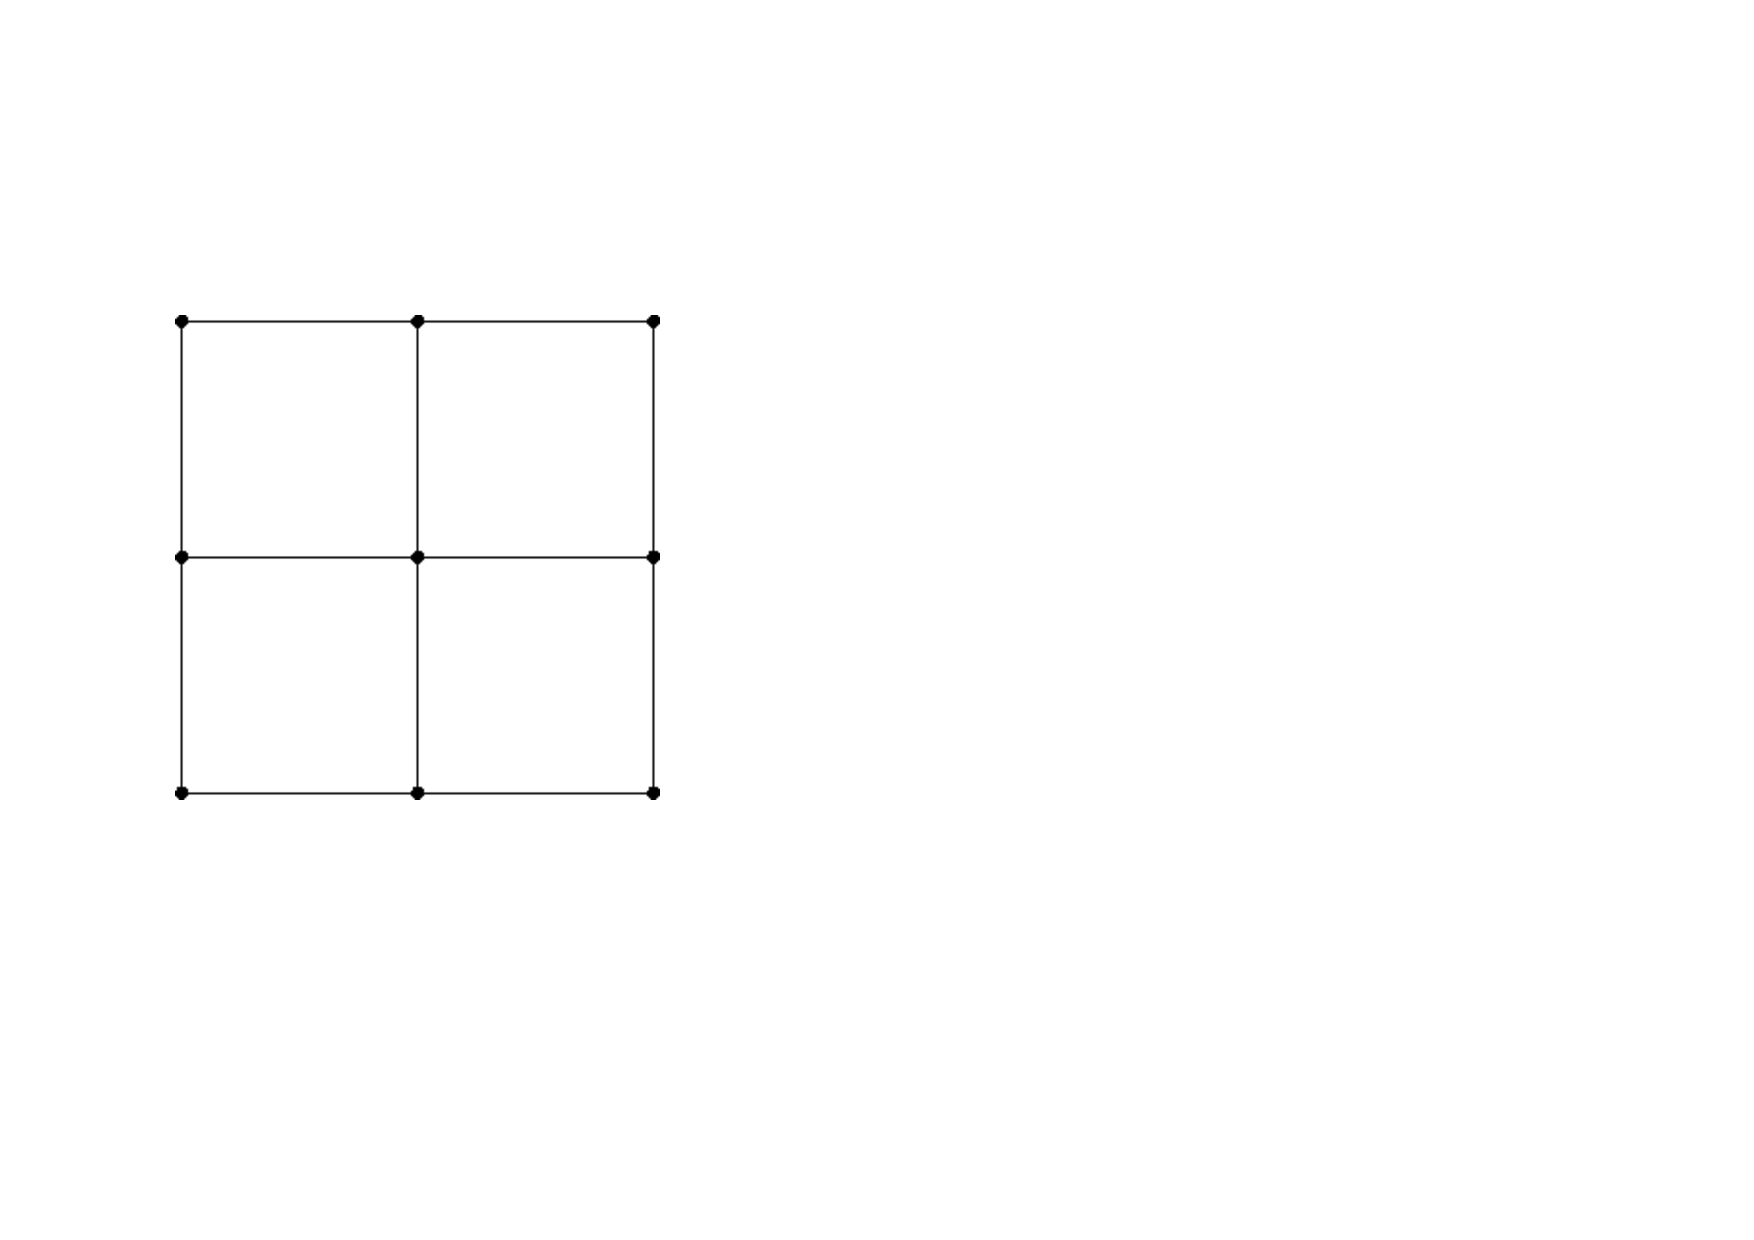
\includegraphics[width=5cm, height=5cm]{figures/coarse_mesh.pdf} 
			     \caption{}
				%\label{fig:trace1}
		\end{subfigure}
        \qquad
		\begin{subfigure}{10 cm}
				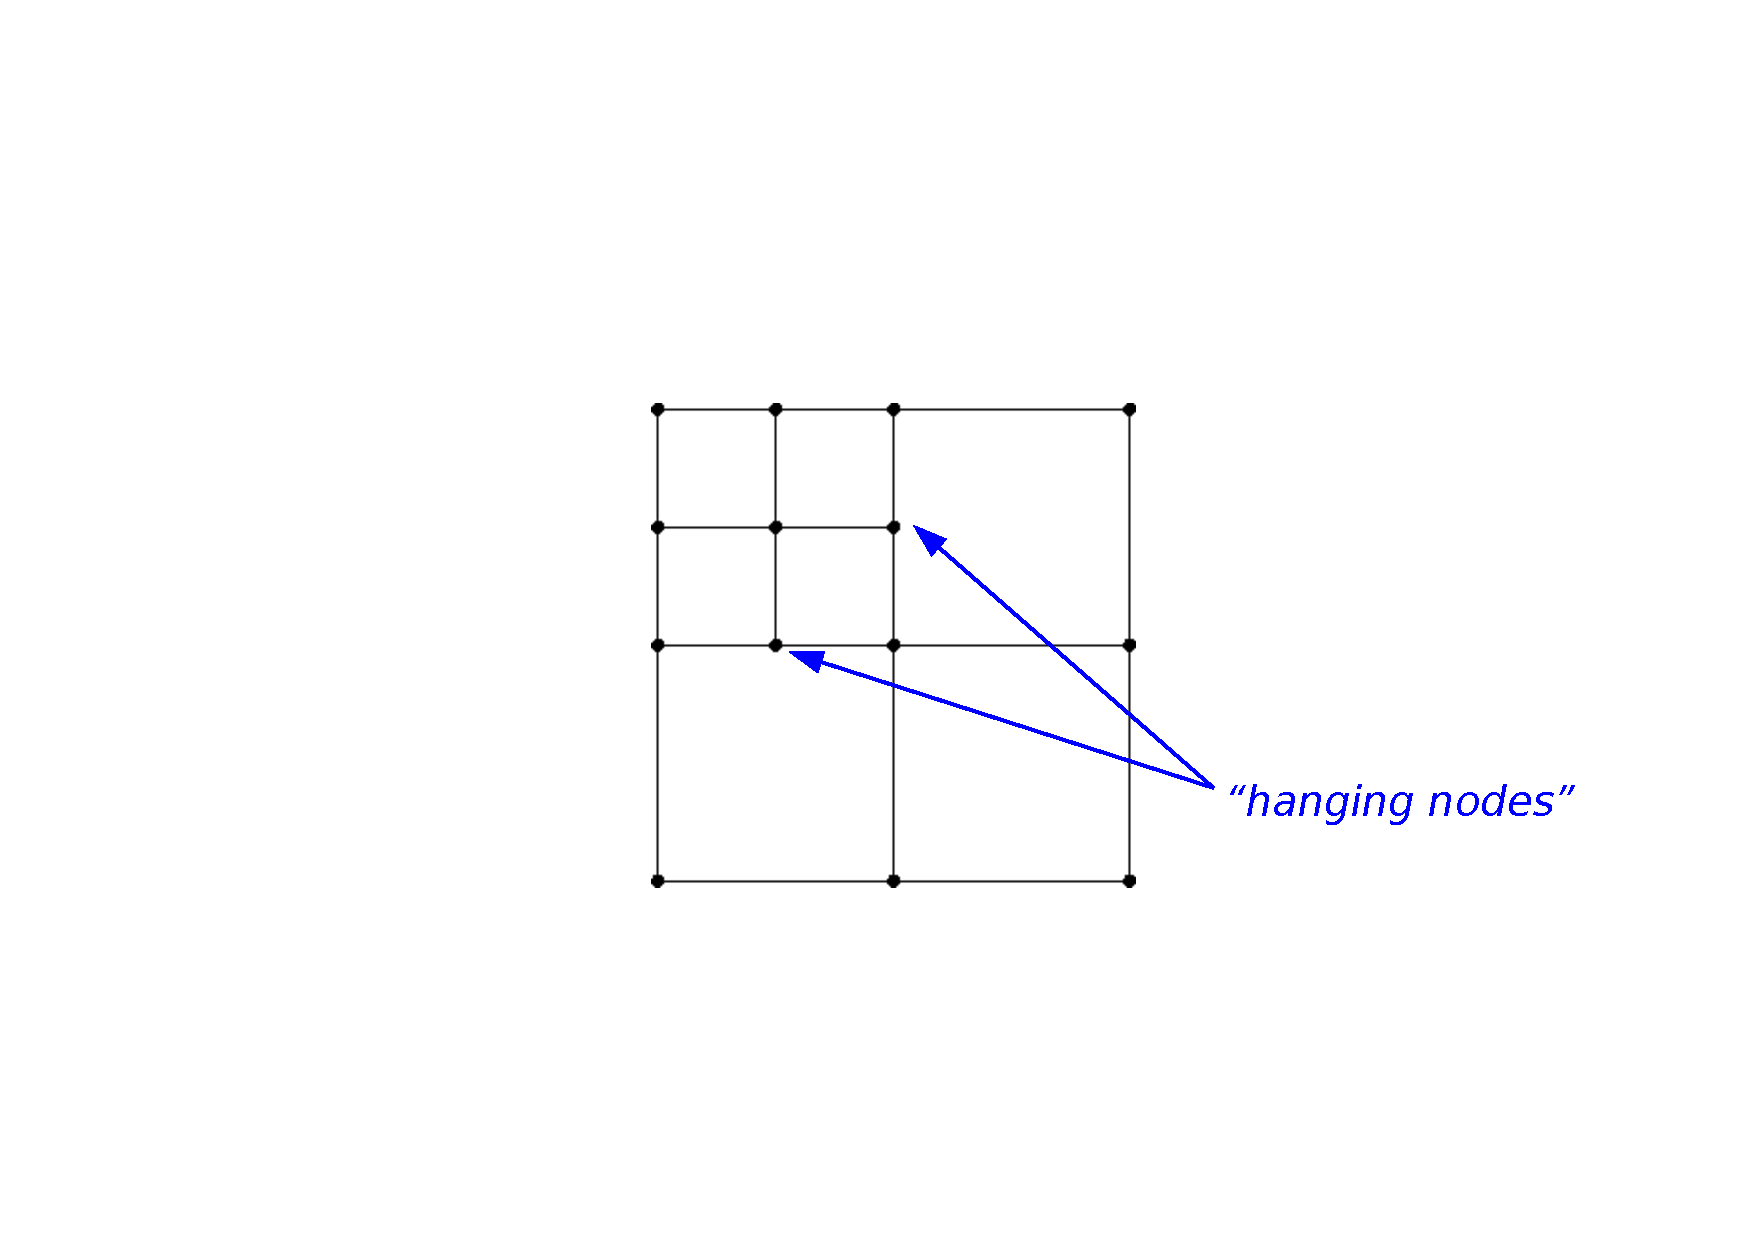
\includegraphics[width=9.2cm, height=5.3cm]{figures/mesh_hanging_nodes.pdf}
			   \caption{}
				%\label{fig:trace3}
		\end{subfigure}
 
	\caption{(a) Coarse Mesh. (b) Locally refined mesh with hanging nodes. Modified from class notes in \cite{Bangerth2013}. }
	\label{fig:2.1}
\end{figure}

\section{Time Discretization of the Weak Formulation}
For the time discretization, I subdivide  the time interval $I=(0,T]$ into sub-intervals $I_n=(t_{n-1}, t_n)$  of equal length $\Delta t =t_n-t_{n-1}$, where the discrete solution approximations for the corresponding times are $p_h^{n-1}$, $p_h^n$, and  $v_h^{n-1}$, $v_h^n$, respectively. Then, the time-discretized form of equation \ref{Eq2.4} applying the $\theta$-scheme with $\theta \in [0-1]$ is as follows:
 \begin{equation} \label{Eq2.10}
 \begin{split}
   & \left( p_h^n - p_h^{n-1},\phi_h \right)_\Omega -  \Delta t \left( \theta v_h^n + (1-\theta) v_h^{n-1}, \phi_h \right)_\Omega    =0,\\
   & \left( v_h^n-v_h^{n-1}, \phi_h \right)_\Omega  + \left(  c_b p_h^n - p_h^{n-1}, \phi_h  \right)_{\partial \Omega} + \Delta t \left( \theta c^2 \nabla p_h^n  + (1-\theta) c^2 \nabla p_h^{n-1}, \nabla \phi_h  \right)_\Omega\\
    &= \Delta t \left( \theta f^n +(1-\theta)f^{n-1}, \phi_h \right)_\Omega .
 \end{split}
 \end{equation}


\section{ Implementation}
For this work I  set $\theta =0.5$, for which the $ \theta$-method becomes the Crank-Nicholson scheme. Since I use the same mesh for every time step, the shape functions are the same for every time step as well: $\phi_h = \phi_h^n =\phi_h^{n-1} $. 
I also assume that solution vector is $D_p^n$  for $p_h$ and $D_v^n$ for $v_h$ at time $t_n$. The elements of these vectors are the DOF $D_{p_i}^n$  and $D_{v_i}^n$ at the nodes $i$. Then I can write the the solution approximation at the time step $t_n$ as:
 \begin{equation} \label{Eq2.11}
 \begin{split}
   & p_h^n=\sum_{i \in I}  D_{p_i}^n \phi_{h_i}(x),\\
   & v_h^n=\sum_{i \in I} D_{v_i}^n \phi_{h_i}(x).
 \end{split}
 \end{equation}
 
 Where, depending on the FEM approach, $\phi_{h_i}$ are either the standard FEM basis functions or the standard plus enriched basis functions. Thus, equation \ref{Eq2.11} is a generalization of equations \ref{Eq2.5} and \ref{Eq2.7}. Then, after replacing equation \ref{Eq2.11} into equation \ref{Eq2.10} and simplifying terms, I write equation \ref{Eq2.10} in matrix form as follows:
  \begin{equation} \label{Eq2.12}
 \begin{split}
   & L_p D_p^n = R_p, \\
   &L_v D_v^n = R_v.
 \end{split}
 \end{equation}
 
 Where matrices $L_p$ and  $L_v$ and vectors  $R_p$, and  $R_v$ are defined as follows:
 \begin{equation} \label{Eq2.13}
 \begin{split}
   &L_p = M + \Delta t \theta B +{\Delta t}^2 A, \\
   & L_v=M,\\
   &R_p= \left( M + \Delta t \theta B -{\Delta t}^2  \theta^2(1-\theta) A \right) D_p^{n-1}\\
   &+{\Delta t}^2  \theta^2 F^n + {\Delta t}^2 \theta F^{n-1},\\
   & R_v=M D_v^{n-1} + \left( B -  \Delta t (1-\theta) A \right) D_p^{n-1} \\
   & -\left(  B + \Delta t \theta A \right) D_p^n +\Delta t \theta F^n + \Delta t( 1- \theta) F^{n-1}.
 \end{split}
 \end{equation}
 
With matrices $M$, $A$ and $B$, and vectors $F^n$ and $F^{n-1}$ defined as:
 \begin{equation} \label{Eq2.14}
 \begin{split}
  & M_{ij}=(\phi_{h_i},\phi_{h_j})_\Omega,\\
  & A_{ij}=(c^2 \nabla \phi_{h_i},\nabla \phi_{h_j})_\Omega,\\
  & B_{ij} =(c_b  \phi_{h_i}, \phi_{h_j})_{\partial \Omega },\\
  & F_i^n = (f^n, \phi_{h_i})_\Omega,\\
  & F_i^{n-1} = (f^{n-1}, \phi_{h_i})_\Omega.\\
 \end{split}
 \end{equation}

I also define the continuous function $f (x,t)$ in a similar way as in \cite{Yue2005}:
 \begin{equation} \label{Eq2.15}
 \begin{split}
  & f(x,t) = a_o f_1(t) f_2(x),\\
  &  f_1(t) = f_o (t-t_o) \exp \left( \pi^2 f_o^2 (t-t_o)^2   \right) \quad \forall \quad t \leq t_o,\\
  & f_2(x) =\left( 1- \frac{\Vert x - r_o \Vert ^2 }{R_s^2} \right)^3 \frac{1}{V} \quad \forall \quad \Vert x-r_o \Vert \leq R_s, \\ 
  & V =\frac{\pi}{4} R_s^2.\\
 \end{split}
 \end{equation}

Where $f(x,t) =f$ is the right hand side of the PDE defined in equation \ref{Eq2.1} and represents a seismic source,  $a_o$ is a scaling factor, $f_o = 1/t_o$ is the central frequency of the source, $r_o$ is the source center, $\Vert .\Vert$ is the Euclidean distance and $R_s$ is the source radius. The spatial part of the source $f_2(x)$ is normalized by its volume $V$, so that the size of the source does not affect the wave amplitude, at least from a theoretical point of view. In a numerical implementation, however, source size might have an effect on the wave amplitude when the mesh size is not fine enough to sample the source a required number of times. I explore the source size effect in the GFEM simulations in section 3.1.1.

\subsection{Mesh Generation and Numerical Simulation}
All the software I use for this work is open source. I use \textbf{gmsh} \cite{Geuzaine2009} to generate quadrilateral meshes. The advantage of \textbf{gmsh} is that it allows for flexible meshing, generating elements that conform to complex geometry boundaries. It also has the capability to control element size in different regions of the mesh, keeping mesh regularity. I also use \textbf{tethex} (https://github.com/martemyev/tethex/wiki), which is a utility that arranges \textbf{gmsh} mesh output to a format that is compatible with the FEM library \textbf{deal.II} \cite{Bangerth2007} that I use to implement the acoustic wave simulation. \textbf{deal.II}  provides the necessary tools  for simulation with FEM, including classes that implement the standard and enriched  basis functions \cite{Davydov2017}. This library is built using object-oriented programming in C++, with modular classes that include mesh generation, definition of finite element spaces, linear solvers and post-processing capabilities among others. \textbf{deal.II} can create non-conforming locally refined meshes and has the capability to handle hanging node constraints to maintain  the continuity of  the finite element space . Although for this work I implement a continuous Galerkin formulation, \textbf{deal.II} also allows for a discontinuous Galerkin implementation.
\textbf{deal.II} implements finite element linear systems, as the ones in equation \ref{Eq2.12}, in the standard fashion, by performing calculations at each element $K$ of a mesh $\tau$. For instance:  $(.,.)_\Omega= \displaystyle\sum_{K \in \tau} (.,.)_K$.

\section{Error Estimate}
%revise this
The proposed method estimates the error between the traces obtained  using the GFEM and a reference solution, in which the reference solution results from applying the FEM in a fine mesh. For that I define an error measure $E_k$:

 \begin{equation} \label{Eq2.17}
  E_k =\left| 1 - \left|  \frac{ CC_k }{AC_0 }  \right| \right|
 \end{equation}

Where $CC_k$ is the cross correlation between the test and reference solution either for the zero lag ($k=0$) or at the maximum cross correlation value ($k=max$) and $AC_0$ is the zero lag auto correlation of the reference solution.

%%%%%%%%%%%%%%%%%%%%%%%%%%%%%%%%%%%%%%%%%%%%%%%%%%%
%
%  New template code for TAMU Theses and Dissertations starting Fall 2016.  
%
%
%  Author: Sean Zachary Roberson
%  Version 3.17.09
%  Last Updated: 9/21/2017
%
%%%%%%%%%%%%%%%%%%%%%%%%%%%%%%%%%%%%%%%%%%%%%%%%%%%
%%%%%%%%%%%%%%%%%%%%%%%%%%%%%%%%%%%%%%%%%%%%%%%%%%%%%%%%%%%%%%%%%%%%%%
%%                           SECTION III
%%%%%%%%%%%%%%%%%%%%%%%%%%%%%%%%%%%%%%%%%%%%%%%%%%%%%%%%%%%%%%%%%%%%%

\chapter{ \uppercase{Numerical Examples}}

In the following examples I explore the advantages of the GFEM approach when compared to the standard FEM regarding accuracy and simulation time for some relevant cases in exploration seismology. In these examples I use a model in $R^2$ whose dimensions are 800 m in the horizontal direction and 400 m in the vertical direction except for the last case for which I include some topographic relief. I also include a seismic source as defined in equation \ref{Eq2.15} with a central frequency $f_o=$40 Hz. For every example I find a reference solution in a fine mesh applying the standard FEM, and compare the performance against various GFEM simulation cases, presenting error estimates versus simulation time. I also find additional solutions with the standard FEM for coarser meshes to compare the overall performance against the GFEM technique. 

From the second seismic model on-wards I show the corresponding shot gathers in a variable density presentation (See Figures \ref{fig:3.15}, \ref{fig:3.27} and  \ref{fig:3.41}). For all these figures the amplitude of the traces have been modified by incorporating a time dependent divergence correction and by applying a fixed gain to each trace with the purpose of enhancing data visualization.

To find the divergence corrected traces I use the following equation:
 \begin{equation} \label{Eq3.1}
  T_d(t) = T(t)\, t^\alpha
 \end{equation}
Where  $T_d(t)$ is the divergence-corrected trace,$T(t)$ is the trace to modify, $t$ is time and $\alpha$ is a user defined factor. Since the purpose of this correction is to enhance later arrivals, $\alpha$ is commonly greater than 1.

The fixed gain is applied as follows:
 \begin{equation} \label{Eq3.2}
  Tg_i(t) = \frac{mx}{mx_i}\, T_i(t)
 \end{equation}
Where $Tg_i(t)$ is the i-th gain-modified trace of a shot gather, $Tg_i(t)$ is the corresponding input trace, $mx$ is the maximum amplitude of the shot gather and $mx_i$ is the maximum amplitude of the corresponding trace.

All other figures showing individual traces correspond to raw data without any further modification.

\section{Case 1: Homogeneous Medium}
For this case, I  assume that the medium has an acoustic velocity of 1800 m/s. I  place a seismic source at the center of the model, I also locate receivers in a radial configuration at 50 m and 100 m from the center of the source, with a receiver spacing of 5 degrees as shown in Figure \ref{fig:3.1}. The reference solution corresponds to a fine mesh with grid size $h=$1.5625 m and source radius of $2h$. For all the GFEM cases the wave number used for the plane wave enrichments is 0.14 m$^{-1}$, calculated by dividing the source radial frequency by the medium velocity.

 \begin{figure}[h!]
	\centering
	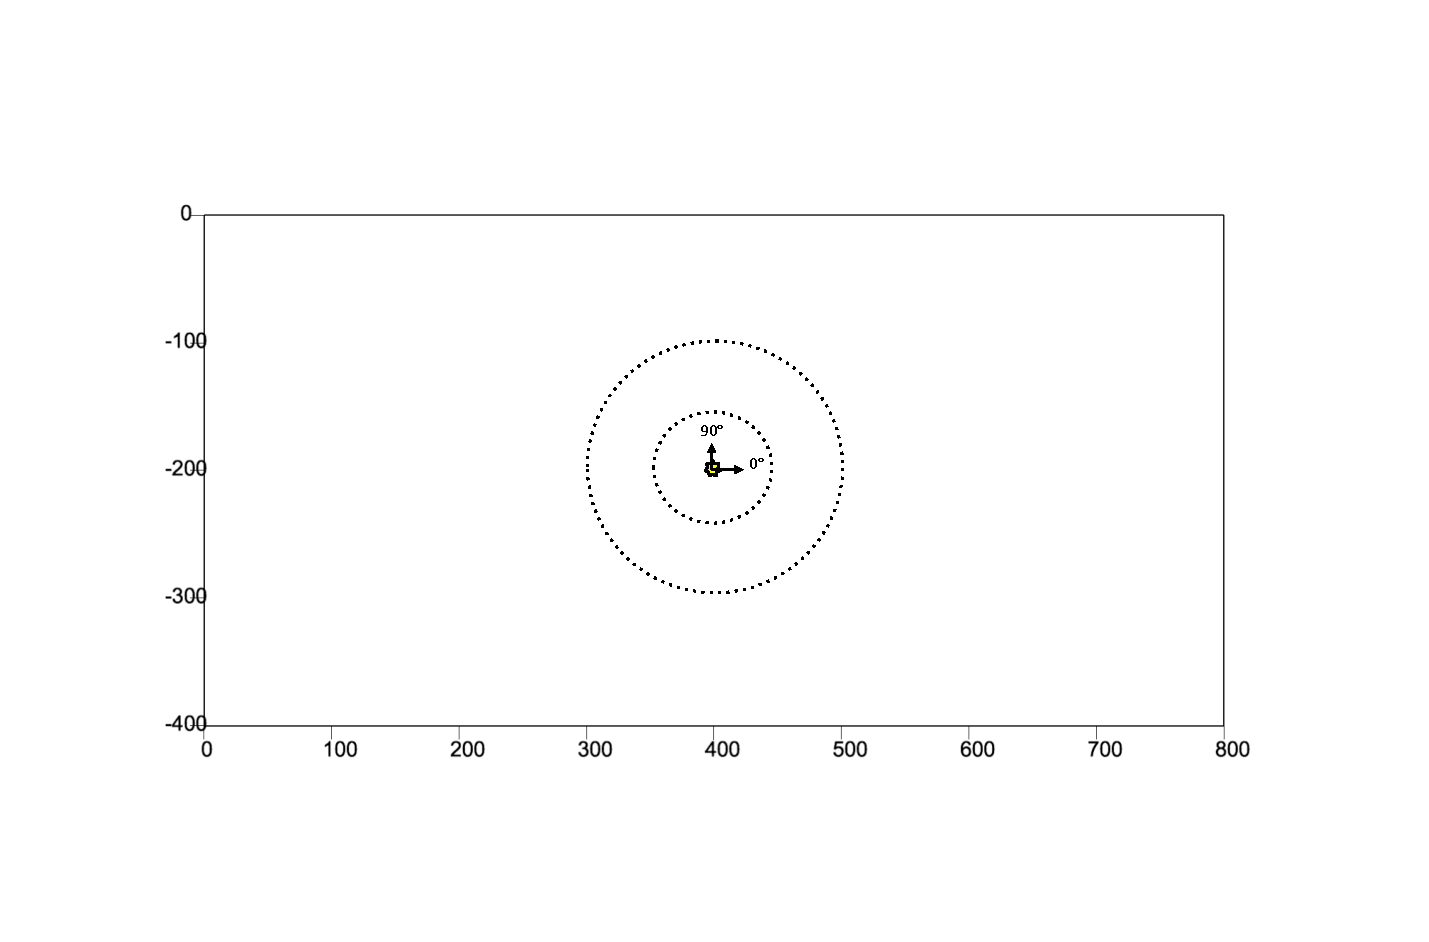
\includegraphics[width=12cm, height=6.5cm]{Thesis_Edith/figures/homo/h_source.pdf}
	\caption{Homogeneous model with a seismic source in the center (yellow star) and two sets of receiver arrays (dotted circles) at 50 m and at 100 m from the center of the source.}
	\label{fig:3.1}
\end{figure}

\clearpage
\subsection{Effect of Source Size}
%GFEM
%********************
Since I am using a source with a finite dimension for these simulations, I investigate the effect of source size on the accuracy of the GFEM solutions. Figure \ref{fig:3.2} and Figure \ref{fig:3.3} show the effect of source radius on the simulated seismograms obtained with the GFEM approach. For these cases, I used source radii equal to the mesh size and smaller than the mesh size. The plots show that to obtain the best solution approximation the source radius should be at least equal (or greater) to the mesh size as depicted in Figure \ref{fig:3.4}.

 \begin{figure}[h!]
 		\centering
		\begin{subfigure}{8cm}
				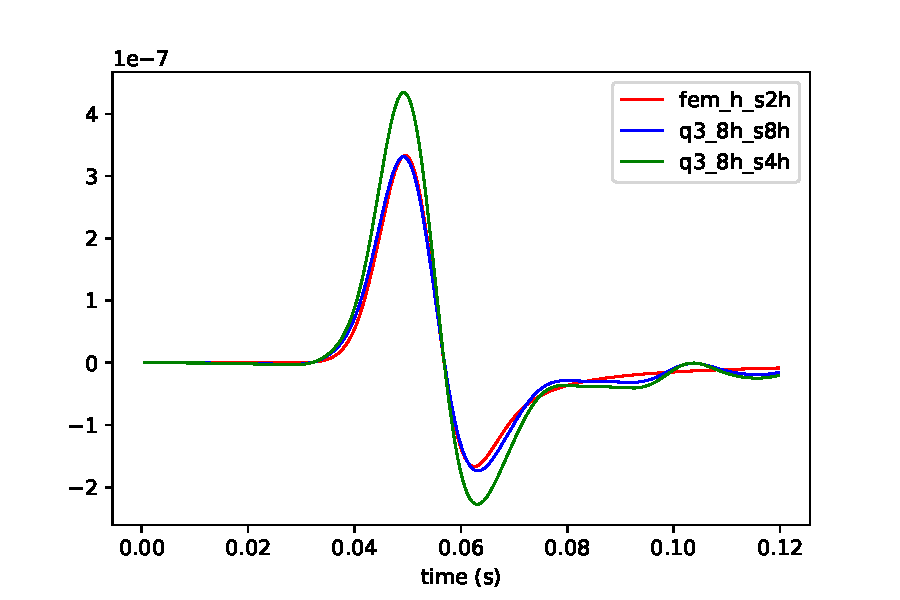
\includegraphics[width=8 cm, height=5.5cm]{Thesis_Edith/figures/homo/homo_waves/fem_q3_8h_r50_0deg.pdf} 
			     \caption{}
				%\label{fig:trace1}
		\end{subfigure}
        \hspace{0.25cm}
		\begin{subfigure}{8cm}
				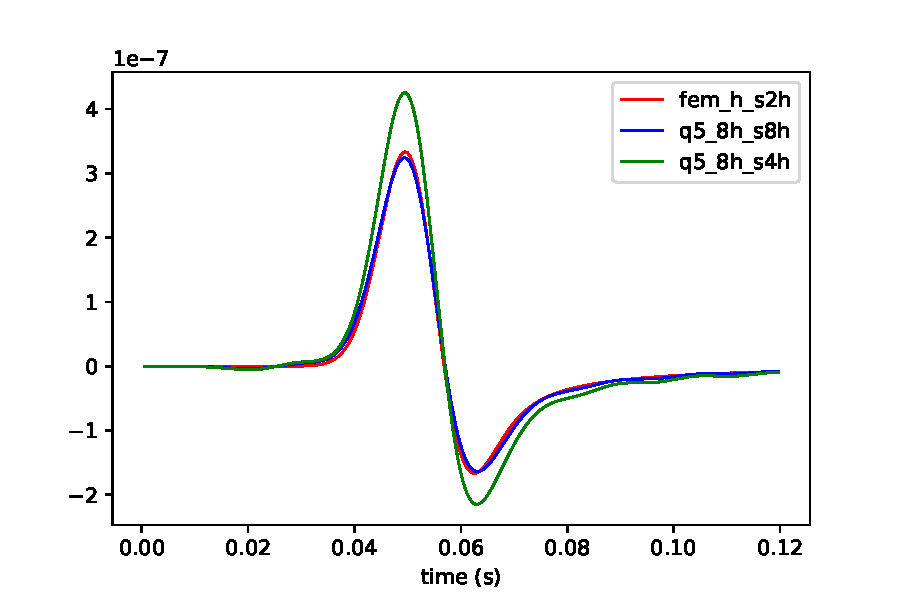
\includegraphics[width=8cm, height=5.5cm]{Thesis_Edith/figures/homo/homo_waves/fem_q5_8h_r50_0deg.pdf}
			   \caption{}
				%\label{fig:trace3}
		\end{subfigure}
 
	\caption{Homogeneous model: Seismograms for a receiver at 0 deg and  50 m from the source center  (see Figure \ref{fig:3.1}). GFEM solutions correspond to a mesh size of $8h$ and source radius of  $8h$ and $4h$. (a) Seismograms for the reference solution and 2 GFEM solutions with plane waves in 3 directions. (b) Seismograms showing the reference solution and 2 GFEM solutions with plane waves in 5 directions.}
	\label{fig:3.2}
\end{figure}


 \begin{figure}[h!]
 		\centering
		\begin{subfigure}{8cm}
				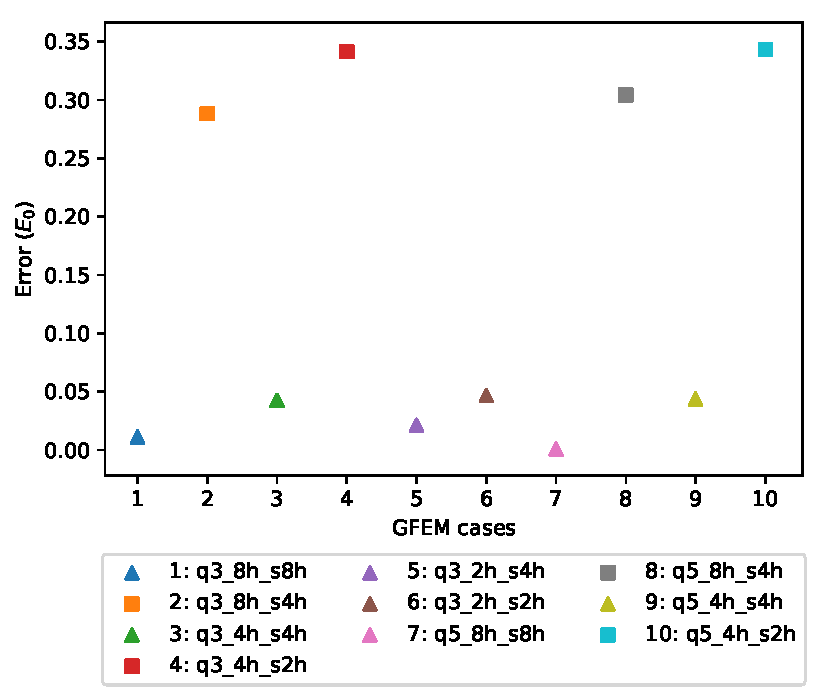
\includegraphics[width=8cm, height=6cm]{Thesis_Edith/figures/homo/homo_waves/error_gfem_50m.pdf} 
			     \caption{}
				%\label{fig:trace1}
		\end{subfigure}
        \hspace{0.25cm}
		\begin{subfigure}{8cm}
				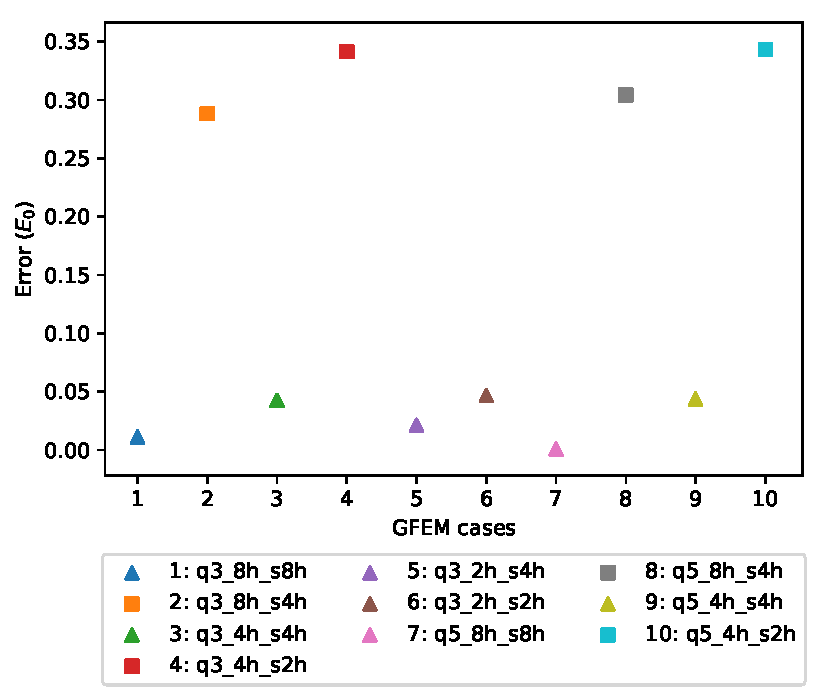
\includegraphics[width=8cm, height=6cm]{Thesis_Edith/figures/homo/homo_waves/error_gfem_50m.pdf}
			   \caption{}
				%\label{fig:trace3}
		\end{subfigure}
 
	\caption{Homogeneous model: (a) GFEM error  for all  seismograms at 50 m from the center of the source. (b) GFEM error for all seismograms at 100 m from the center of the source.}  
	\label{fig:3.3}
\end{figure}


 \begin{figure}[h!]
	\centering
	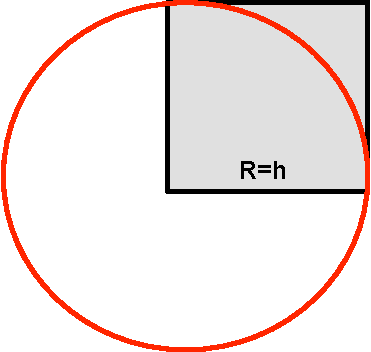
\includegraphics[width=4cm, height=4cm]{figures/source_size.pdf}
	\caption{Sketch showing the minimum source radius required according to mesh size to get a good solution approximation with the GFEM approach.}
	\label{fig:3.4}
\end{figure}

\clearpage
\subsection{Adding Refinement around the Source}
To be able to match the source size to that of the reference solution applying the GFEM  approach in a course mesh, I implement some local mesh refinement around the source location as shown in Figure \ref{fig:3.5}. Figures \ref{fig:3.6} and \ref{fig:3.7} show the seimograms for two GFEM cases in which local mesh refinement has been applied, exhibiting a good match with the reference solution. Figures \ref{fig:3.8} and \ref{fig:3.9} show the maximum cross correlation lag between GFEM solutions and the reference solution for each seismogram at 50 m from the source center, as well as two error types; one related to the maximum cross correlation ($E_{max}$) and the other one to the zero lag cross correlation ($E_0$). The lag fluctuates between -2 and 2 time steps for both GFEM cases. The observed maximum error corresponds to ($E_0$) and is around 3\%. These results show that these GFEM solutions with additional local mesh refinement around the source present an acceptable accuracy with respect to the reference solution.

% local mesh refinement around source
 \begin{figure}[h!]
	\centering
	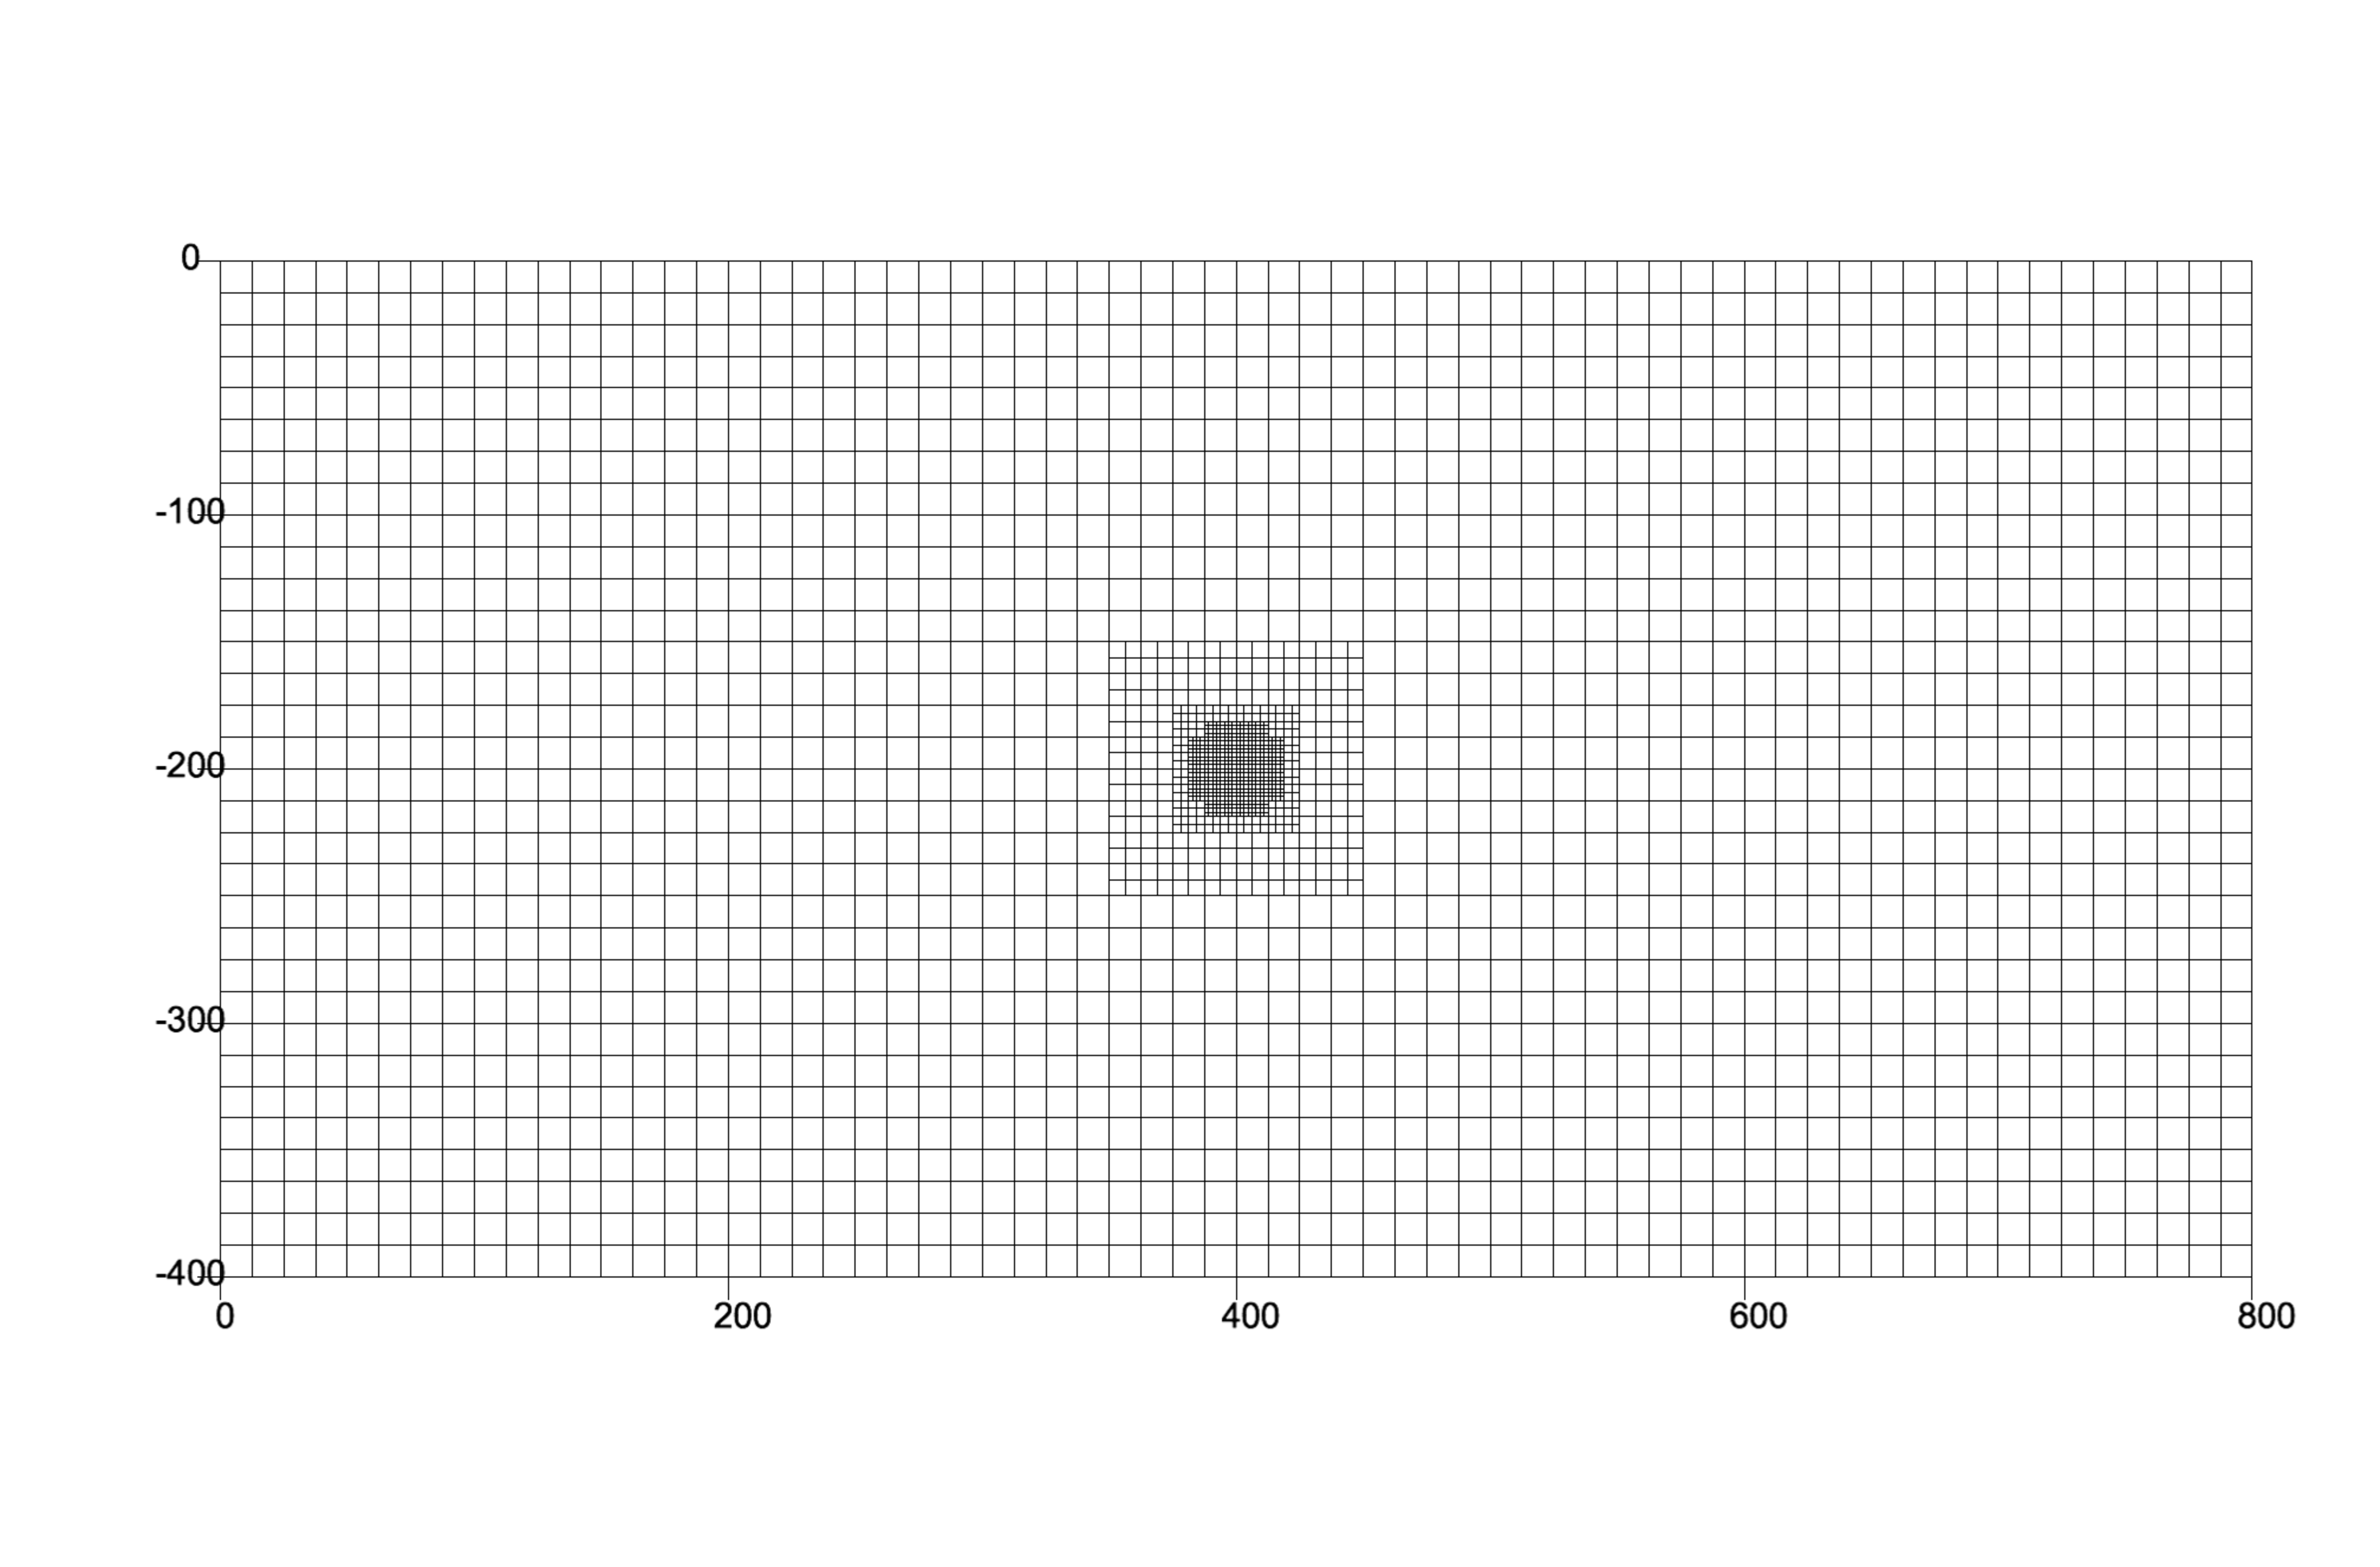
\includegraphics[width=14cm, height=7cm]{Thesis_Edith/figures/homo/h_source_doubleRef2.pdf}
	\caption{Coarse mesh with grid size of $8h$ used for GFEM simulations showing local mesh refinement around the source location.}
	\label{fig:3.5}
\end{figure}

% GFEM seismogram at 50 m from source
 \begin{figure}[h!]
 		\centering
		\begin{subfigure}{8cm}
				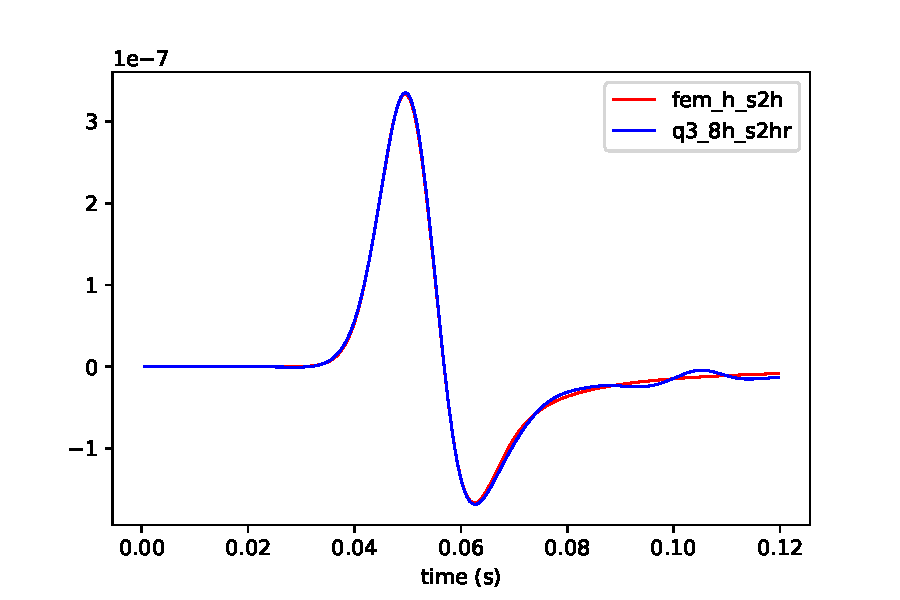
\includegraphics[width=8cm, height=6cm]{Thesis_Edith/figures/homo/homo_waves/fem_q3_8h_2hr_r50_0deg.pdf}
			     \caption{}
				%\label{fig:trace1}
		\end{subfigure}
        \hspace{0.25cm}
		\begin{subfigure}{8cm}
				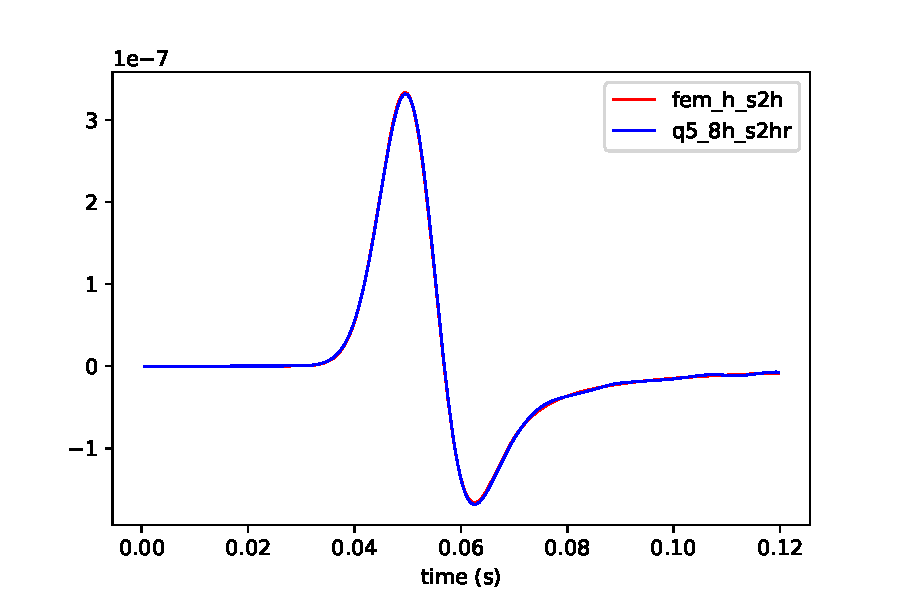
\includegraphics[width=8cm, height=6cm]{Thesis_Edith/figures/homo/homo_waves/fem_q5_8h_2hr_r50_0deg.pdf}
			   \caption{}
				%\label{fig:trace3}
		\end{subfigure}
 
	\caption{Homogeneous model: Seismograms for a receiver at 0 deg. and 50 m from the source center (see Figure \ref{fig:3.1}). GFEM solutions correspond to a mesh size of $8h$ and source radius of $2h$. (a) Seismograms for the reference solution and GFEM solution with plane waves in 3 directions. (b) Seismograms for the  reference solution and GFEM solution with plane waves in 5 directions.}  
	\label{fig:3.6}
\end{figure}

% GFEM seismogram at 100 m from source

 \begin{figure}[h!]
 		\centering
		\begin{subfigure}{8cm}
				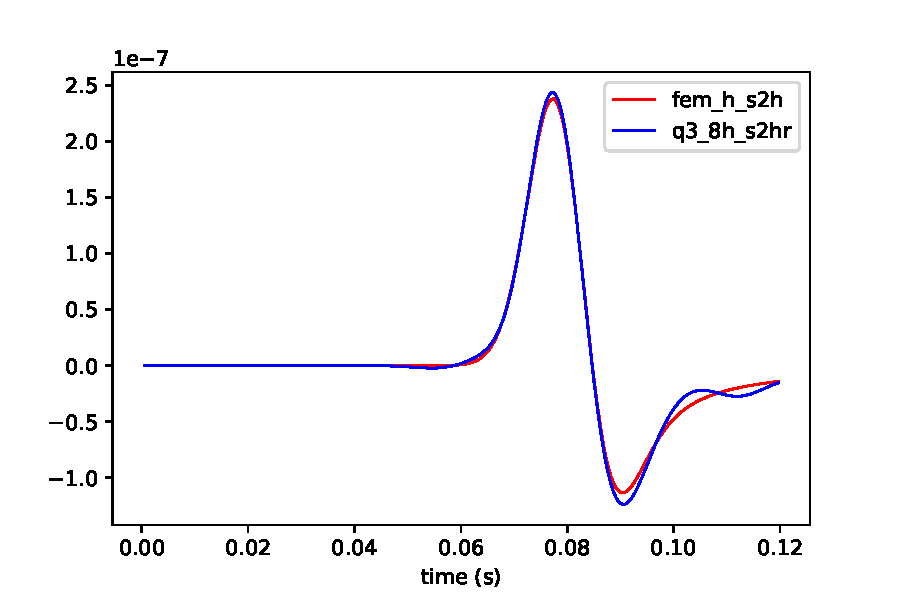
\includegraphics[width=8cm, height=6cm]{Thesis_Edith/figures/homo/homo_waves/fem_q3_8h_2hr_r100_0deg.pdf}
			     \caption{}
				%\label{fig:trace1}
		\end{subfigure}
        \hspace{0.25cm}
		\begin{subfigure}{8cm}
				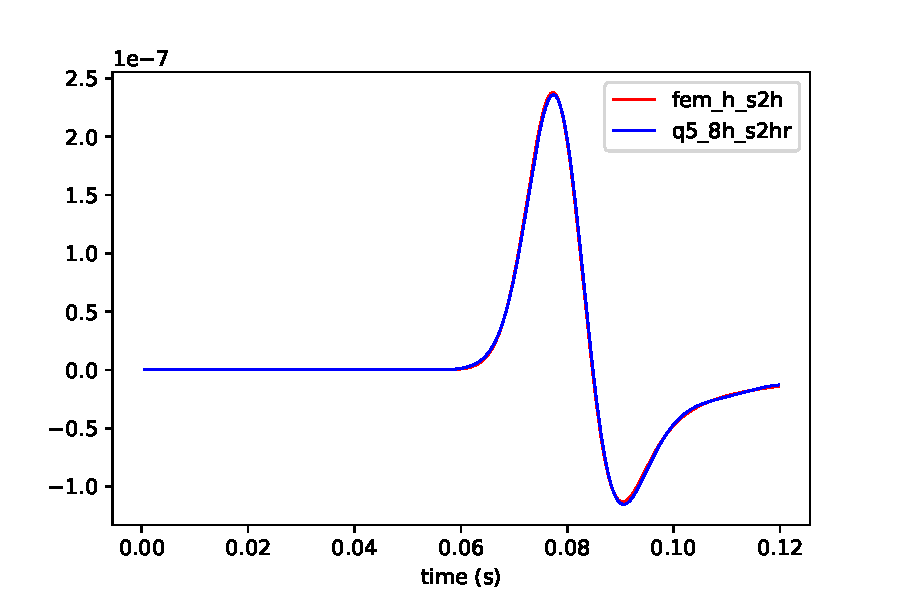
\includegraphics[width=8cm, height=6cm]{Thesis_Edith/figures/homo/homo_waves/fem_q5_8h_2hr_r100_0deg.pdf}
			   \caption{}
				%\label{fig:trace3}
		\end{subfigure}
 
	\caption{Homogeneous model: Seismograms for a receiver at 0 deg. and 100 m from the source center (see Figure \ref{fig:3.1}). GFEM solutions correspond to a mesh size of $8h$ and source radius of $2h$. (a) Seismograms for the reference solution and GFEM solution with plane waves in 3 directions. (b) Seismograms for the  reference solution and GFEM solution with plane waves in 5 directions.}  
	\label{fig:3.7}
\end{figure}

% GFEM Error @50m
 \begin{figure}[h!]
 		\centering
		\begin{subfigure}{8cm}
				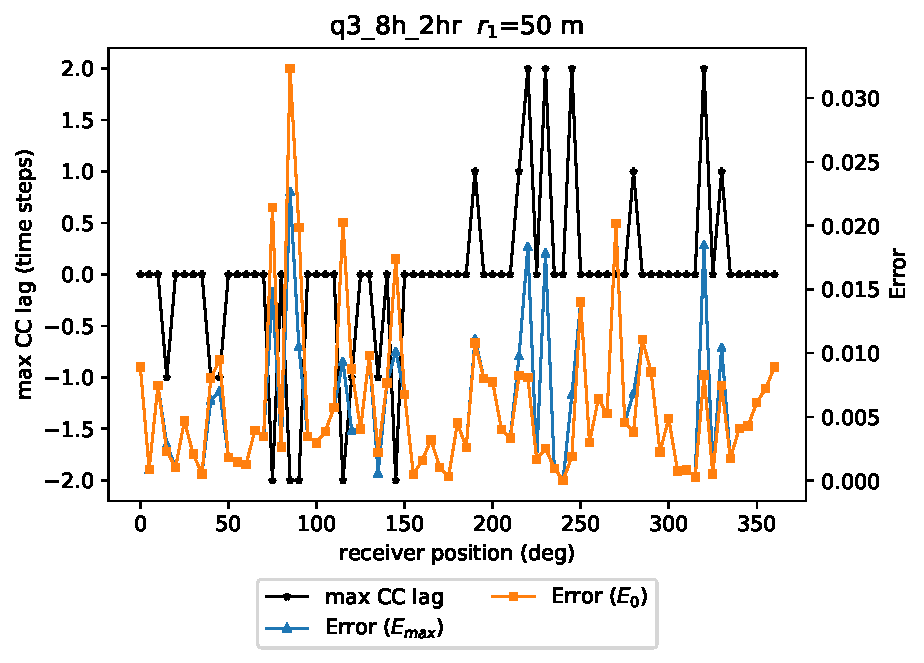
\includegraphics[width=8cm, height=6cm]{Thesis_Edith/figures/homo/homo_waves/Err_q3_8h_2hr_50m.pdf}
			     \caption{}
				%\label{fig:trace1}
		\end{subfigure}
        \hspace{0.25cm}
		\begin{subfigure}{8cm}
				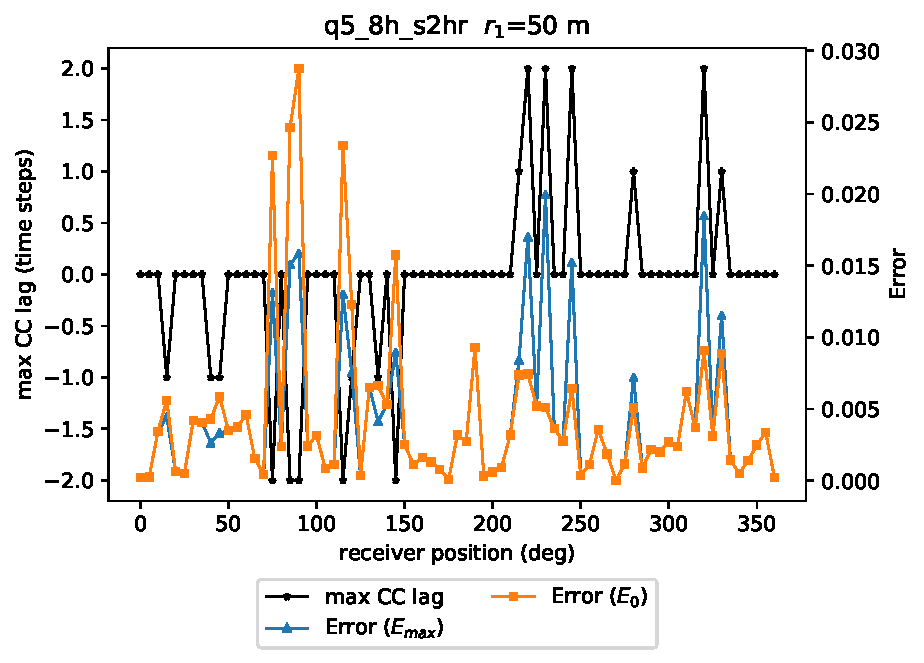
\includegraphics[width=8cm, height=6cm]{Thesis_Edith/figures/homo/homo_waves/Err_q5_8h_s2hr_50m.pdf}
			   \caption{}
				%\label{fig:trace3}
		\end{subfigure}
 
	\caption{Homogeneous model: Maximum cross correlation lag and errors for each receiver seismogram at 50 m from the source center for 2 GFEM cases with mesh size $8h$ and source size $2h$. (a) For the GFEM solution with 3 plane wave directions. (b) For the GFEM solution with 5 plane wave directions.}  
	\label{fig:3.8}
\end{figure}

% GFEM error @ 100 m
 \begin{figure}[h!]
 		\centering
		\begin{subfigure}{8cm}
				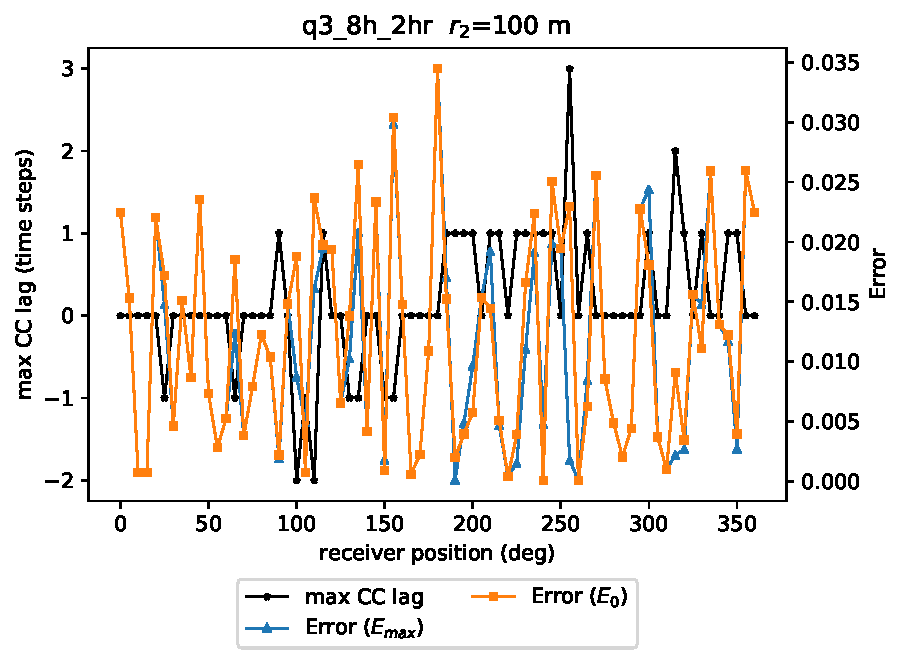
\includegraphics[width=8cm, height=6cm]{Thesis_Edith/figures/homo/homo_waves/Err_q3_8h_2hr_100m.pdf}
			     \caption{}
				%\label{fig:trace1}
		\end{subfigure}
        \hspace{0.25cm}
		\begin{subfigure}{8cm}
				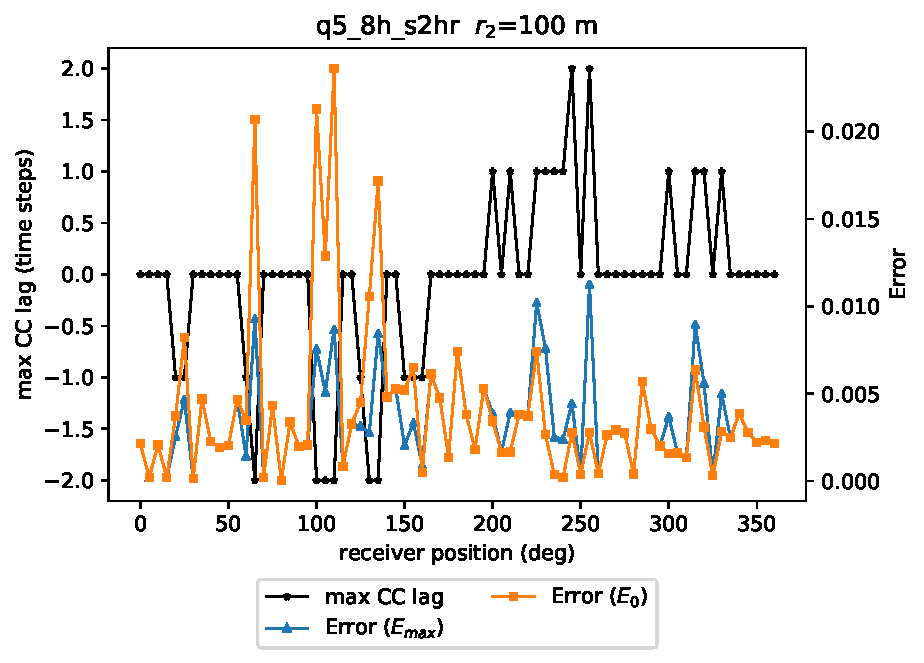
\includegraphics[width=8cm, height=5.5cm]{Thesis_Edith/figures/homo/homo_waves/Err_q5_8h_s2hr_100m.pdf}
			   \caption{}
				%\label{fig:trace3}
		\end{subfigure}
 
	\caption{Homogeneous model: Maximum cross correlation lag and errors for each receiver seismogram at 100 m from the source center for 2 GFEM cases with mesh size $8h$ and source size $2h$. (a) For the GFEM solution with 3 plane wave directions. (b) For the GFEM solution with 5 plane wave directions.}  
	\label{fig:3.9}
\end{figure}

\clearpage
\subsection{Performance Comparison}
To compare the accuracy and performance of GFEM solutions, I include two additional standard FEM solutions. Figure \ref{fig:3.10} shows the seismograms at 50 m and 100 m from the source center for two FEM solutions with coarser meshes than the reference solution. Figure \ref{fig:3.11} and \ref{fig:3.12} show the corresponding maximum cross correlation lag and errors. These results reveal that the solution accuracy deteriorates as the mesh size increases and in general the errors are greater than the GFEM cases with additional mesh refinement.

% fem seismograms
 \begin{figure}[h!]
 		\centering
		\begin{subfigure}{8cm}
				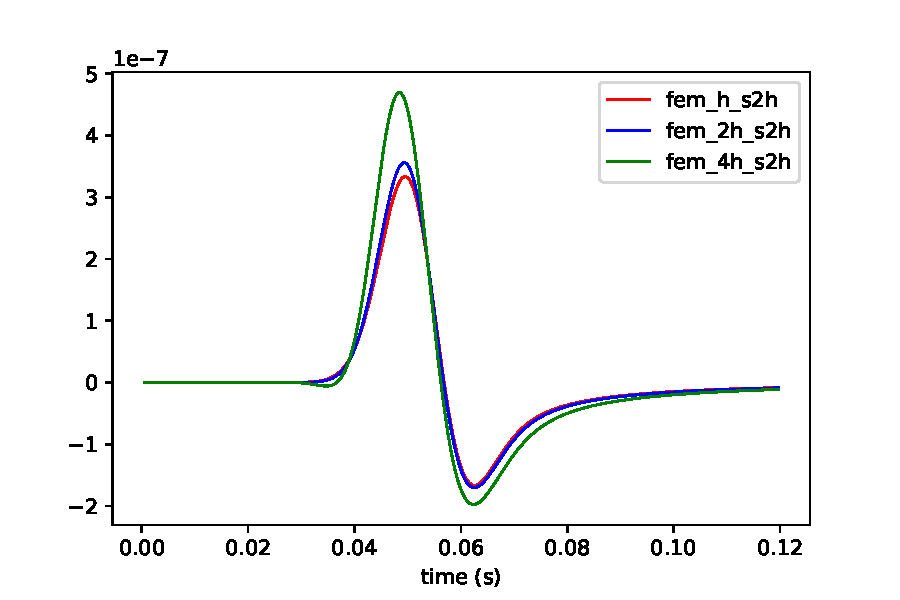
\includegraphics[width=8cm, height=6cm]{Thesis_Edith/figures/homo/homo_waves/fem_r50_0deg.pdf}
			     \caption{}
				%\label{fig:trace1}
		\end{subfigure}
        \hspace{0.25cm}
		\begin{subfigure}{8cm}
				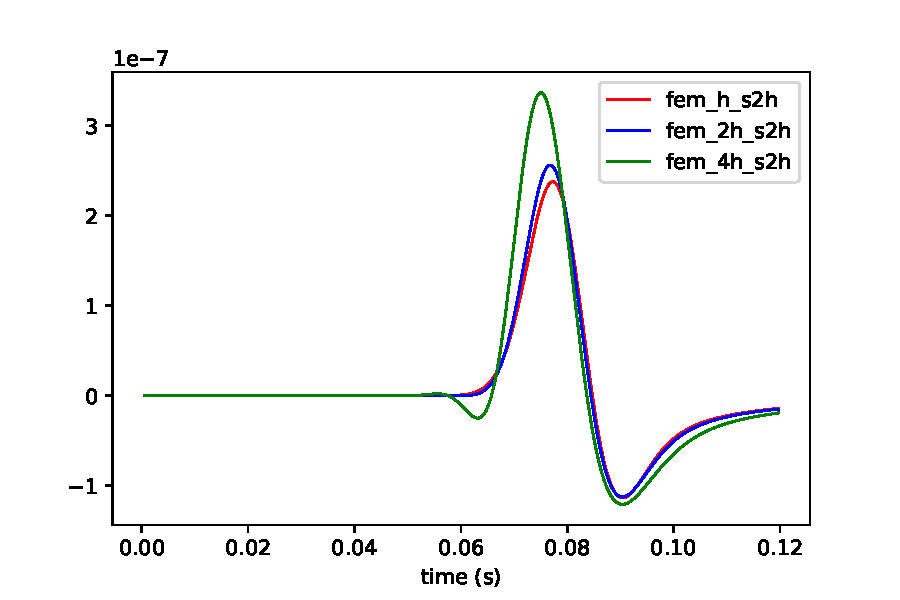
\includegraphics[width=8cm, height=6cm]{Thesis_Edith/figures/homo/homo_waves/fem_r100_0deg.pdf}
			   \caption{}
				%\label{fig:trace3}
		\end{subfigure}
 
	\caption{Homogeneous model: Seismograms for the reference solution and two additional FEM solutions with mesh size $2h$ and $4h$. (a) Seismograms at 0 deg and 50 m from the source center. (b) Seismograms at 0 deg and 100 m from the source center.}  
	\label{fig:3.10}
\end{figure}

% fem errorrs
 \begin{figure}[h!]
 		\centering
		\begin{subfigure}{8cm}
				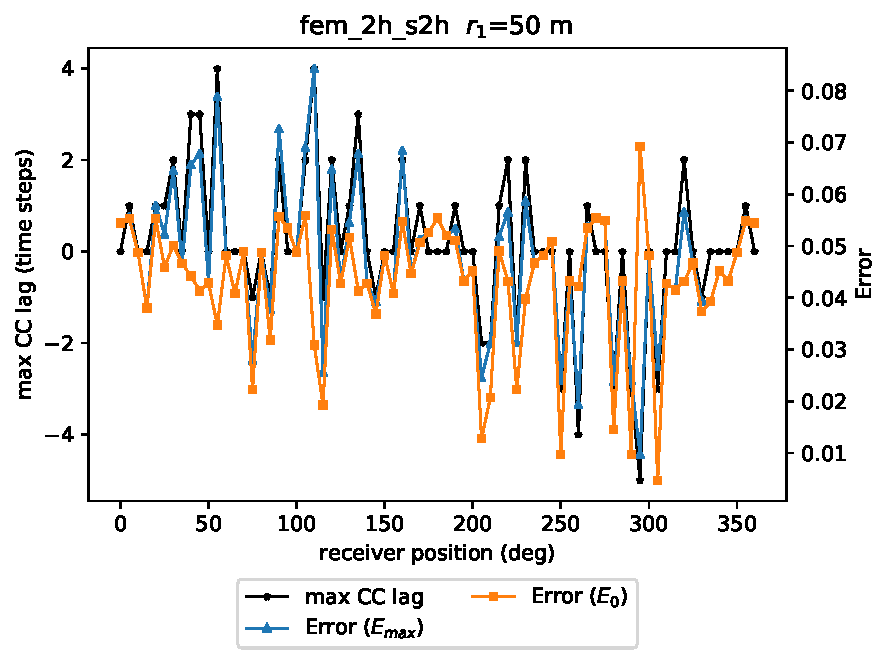
\includegraphics[width=8cm, height=6cm]{Thesis_Edith/figures/homo/homo_waves/Err_fem_2h_s2h_50m.pdf}
			     \caption{}
				%\label{fig:trace1}
		\end{subfigure}
        \hspace{0.25cm}
		\begin{subfigure}{8cm}
				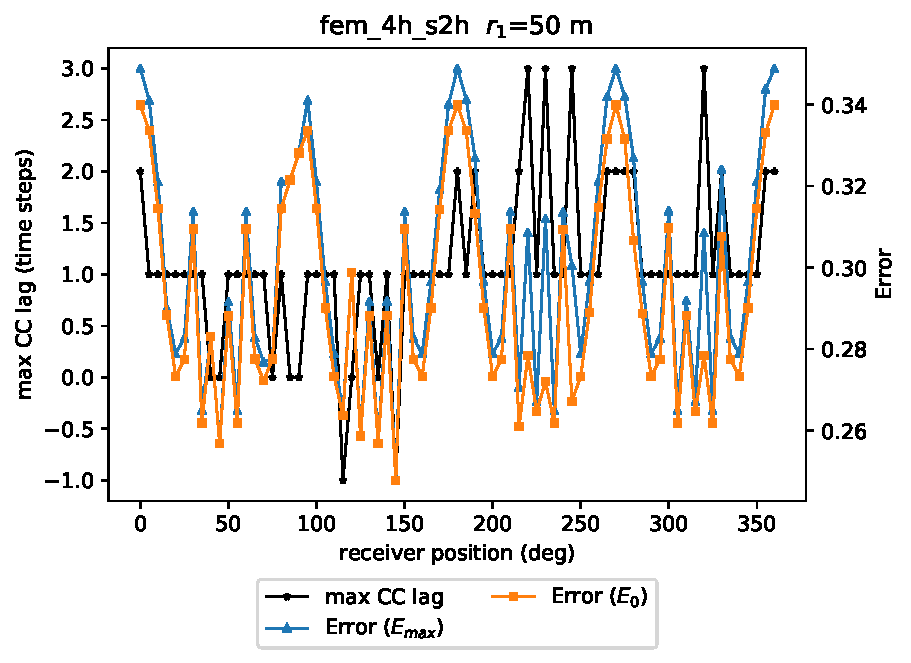
\includegraphics[width=8cm, height=6cm]{Thesis_Edith/figures/homo/homo_waves/Err_fem_4h_s2h_50m.pdf}
			   \caption{}
				%\label{fig:trace3}
		\end{subfigure}
 
	\caption{Homogeneous model: Maximum cross correlation lag and errors for seismograms for each receiver at 50 m from the source center for 2 FEM cases. (a) For the FEM solution with mesh size of $2h$. (b) For the FEM solution with mesh size of $4h$.}  
	\label{fig:3.11}
\end{figure}

 \begin{figure}[h!]
 		\centering
		\begin{subfigure}{8cm}
				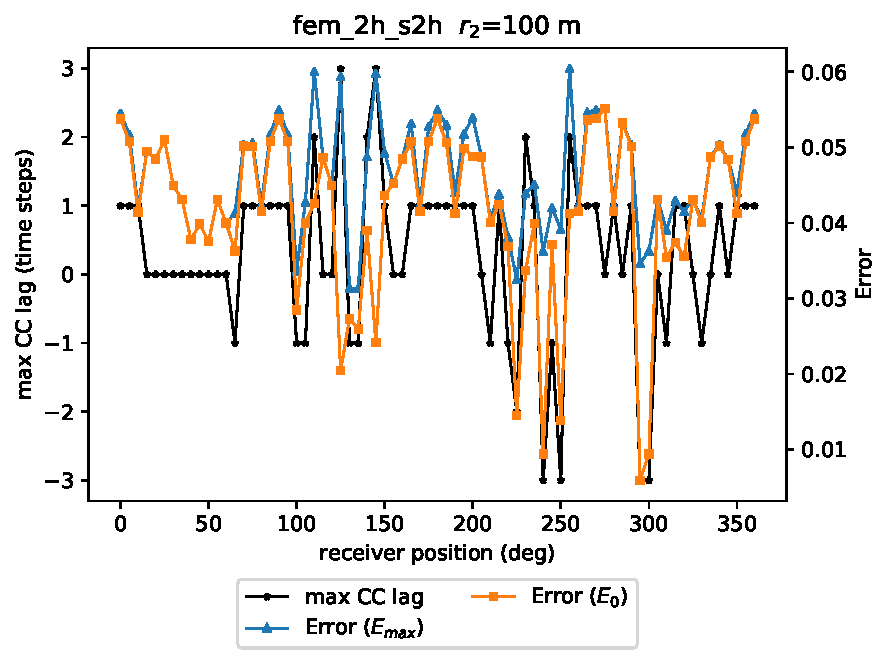
\includegraphics[width=8cm, height=6cm]{Thesis_Edith/figures/homo/homo_waves/Err_fem_2h_s2h_100m.pdf}
			     \caption{}
				%\label{fig:trace1}
		\end{subfigure}
        \hspace{0.25cm}
		\begin{subfigure}{8cm}
				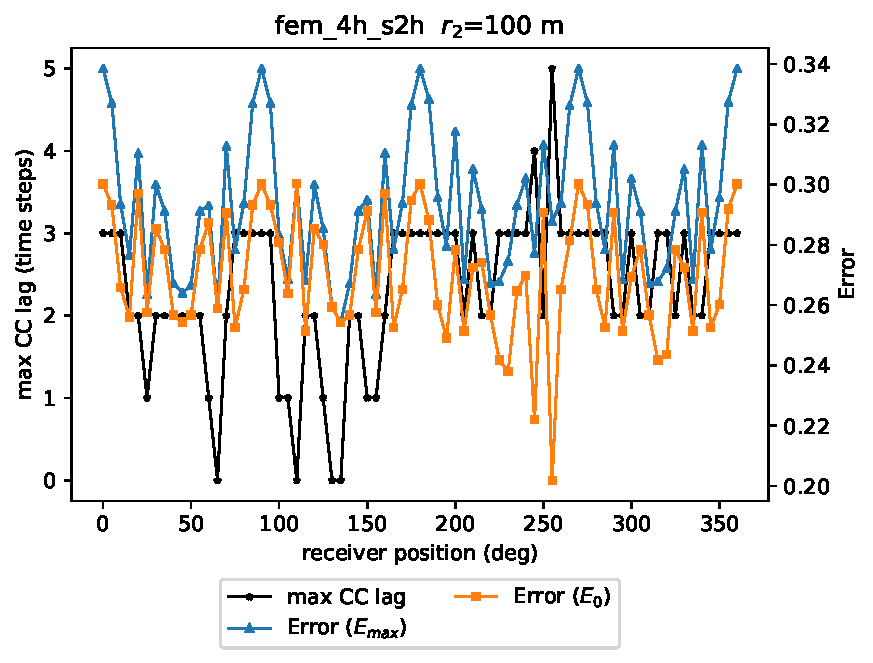
\includegraphics[width=8cm, height=6cm]{Thesis_Edith/figures/homo/homo_waves/Err_fem_4h_s2h_100m.pdf}
			   \caption{}
				%\label{fig:trace3}
		\end{subfigure}
 
	\caption{Homogeneous model: Maximum cross correlation lag and errors for seismograms for each receiver at 100 m from the source center for 2 FEM cases (a) For the FEM solution with mesh size of $2h$. (b) For the FEM solution with mesh size of $4h$.}  
	\label{fig:3.12}
\end{figure}

Figure \ref{fig:3.13} shows the the mean error versus relative simulation time and standard deviation for the additional standard FEM solutions and for various GFEM cases. the  GFEM cases correspond to  solutions with a coarse mesh  of $8h$ and with a source radius of $8h$ and $2h$. An additional GFEM result with mesh and source radius size of $4h$ is also presented. The relative simulation time were calculated as a ratio taken with respect to the reference FEM solution and the mean error is the mean of all seismogram errors at 50 and 100 m from the center of the source. For all the GFEM results, except for the case of mesh size $4h$ and plane waves in 3 directions (q3\_4h\_4h), the mean error is lower than any of the two additional FEM cases. Among The GFEM cases, the examples with the additional mesh refinement exhibit the least error and standard deviation. The GFEM solutions also present a faster simulation time than the reference solution, it is around 0.2 times the reference solution. 

% Mean error
 \begin{figure}[h!]

		\begin{subfigure}{8cm}
				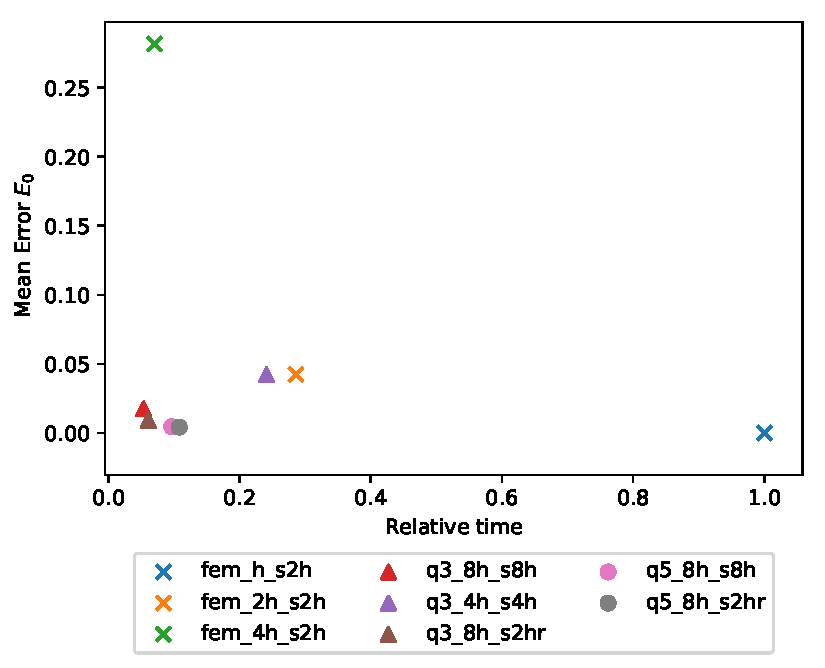
\includegraphics[width=8cm, height=6cm]{Thesis_Edith/figures/homo/homo_waves/MeanError_time_radial.pdf}
			   \caption{}
				%\label{fig:3.7b}
	    \hspace{0.25cm}	
		\end{subfigure}
				\begin{subfigure}{8cm}
				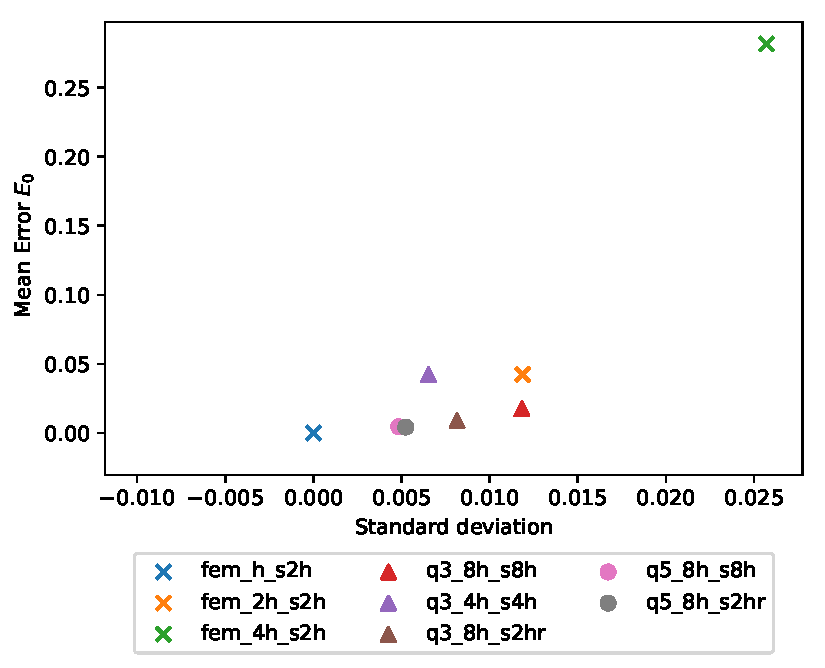
\includegraphics[width=8cm, height=6.3cm]{Thesis_Edith/figures/homo/homo_waves/Error_std_radial.pdf}
				\caption{}
				%\label{fig:3.7b}
		\end{subfigure}
 
	\caption{Homogeneous model: Mean error vs relative time and standard deviation for various FEM and GFEM cases. (a) Mean error vs relative time. (b) Mean error vs standard deviation}
	\label{fig:3.13}
\end{figure}

% New section: Layered Model
\section{Case 2: Layered Medium with Low Velocity Layer}
 The model for this example is as shown in Figure \ref{fig:3.14}, where $h_i$  and $v_i$ are the thickness and acoustic velocity of $i-th$ layer respectively. Notice that in this case the top layer presents a relative low velocity respect to the other two.  The source is located at a depth of - 50m and and at 400 m in the horizontal coordinate. There are also 50 receivers spanning from 400 m, directly above from the source, to 750 m in the horizontal coordinate very close to surface. For this case, I also find a FEM reference solution in a fine mesh of size $h$ with source radius of $2h$. I find as well 2 additional FEM solutions in mesh sizes of $2h$ and $4h$. I also obtain GFEM solutions in a coarse mesh of $8h$ and source sizes of  $8h$ and $2h$.  For all the GFEM cases the wave number used for the plane wave enrichments is 0.14 m$^{-1}$, calculated by dividing the source radial frequency by the lowest velocity (1800 m/s).
 
 Table \ref{table:3.1} shows the wavelength and wavenumber for the different layers according to their velocity. It also shows the number of cells per wavelength for the different meshes used.   
 Figure \ref{fig:3.15} shows the seismograms for the reference solution for the shot gather configuration of Figure \ref{fig:3.14}.
 
 \begin{figure}[h!]
	\centering
	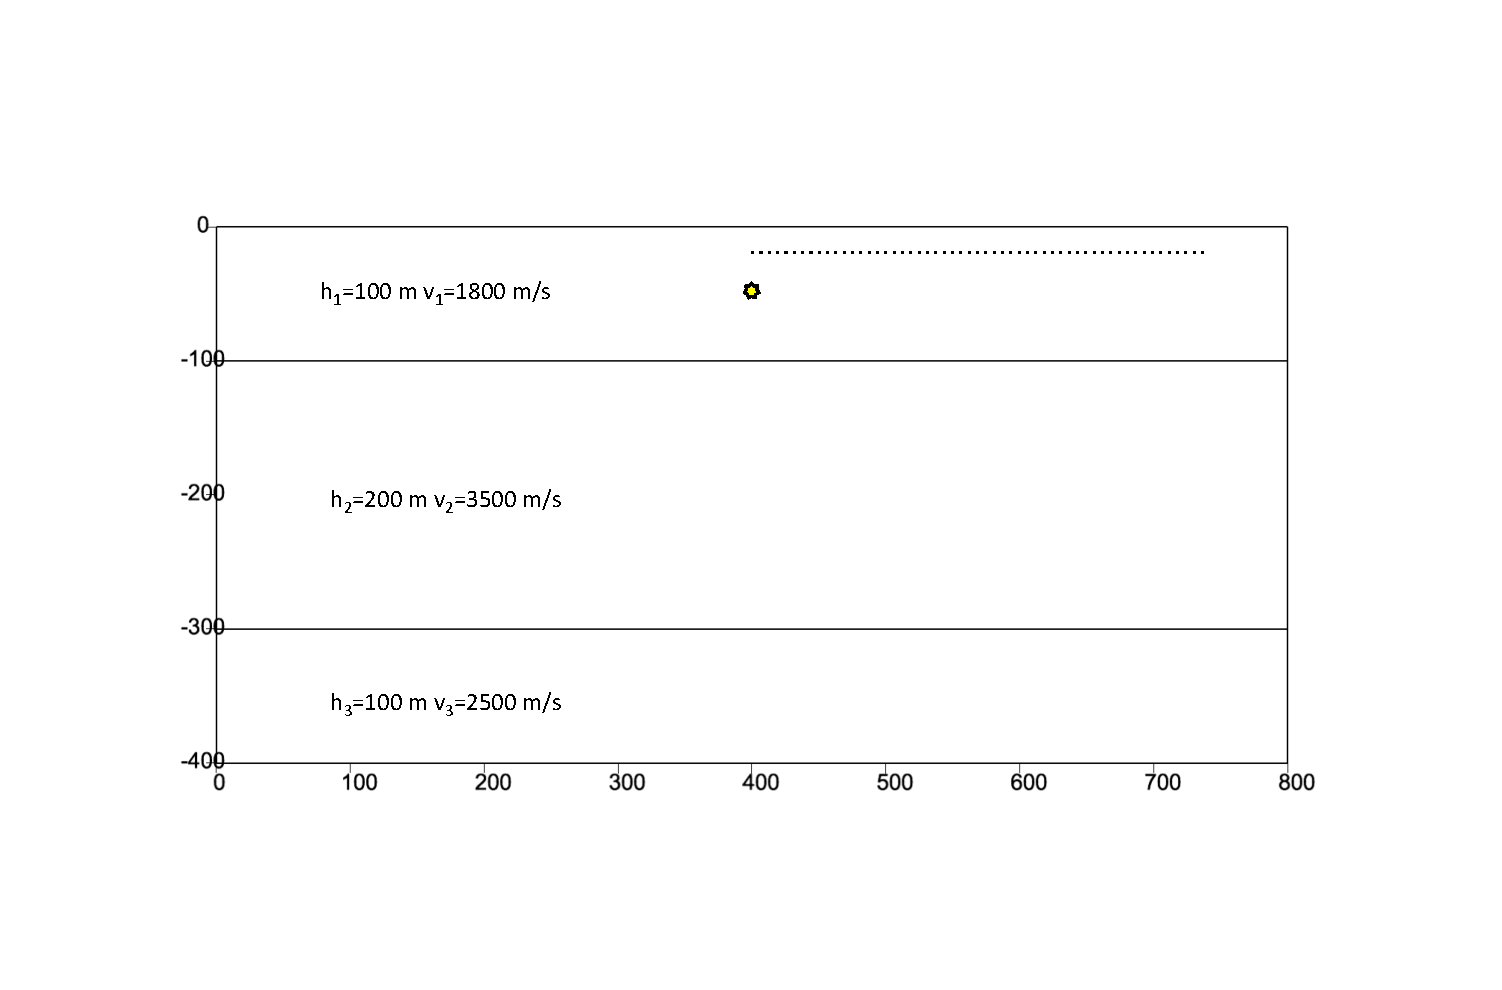
\includegraphics[width=14cm, height=7cm]{Thesis_Edith/figures/layered_model/layer_source.pdf}
	\caption{Three-layer model  with a seismic source in the first layer (yellow star) and a horizontal array of 50 receivers close to surface as depicted by the dotted line.}
	\label{fig:3.14}
\end{figure}

%table
\begin{table}[h!]
\footnotesize
\centering
    \begin{tabular}{|c|m{2cm}|m{2cm}|m{2cm}| m{1cm}|m{1cm}|m{1cm}|m{1cm}|}
      \hline
      \multirow{2}{*}{Layer} &
      \multirow{2}{2cm}{Velocity (m/s)} &
      \multirow{2}{2cm}{Wavelength \quad $\lambda$ (m)} &
      \multirow{2}{2cm}{Wavenumber  k (m$^{-1}$)} &
         \multicolumn{4}{m{4cm}|}{Number cells per wavelength in a mesh size of:} \\
         & & & & $h$ & $2h$ & $4h$ & $8h$ \\
      \hline
      1 & 1800 & 45 & 0.14 & 28.8 & 14.4 & 7.2 & 3.6\\
      \hline
      2 & 3500 & 87.5 & 0.07 & 56 & 28 & 14 & 7\\
      \hline
      3 & 2500 & 62.5 & 0.10 & 40 & 20 & 10 & 5\\
      \hline
    \end{tabular}
    \caption{Layered model: Table showing the velocity, wavelength and wavenumber for each layer, as well as the number of cells per wavelength in different mesh sizes. Source frequency is 40 Hz and $h=$1.5625 m}
    \label{table:3.1}
\end{table}

%shot gather
 \begin{figure}[h!]
	\centering
	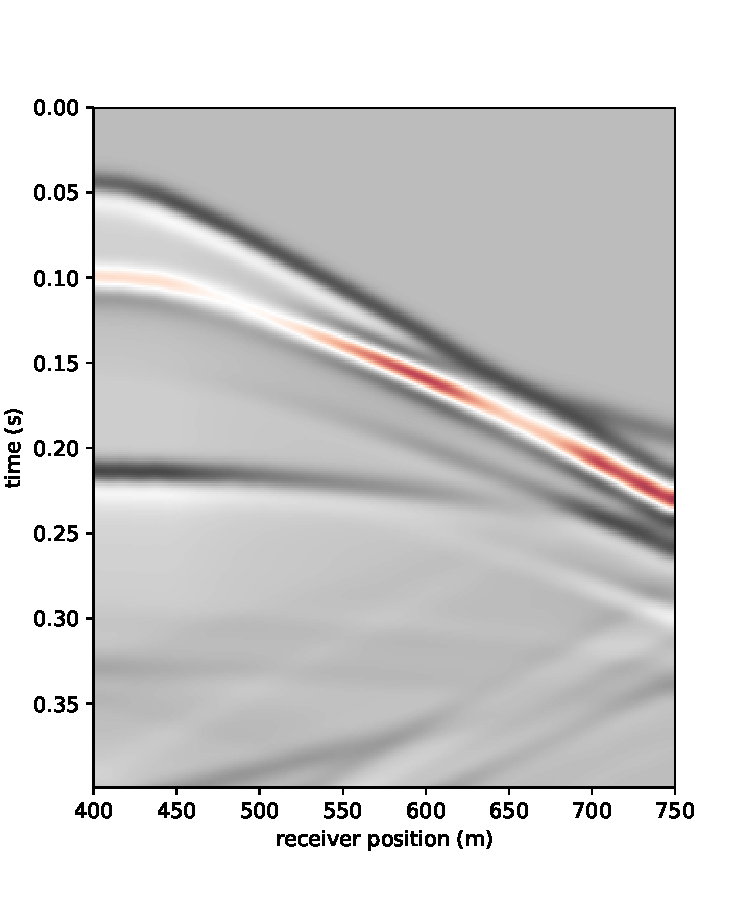
\includegraphics[width=10cm, height=13cm]{Thesis_Edith/figures/layered_model/layer_waves/seismogram_layered.pdf}
	\caption{Layered model: Seismograms of the shot gather as depicted in Figure \ref{fig:3.14} of the reference solution. Coefficient for the divergence correction is 2.5.}
	\label{fig:3.15}
\end{figure}

%************
\clearpage
Figure \ref{fig:3.16} presents the seismograms for different FEM solutions, including the reference one, for receivers located at 400 m and 750 m in the horizontal coordinate. (See Figure \ref{fig:3.14}). These results show that FEM solutions degrade as the mesh gets coarser and as the receiver gets further away from the source location.
Figures \ref{fig:3.17} and  \ref{fig:3.18} present GFEM solutions with 3 and 5 plane wave directions and for source radii of $8h$ ( Figure \ref{fig:3.17})  and $2h$ (Figure \ref{fig:3.18}). In general, the solution improves as the number of plane waves used increases and the source size decreases. However the GFEM solutions with 3 plane waves directions present some ringing in the waveforms. This observation suggests that 3 plane wave directions is too few to obtain a stable solution with this mesh size.

% Traces
%*******
 \begin{figure}[h!]
 		\centering
		\begin{subfigure}{8cm}
				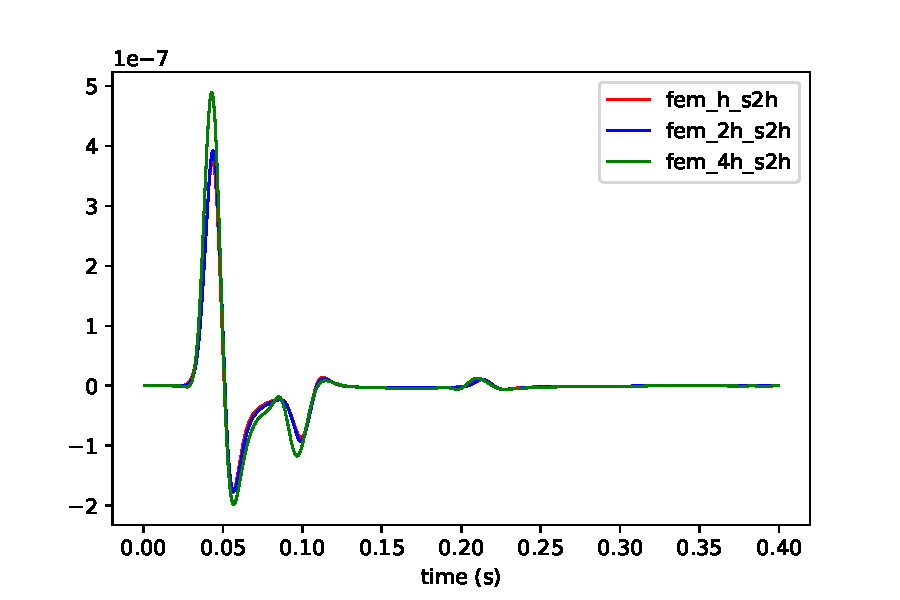
\includegraphics[width=8cm, height=5.5cm]{Thesis_Edith/figures/layered_model/layer_waves/fem_layered_tr1.pdf} 
			     \caption{}
				%\label{fig:3.7a}
		\end{subfigure}
        \hspace{0.25cm}	
		\begin{subfigure}{8cm}
				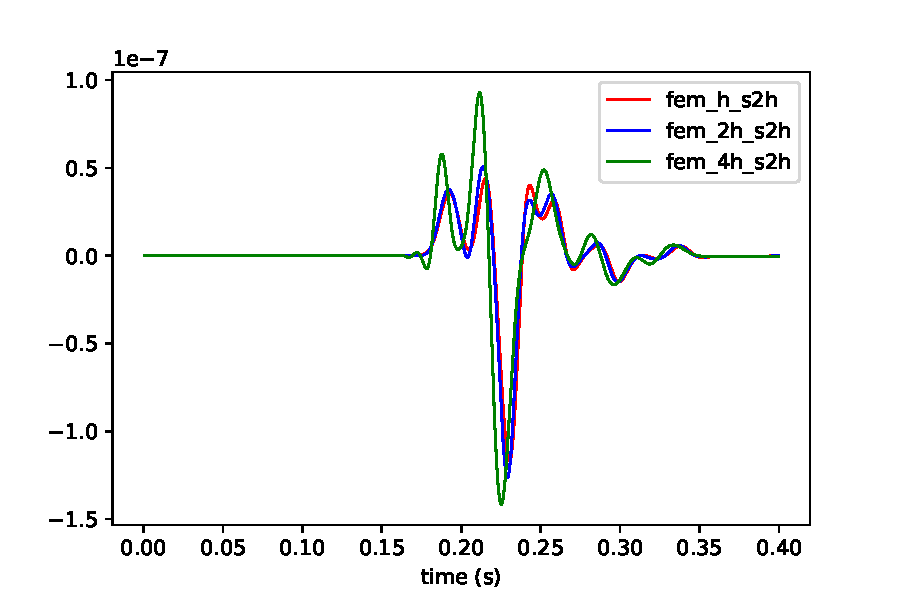
\includegraphics[width=8cm, height=5.5cm]{Thesis_Edith/figures/layered_model/layer_waves/fem_layered_tr50.pdf}
			   \caption{}
				%\label{fig:3.7b}
		\end{subfigure}
 
	\caption{Layered model: Seimograms of the reference solution and 2 additional FEM solutions in coarser meshes. (a) Seimograms from a receiver placed at 400 m in the layered model. (b) Seimograms from a receiver placed at 750 m in the layered model.}
	\label{fig:3.16}
\end{figure}

%GFEM traces
 \begin{figure}[h!]
 		\centering
		\begin{subfigure}{8cm}
				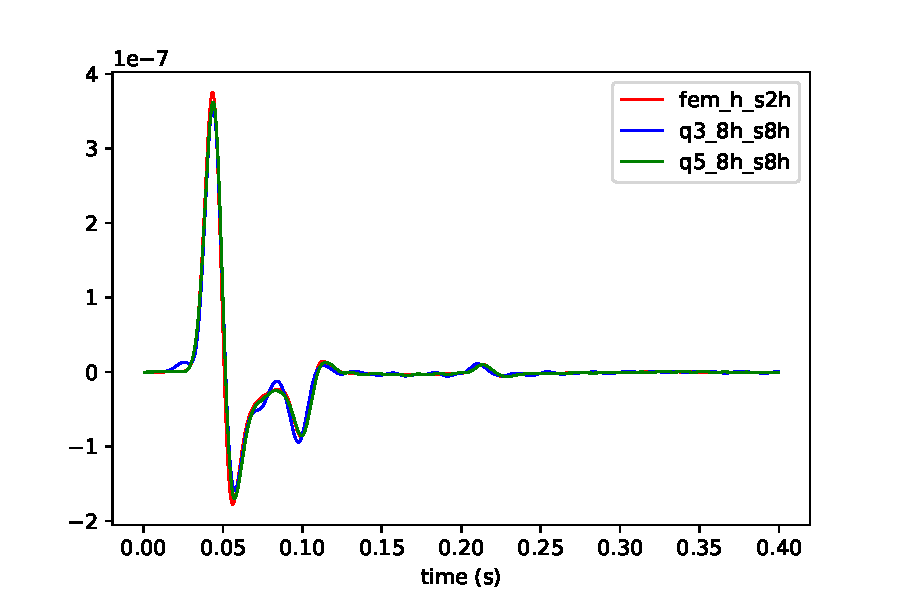
\includegraphics[width=8cm, height=5.5cm]{Thesis_Edith/figures/layered_model/layer_waves/gfem_layered_tr1.pdf} 
			     \caption{}
				%\label{fig:3.7a}
		\end{subfigure}
        \hspace{0.25cm}	
		\begin{subfigure}{8cm}
				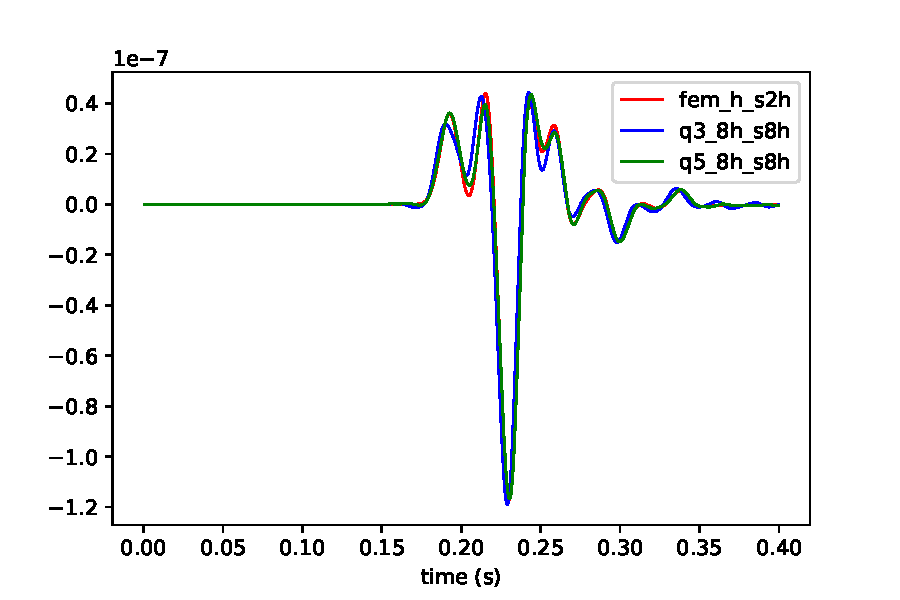
\includegraphics[width=8cm, height=5.5cm]{Thesis_Edith/figures/layered_model/layer_waves/gfem_layered_tr50.pdf}
			   \caption{}
				%\label{fig:3.7b}
		\end{subfigure}
 
	\caption{Layered model: Seismograms of the reference solution and 2 GFEM solutions with 3 and 5 plane wave directions, using a mesh and source size of $8h$. (a) Seimograms from a receiver placed at 400 m in the layered model. (b) Seimograms from a receiver placed at 750 m in the layered model.}
	\label{fig:3.17}
\end{figure}

%GFEMh traces
 \begin{figure}[h!]
 		\centering
		\begin{subfigure}{8cm}
				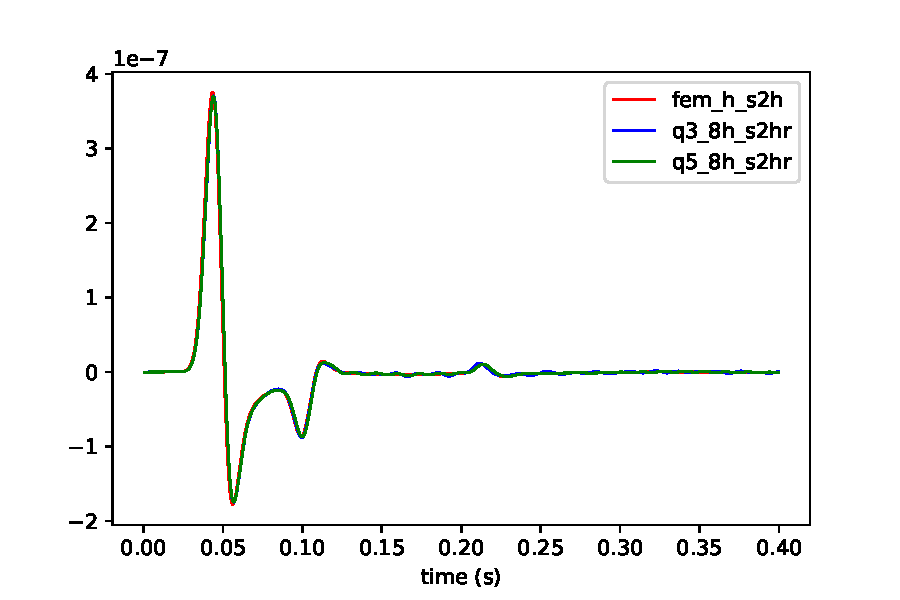
\includegraphics[width=8cm, height=5.5cm]{Thesis_Edith/figures/layered_model/layer_waves/gfemh_layered_tr1.pdf} 
			     \caption{}
				%\label{fig:3.7a}
		\end{subfigure}
        \hspace{0.25cm}	
		\begin{subfigure}{8cm}
				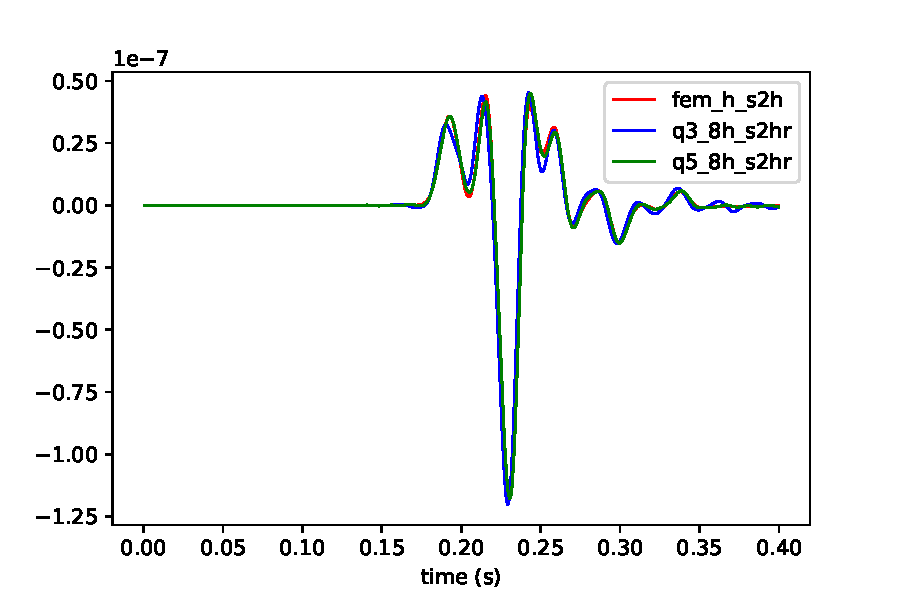
\includegraphics[width=8cm, height=5.5cm]{Thesis_Edith/figures/layered_model/layer_waves/gfemh_layered_tr50.pdf}
			   \caption{}
				%\label{fig:3.7b}
		\end{subfigure}
 
	\caption{Layered model: Seismograms of the reference solution and 2 GFEM solutions with 3 and 5 plane wave directions, using a mesh size of $8h$ and source size of $2h$. (a) Seimograms from a receiver placed at 400 m in the layered model. (b) Seimograms from a receiver placed at 750 m in the layered model.}
	\label{fig:3.18}
\end{figure}

%****
\clearpage
 Figure \ref{fig:3.19} presents the maximum cross correlation lag and two error types with respect to the reference solution for the two FEM cases calculated at the 50 receiver seismograms . Notice that the maximum cross correlation lag tend to increase as the receiver position gets further away from the source center. This effect is stronger for the FEM case with the coarsest mesh ($4h$). The errors corresponding for this FEM case are also the greatest. In general the error related to the maximum cross correlation ($E_{max}$)  is lower than the error related to the zero cross correlation $E_0$, showing the effect of mesh dispersion in the results.
 
 Figures \ref{fig:3.20} and \ref{fig:3.21} present the maximum cross correlation lag and two types of error for various GFEM cases for the 50 receiver seismograms. Figure \ref{fig:3.20} shows the effect of source size for GFEM solutions with 3 plane waves directions and Figure \ref{fig:3.21} does it for the GFEM solution with 5 plane waves directions. These results reveal that the errors decrease for  GFEM solutions when compared to the 2 FEM cases in  Figure \ref{fig:3.19} and that decreasing source radius further decreases the errors. Notice that, specially for the GFEM case with 5 plane wave directions, the lag and error are consistent across the 50 receivers, revealing less dispersive effects despite of using a very coarse mesh.
 
%Fem error
 \begin{figure}[h!]
 		\centering
		\begin{subfigure}{8cm}
				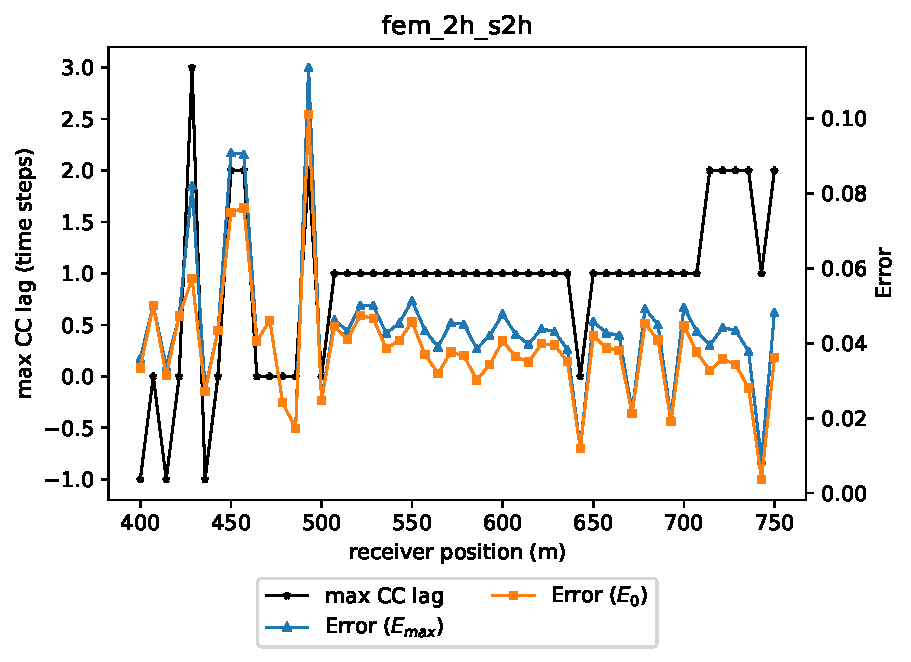
\includegraphics[width=8cm, height=5.5cm]{Thesis_Edith/figures/layered_model/layer_waves/Err_fem_2h_s2h.pdf}
			     \caption{}
				%\label{fig:3.7a}
		\end{subfigure}
        \hspace{0.25cm}	
		\begin{subfigure}{8cm}
				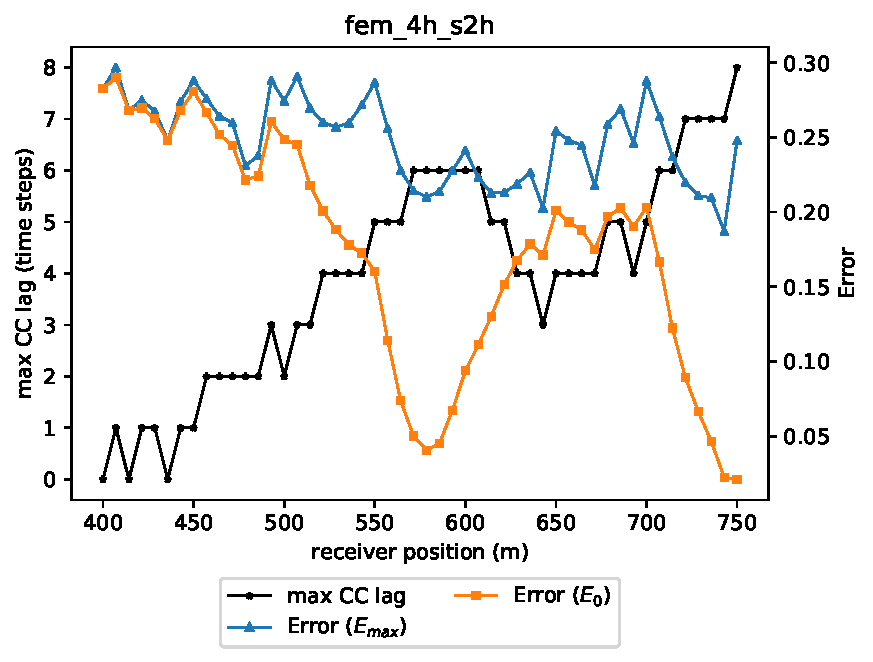
\includegraphics[width=8cm, height=5.5cm]{Thesis_Edith/figures/layered_model/layer_waves/Err_fem_4h_s2h.pdf}
			   \caption{}
				%\label{fig:3.7b}
		\end{subfigure}
 
	\caption{Layered model: Maximum cross correlation lag and errors for each receiver seismogram for 2 FEM cases. (a) For the FEM solution with mesh size of $2h$.(b) For the FEM solution with mesh size of $4h$.}
	\label{fig:3.19}
\end{figure}

%gFem error
 \begin{figure}[h!]
 		\centering
		\begin{subfigure}{8cm}
				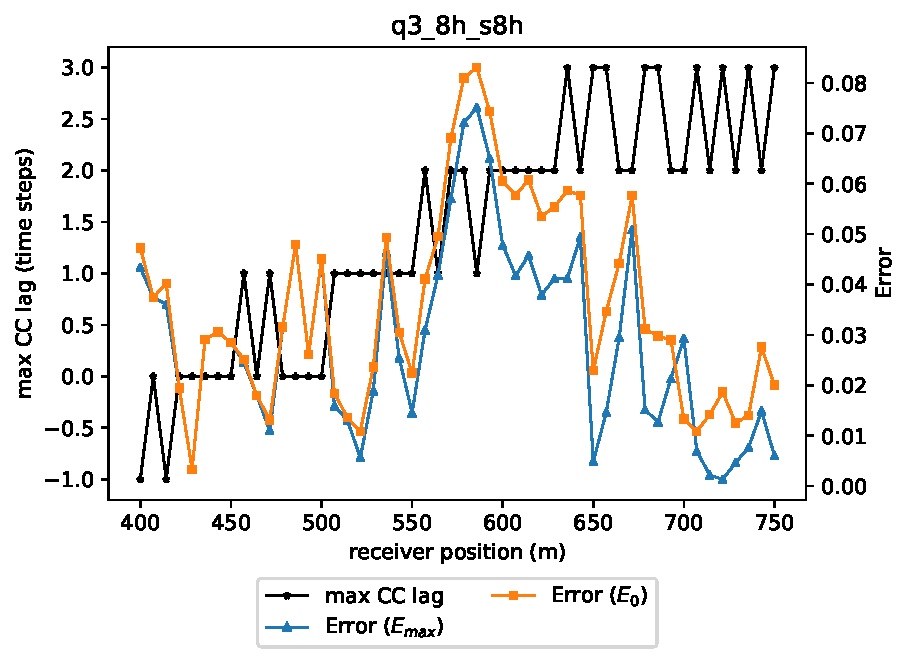
\includegraphics[width=8cm, height=6cm]{Thesis_Edith/figures/layered_model/layer_waves/Err_q3_8h_s8h.pdf}
			     \caption{}
				%\label{fig:3.7a}
		\end{subfigure}
        \hspace{0.25cm}	
		\begin{subfigure}{8cm}
				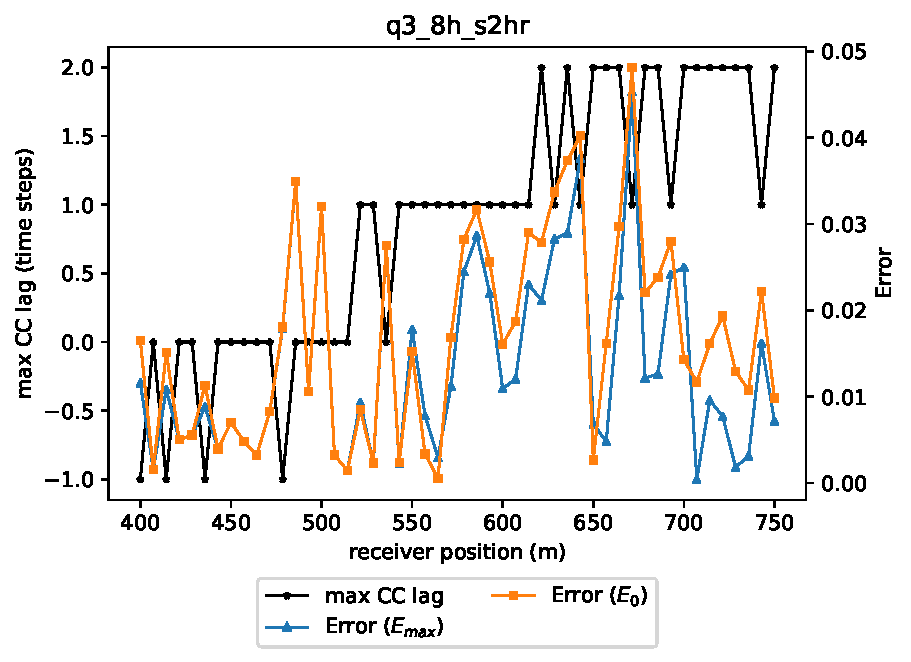
\includegraphics[width=8cm, height=6cm]{Thesis_Edith/figures/layered_model/layer_waves/Err_q3_8h_s2hr.pdf}
			   \caption{}
				%\label{fig:3.7b}
		\end{subfigure}
 
	\caption{Layered model: Maximum cross correlation lag and errors for each receiver seismogram for 2 GFEM solutions with 3 plane wave directions and mesh size of $8h$. (a) For the GFEM solution with source size of $8h$. (b) For the GFEM solution with source size of $2h$}
	\label{fig:3.20}
\end{figure}

%gFem error
 \begin{figure}[h!]
 		\centering
		\begin{subfigure}{8cm}
				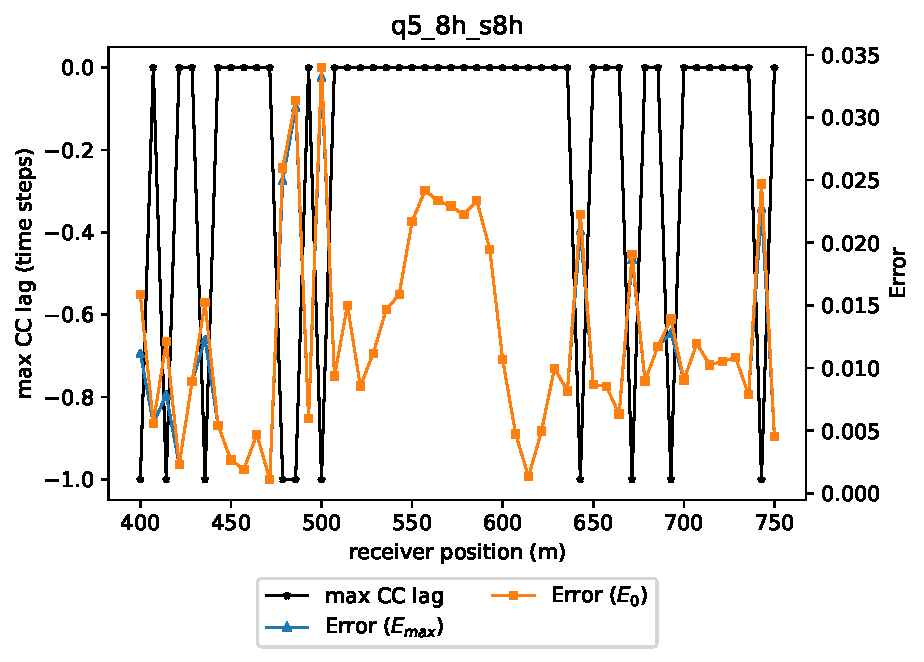
\includegraphics[width=8cm, height=6cm]{Thesis_Edith/figures/layered_model/layer_waves/Err_q5_8h_s8h.pdf}
			     \caption{}
				%\label{fig:3.7a}
		\end{subfigure}
        \hspace{0.25cm}	
		\begin{subfigure}{8cm}
				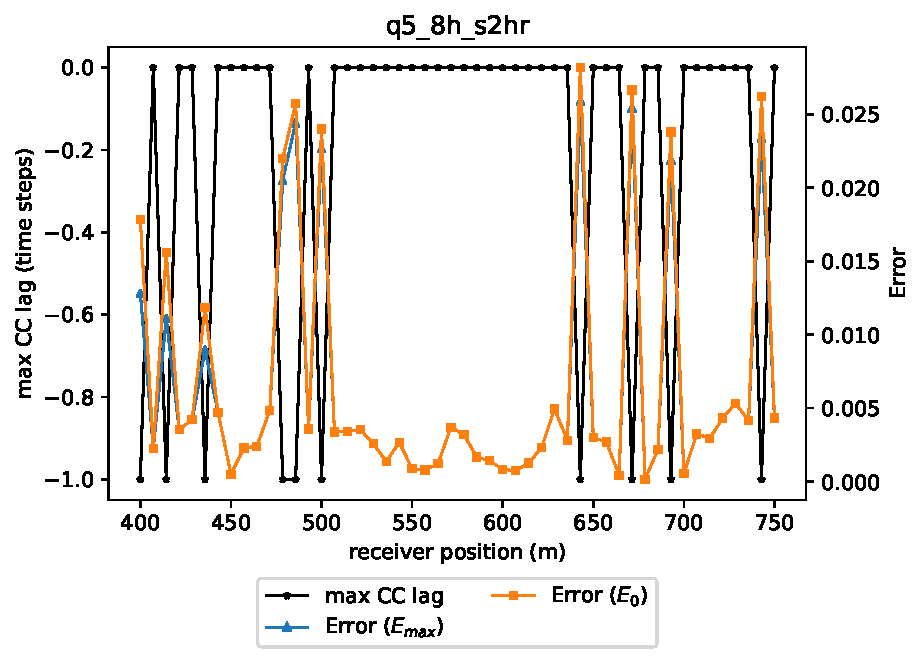
\includegraphics[width=8cm, height=6cm]{Thesis_Edith/figures/layered_model/layer_waves/Err_q5_8h_s2hr.pdf}
			   \caption{}
				%\label{fig:3.7b}
		\end{subfigure}
 
	\caption{Layered model: Maximum cross correlation lag and errors for each receiver seismogram for 2 GFEM solutions with 5 plane wave directions and mesh size of $8h$. (a) For the GFEM solution with source size of $8h$. (b) For the GFEM solution with source size of $2h$}
	\label{fig:3.21}
\end{figure}

Figure \ref{fig:3.22} shows the mean error versus relative simulation time and standard deviation for the FEM solutions and for various GFEM cases. According to theses results, the GFEM cases are faster than the FEM reference solution and than the FEM solution in a mesh of $2h$ inclusive. The fastest solutions belong to the GFEM solutions implemented with 3 plane waves directions, due to their lower number of DOFs.
Regarding the mean error, all but one GFEM solution present lower error than any of the FEM solutions is coarser meshes of $2h$ and $4h$, and the GFEM solutions with 5 plane waves directions presents the 2 lowest errors. 
For the standard deviation, results trends resemble those of the mean error vs time, with lower standard deviation corresponding to the GFEM cases except one and with the 2 lowest standard deviation corresponding to the GFEM solutions with 5 plane wave directions. Observe as well that the accuracy of GFEM results improve with the smallest source size. 


% Time v error
%*******
 \begin{figure}[h!]
 		\centering
		\begin{subfigure}{8cm}
				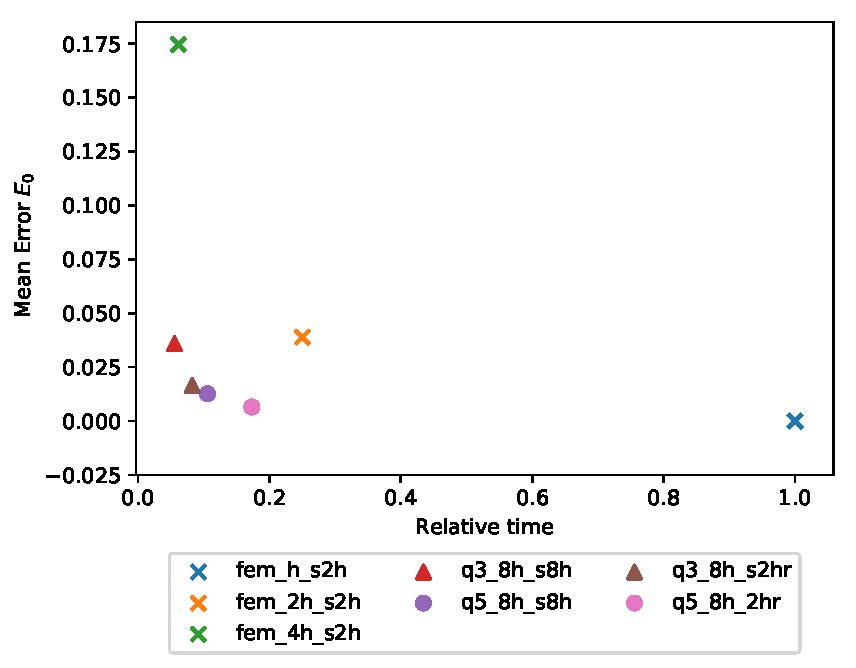
\includegraphics[width=8cm, height=6cm]{Thesis_Edith/figures/layered_model/layer_waves/MeanError_time_layered.pdf}
			     \caption{}
				%\label{fig:3.7a}
		\end{subfigure}
        \hspace{0.25cm}	
		\begin{subfigure}{8cm}
				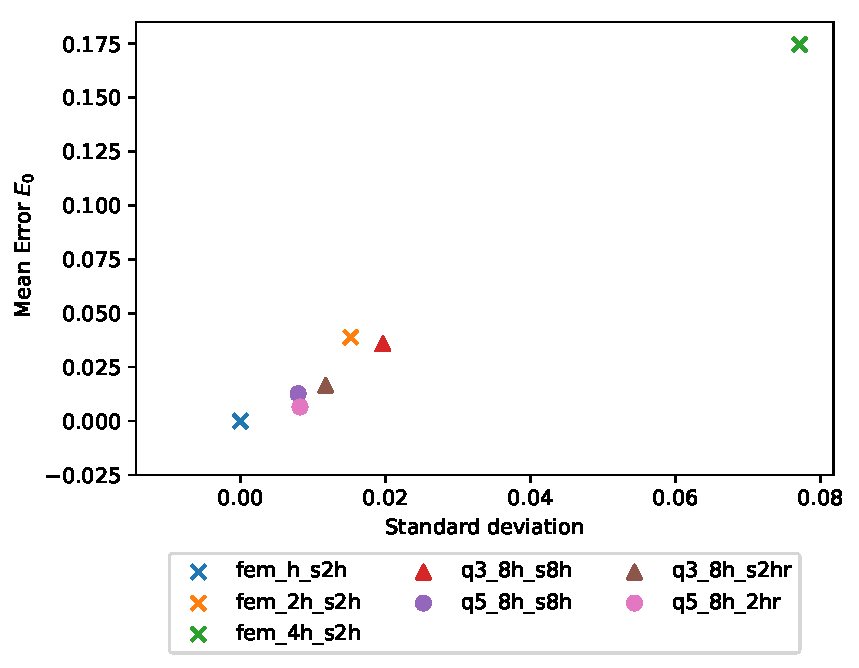
\includegraphics[width=8cm, height=6cm]{Thesis_Edith/figures/layered_model/layer_waves/MeanError_std_layered.pdf}
			   \caption{}
				%\label{fig:3.7b}
		\end{subfigure}
 
	\caption{Layered model: Mean error vs relative time and standard deviation for various FEM and GFEM cases. (a) Mean error vs relative time. (b) Mean error vs standard deviation.}
	\label{fig:3.22}
\end{figure}


 \clearpage
% New section: Scattering Model
%*******************************
\section{Case 3: Model with Karst Inclusion (Scattering Model)}
The model for this example is as shown in Figure \ref{fig:3.23}. This model is similar to the layered model, however for this case the top layer velocity is half of that in the layered model, to simulate a poor consolidated layer. This model also presents a karst inclusion which is assumed to be full of water. The main goal of this simulation model is to show the capability of the GFEM approach to combine flexible local refinement with its computational efficiency. 

 In this model, The source is located at the same position as in the layered model: -50 m in the vertical coordinate and 400 m in the horizontal coordinate and has a frequency of 40 Hz. There are 100 receivers placed close to the surface and span from 50 m to 750 m in the horizontal coordinates. Table \ref{table:3.2} shows the velocity, wavelengths and wavenumbers for each of the geological features present in the model. It also shows the number cells per wavelength for different mesh sizes.

 \begin{figure}[h!]
	\centering
	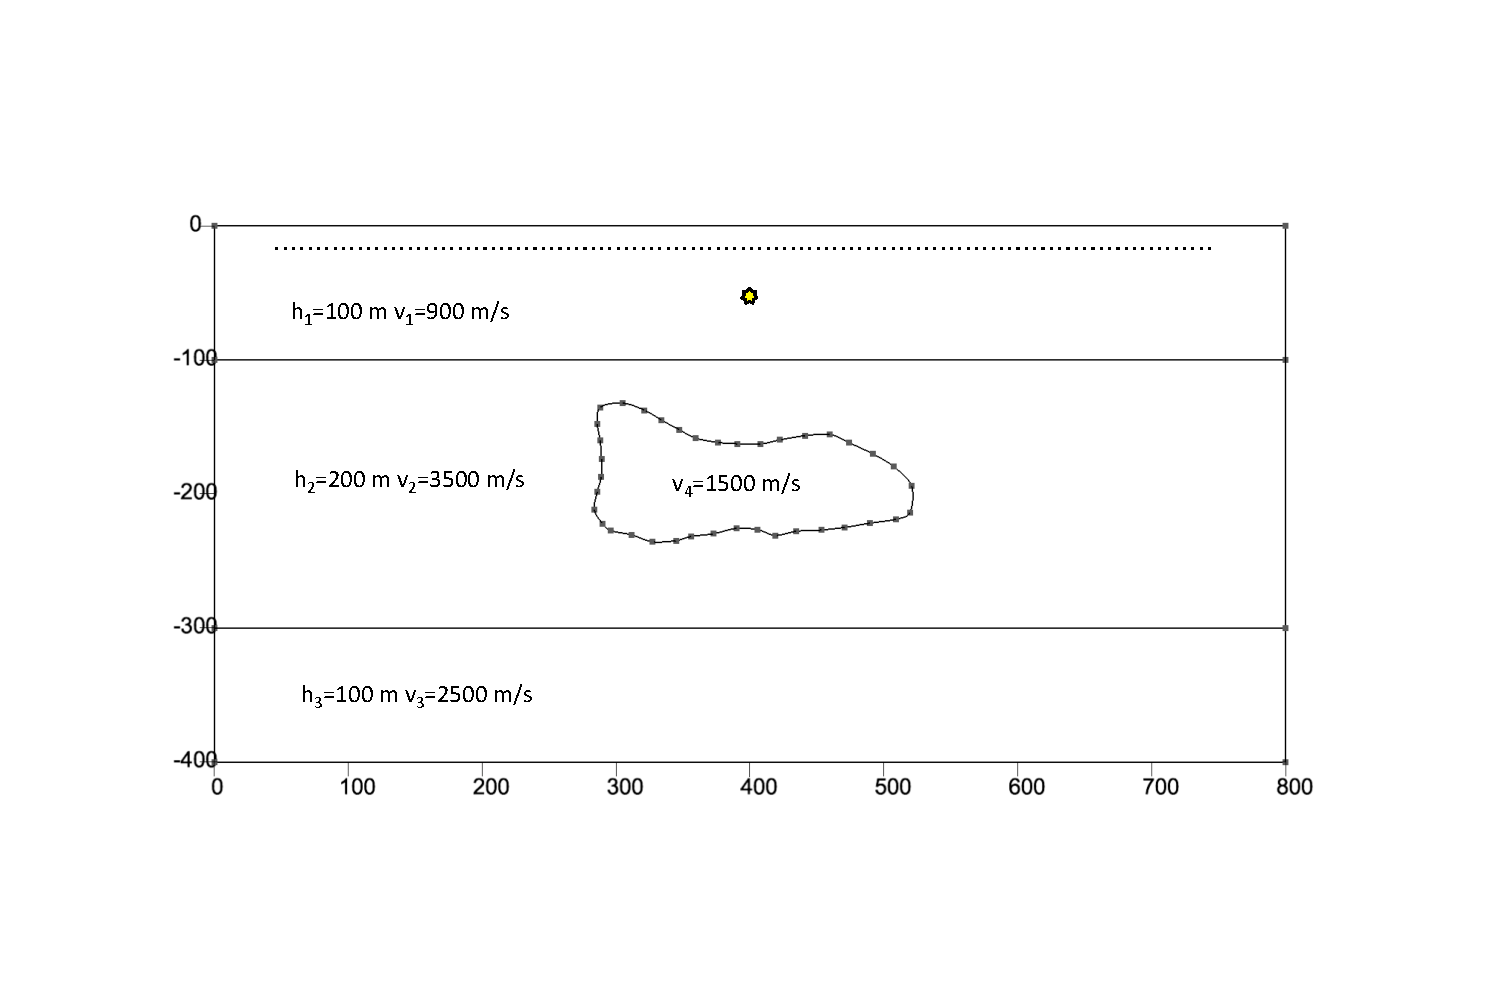
\includegraphics[width=14cm, height=7cm]{Thesis_Edith/figures/scattering/scatter_source.pdf}
	\caption{Scattering model with a seismic source in the first layer (yellow star) and a horizontal array of 100 receivers close to surface as depicted by the dotted line.}
	\label{fig:3.23}
\end{figure}

%table
\begin{table}[h!]
\footnotesize
\centering
    \begin{tabular}{|c|m{1.5cm}|m{2cm}|m{2cm}|m{1cm}| m{0.8cm}|m{0.8cm}|m{0.8cm}|m{0.8cm}|}
      \hline
      \multirow{2}{*}{Feature} &
      \multirow{2}{1.5cm}{Velocity (m/s)} &
      \multirow{2}{2cm}{Wavelength \quad $\lambda$ (m)} &
      \multirow{2}{2cm}{Wavenumber  k (m$^{-1}$)} &
         \multicolumn{5}{m{5cm}|}{Number of cells per wavelength in a mesh size of :} \\
         & & &  &$h/2$ & $h$ & $2h$ & $4h$ & $8h$ \\
      \hline
      1 & 900 & 22.5 & 0.28 & 28.8 & 14.4 & 7.2 & 3.6 & 1.8\\
      \hline
      2 & 3500 & 87.5 & 0.07 & 112 & 56 & 28 & 14 & 7\\
      \hline
      3 & 2500 & 62.5 & 0.10 & 80 & 40 & 20 & 10 & 5\\
      \hline
      4 & 1500 & 37.5 & 0.17 & 48 & 24 & 12 & 6 & 3\\
       \hline
    \end{tabular}
    \caption{Scattering model: Table showing the velocity, wavelength and wavenumber for each geological feature in the model, as well as the number cells per wavelength in different mesh sizes. Source frequency is 40 Hz and $h=$1.5625 m}
    \label{table:3.2}
\end{table}

For the reference solution, I use a similar mesh as in Figure \ref{fig:3.24}, but for this case the mesh size is $h$ except for the top layer, for which a mesh size of $h/2$ is used. I use similar coarser meshes - of sizes $2h$ and $4h$ and top layer mesh sizes of $h$ and $2h$ correspondingly -  to run two additional FEM cases. 
For the GFEM simulation cases I use two mesh configurations: one as shown in Figure \ref{fig:3.25}, with a background mesh size of $8h$ and of size $4h$ for the top layer. The second mesh  is as in Figure \ref{fig:3.26}, which is similar to the first one but with additional refinement around the karst feature. The goal of this additional refinement is to conform better to the karst geometrical shape, and as consequence obtain a more accurate simulation. For all the GFEM cases the wave number used for the plane wave enrichments is 0.28 m$^{-1}$, calculated by dividing the source radial frequency by the lowest geological feature velocity (900 m/s).

%Meshes
 \begin{figure}[h!]
	\centering
	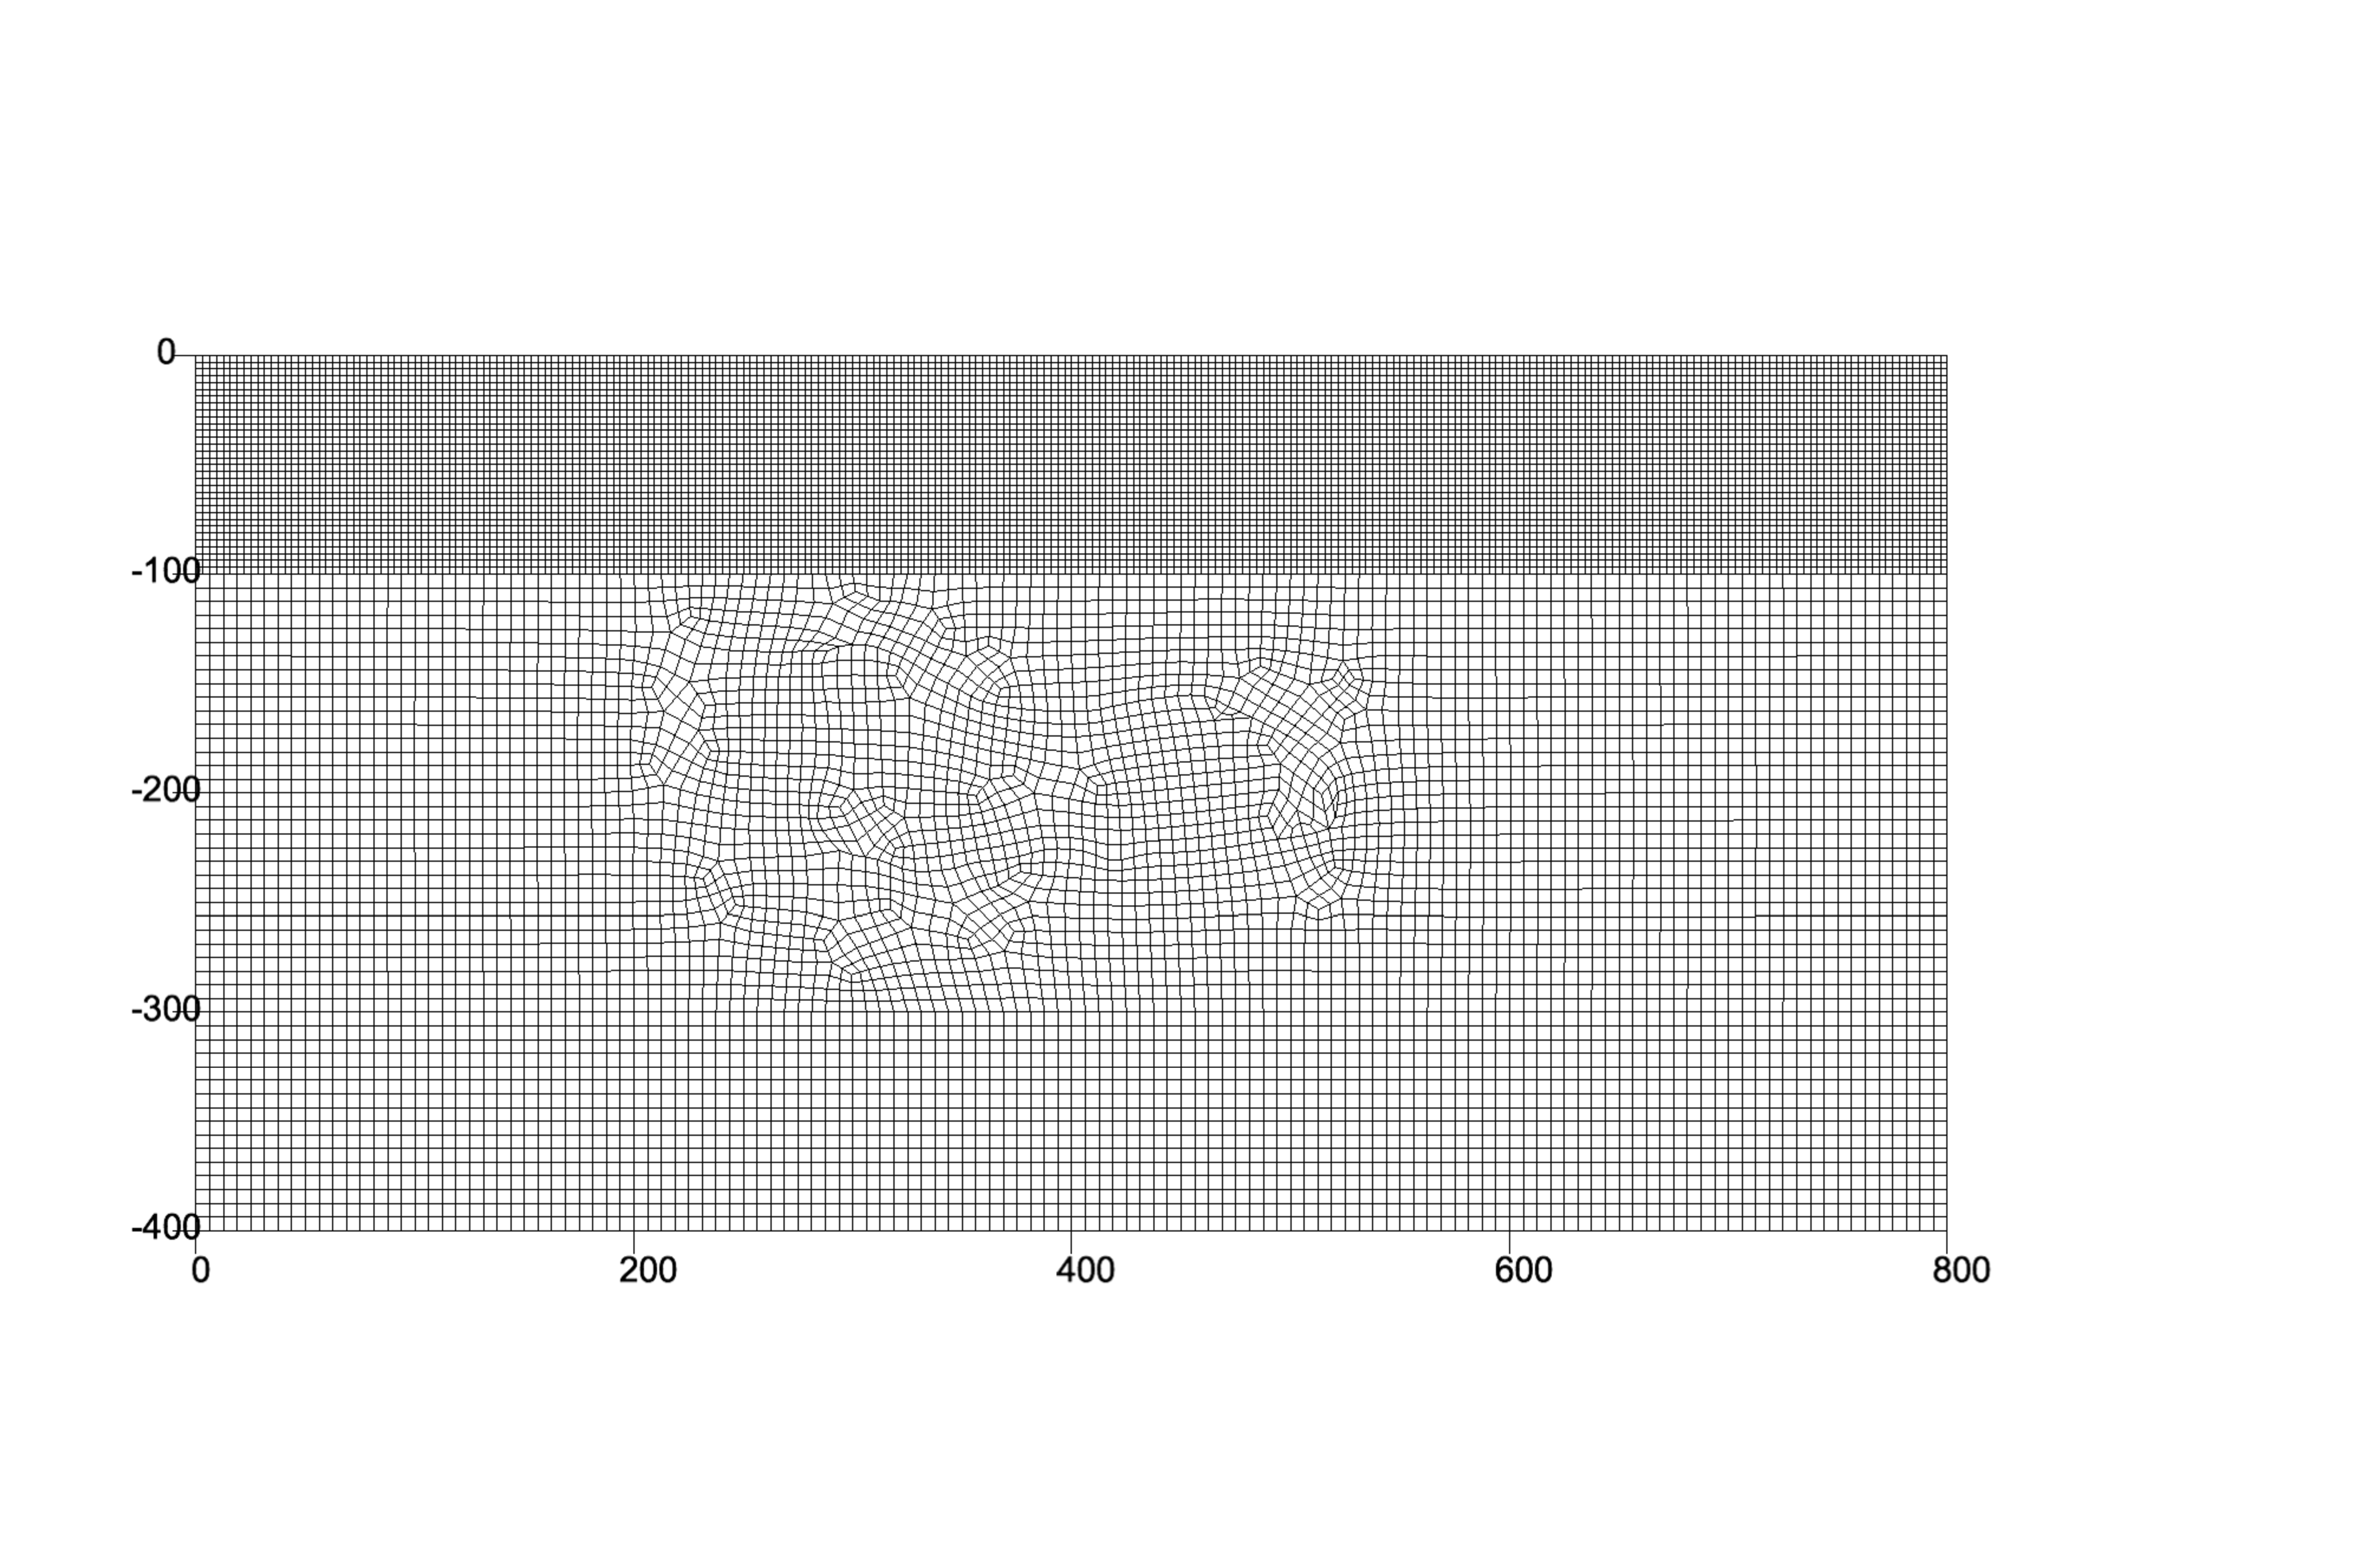
\includegraphics[width=16cm, height=8cm]{Thesis_Edith/figures/scattering/mesh_ref_mr4_v2.pdf}
	\caption{Scattering model: Example of one of the meshes used for the  standard FEM simulations. The original mesh with grid size of $4h$ is subdivided in half ($2h$) at the top layer.}
	\label{fig:3.24}
\end{figure}

 \begin{figure}[h!]
	\centering
	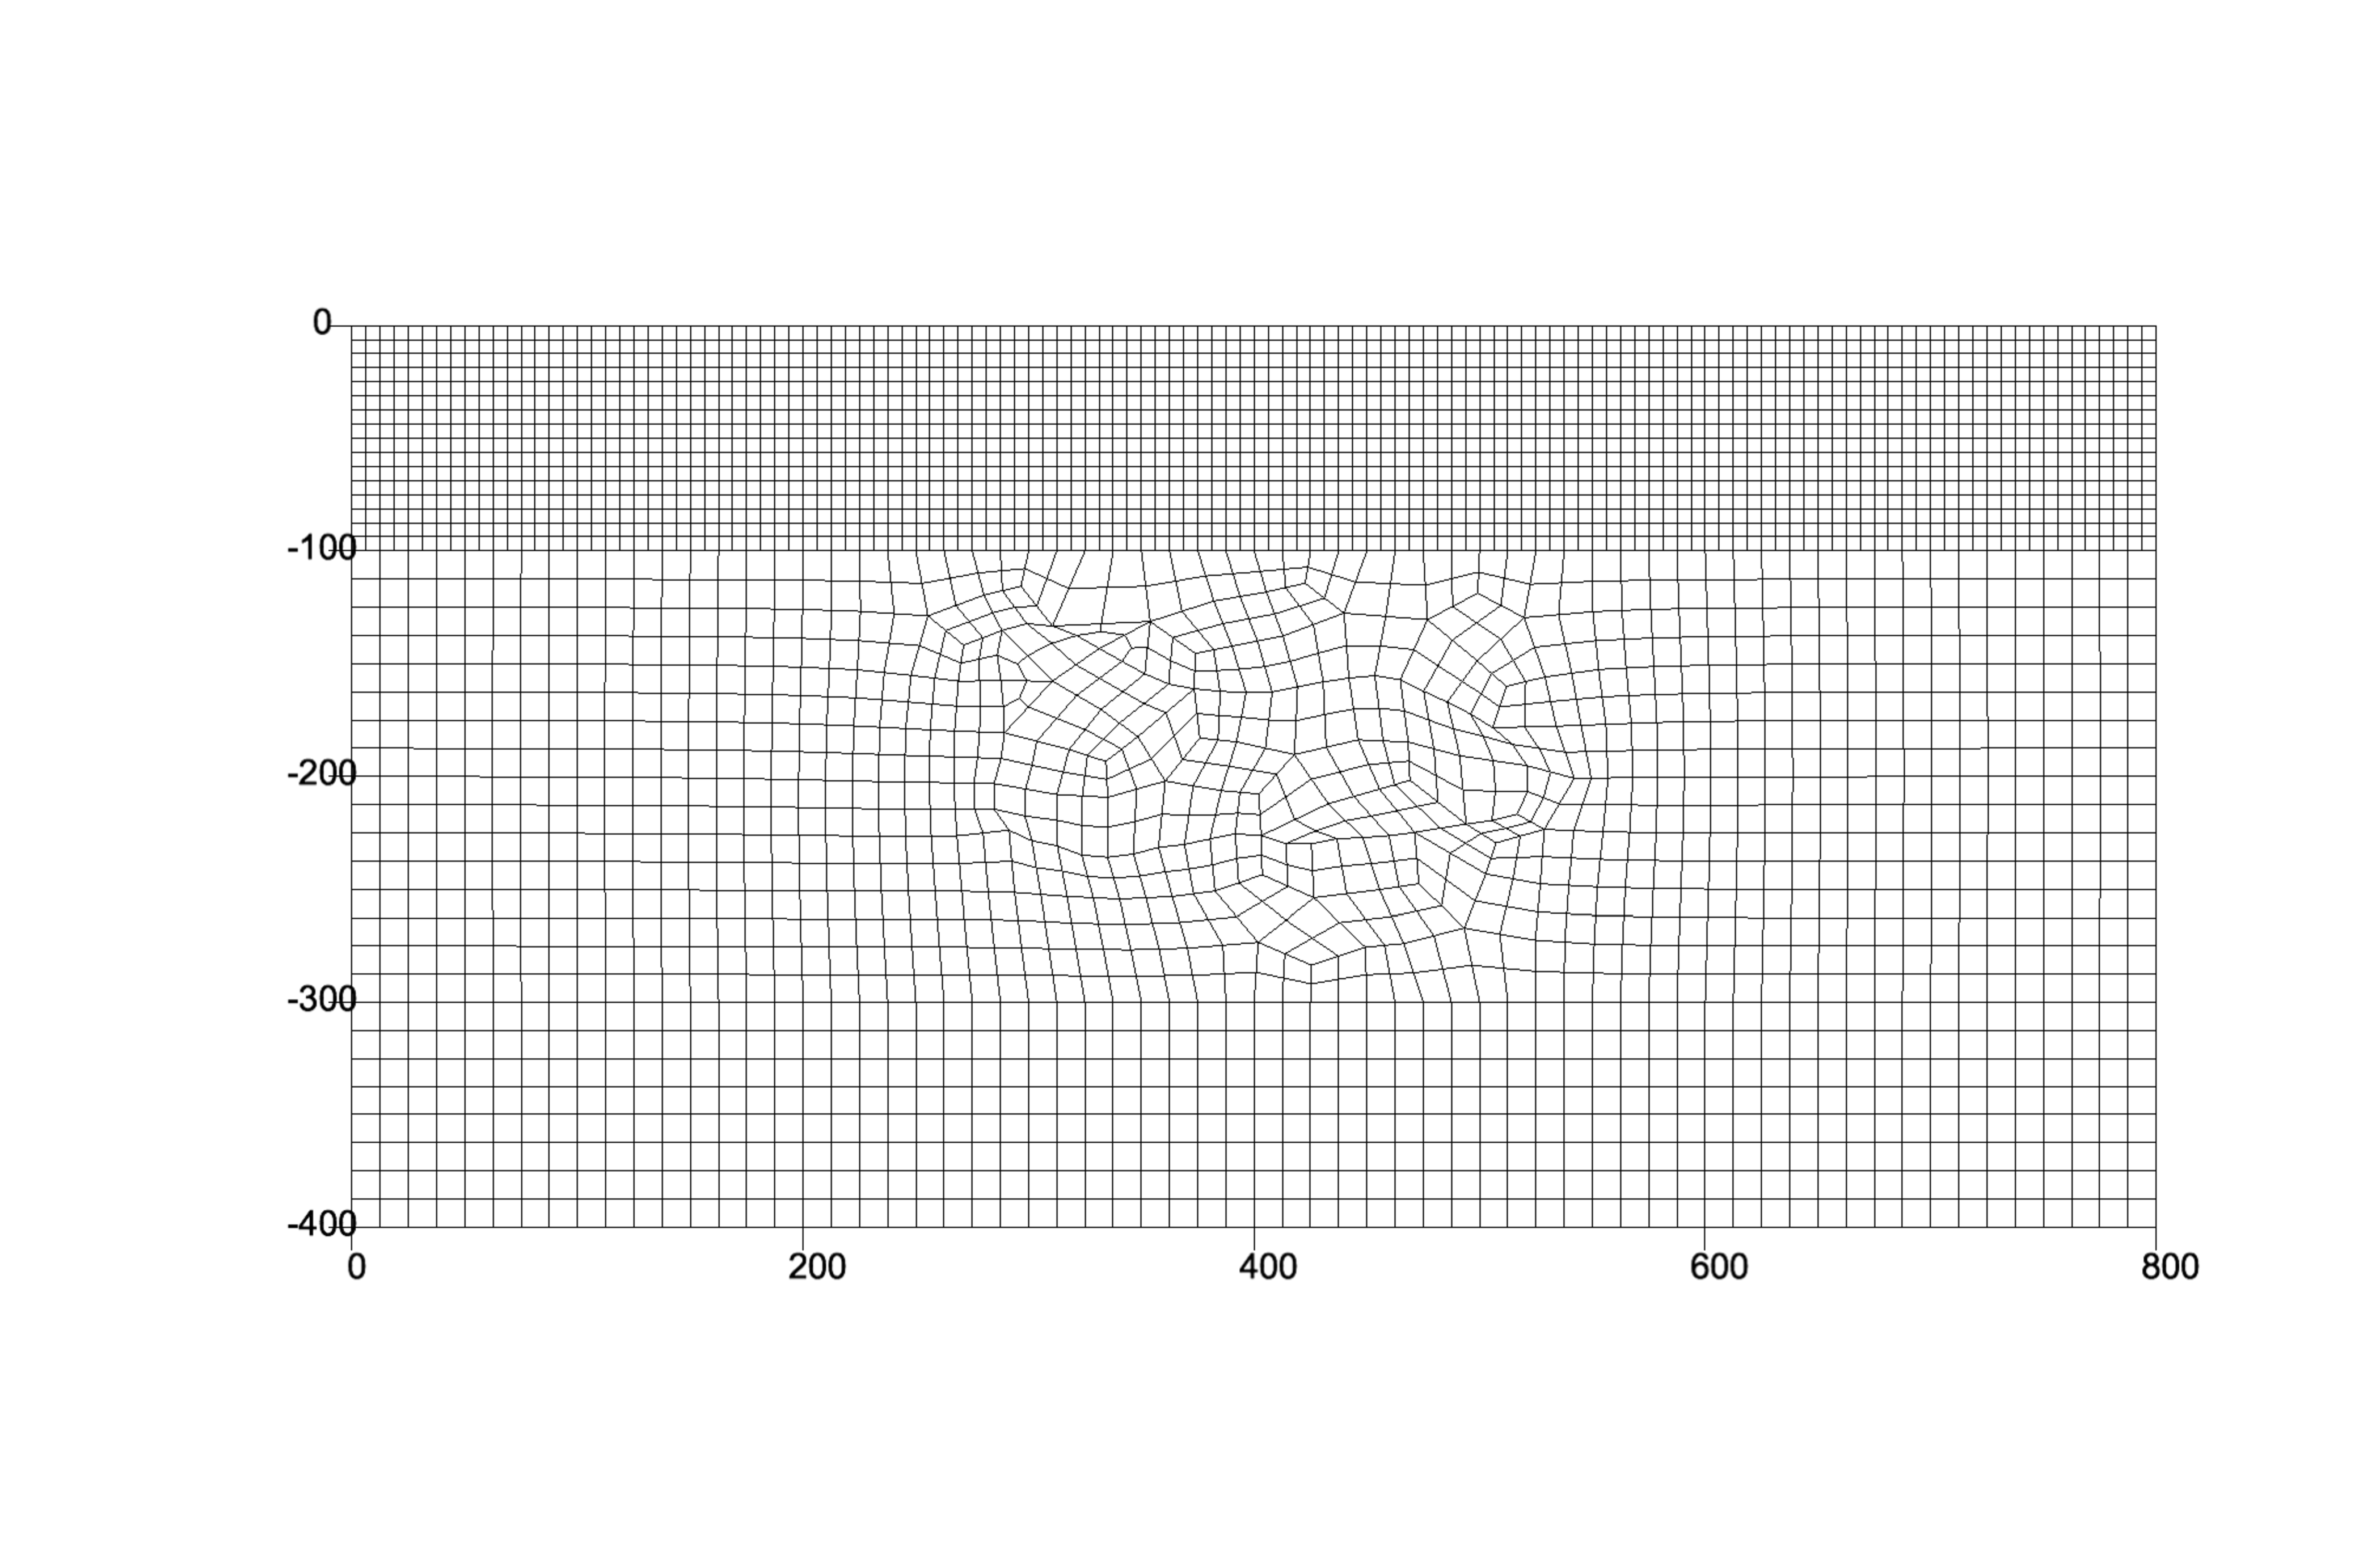
\includegraphics[width=16cm, height=8cm]{Thesis_Edith/figures/scattering/mesh_ref_mr3_v2.pdf}
	\caption{Scattering model: Example of a type of mesh used for the GFEM simulations. The original mesh with grid size of $8h$ is subdivided in half ($4h$) at the top layer.}
	\label{fig:3.25}
\end{figure}

 \begin{figure}[h!]
	\centering
	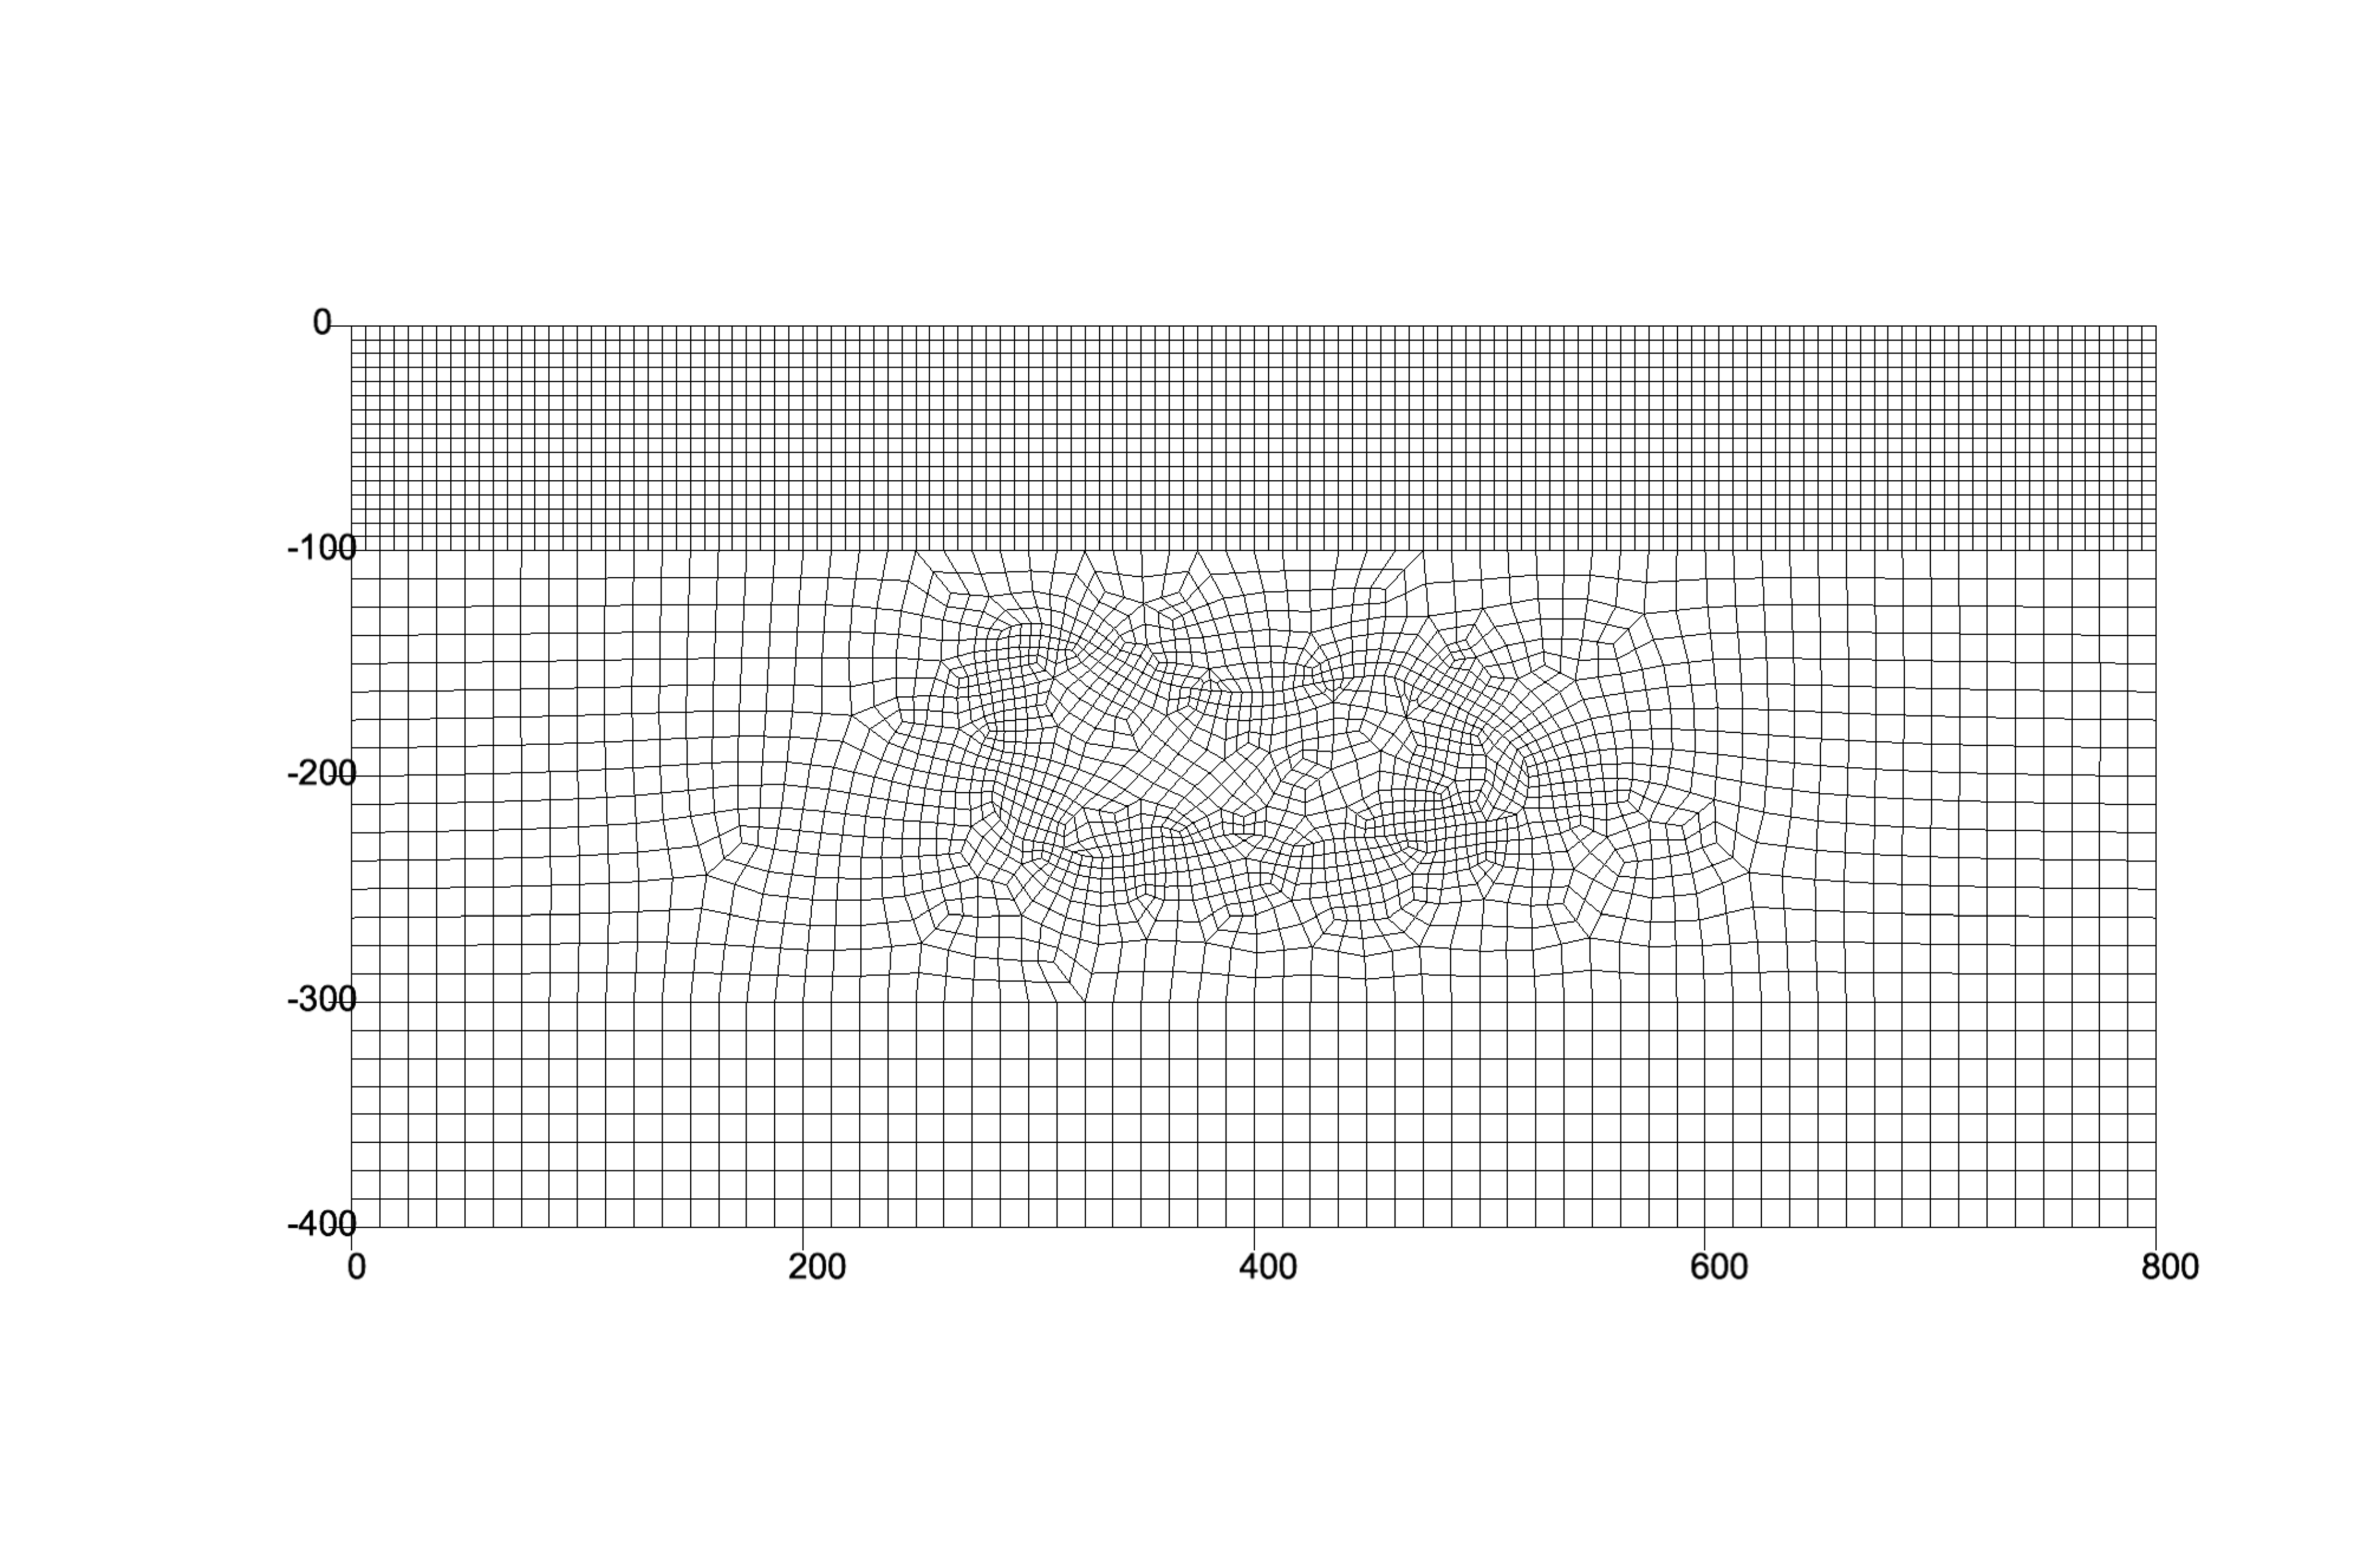
\includegraphics[width=16cm, height=8cm]{Thesis_Edith/figures/scattering/meshr_ref_v2.pdf}
	\caption{Scattering model: Example of a type of mesh used for GFEM simulations. This mesh is similar to the mesh in Figure \ref{fig:3.25} with additional refinement around the karst inclusion.}
	\label{fig:3.26}
\end{figure}

%******
\clearpage
Figure \ref{fig:3.27} shows the seismogram of the shot gather for the reference solution. Prominent features are the direct wave, the reflection at the bottom of the top layer and the multiple scattering effects produced by the karst inclusion.
%shot gather
 \begin{figure}[h!]
	\centering
	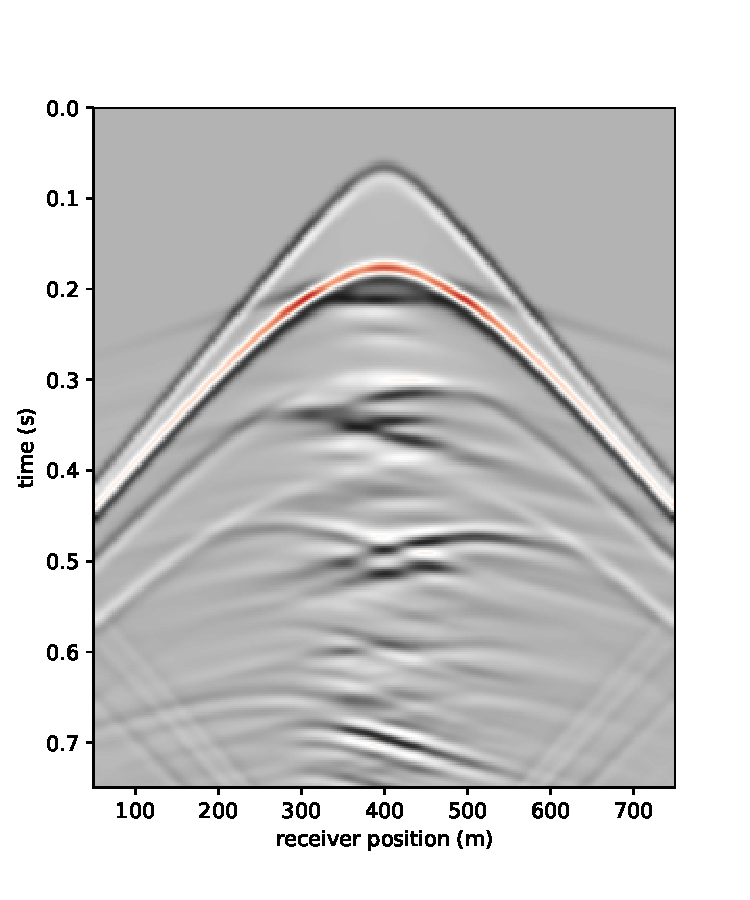
\includegraphics[width=10cm, height=13cm]{Thesis_Edith/figures/scattering/scat_waves/seismogram_scattering.pdf}
	\caption{Scattering model: Seismograms of the shot gather for the reference solution. Divergence coefficient is 2.5}
	\label{fig:3.27}
\end{figure}

%******
\clearpage
Figure \ref{fig:3.28} shows the seismograms for the reference solution and 2 additional FEM simulation cases with coarser meshes for receivers placed at 156.1 m and 580.3 m in the horizontal coordinate. As expected simulation results deteriorate in accuracy as the mesh is coarsened when compared to the reference solution.

Figures \ref{fig:3.29} and \ref{fig:3.30} show the seismograms for the reference solution and GFEM simulation cases with 5 plane wave directions obtained for receivers placed at 156.1 m and 580.3 m in the horizontal coordinate respectively. In both of these figures I compare the effect of source size and of the additional refinement around the karst feature. As found in the layered model example, a decrease in source size improves the accuray of the simulation result. The additional refinement around the karst feature also improves the match of reflections coming at later times with the reference solution as pointed by the arrows in the figures.

Figure \ref{fig:3.31} shows the seismograms for the reference solution and for a GFEM simulation case with 3 plane wave directions obtained for receivers placed at 156.1 m and 580.3 m in the horizontal coordinate respectively. I this case I use a mesh as in figure \ref{fig:3.24} with no additional refinement around the karst inclusion. This is the same mesh used for the FEM case with the coarsest mesh. However, when compared the results of GFEM  with that of the corresponding FEM in figure  \ref{fig:3.28}, the GFEM outcomes are much more accurate.


%fem traces
 \begin{figure}[h!]
 		\centering
		\begin{subfigure}{8cm}
				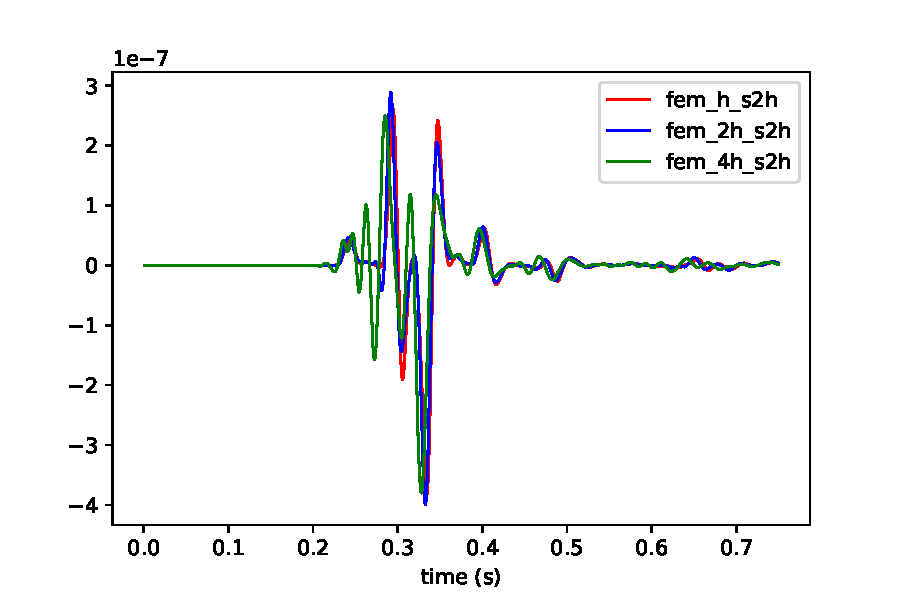
\includegraphics[width=8cm, height=5.5cm]{Thesis_Edith/figures/scattering/scat_waves/fem_scat_tr15.pdf} 
			     \caption{}
				%\label{fig:3.7a}
		\end{subfigure}
        \hspace{0.25cm}	
		\begin{subfigure}{8cm}
				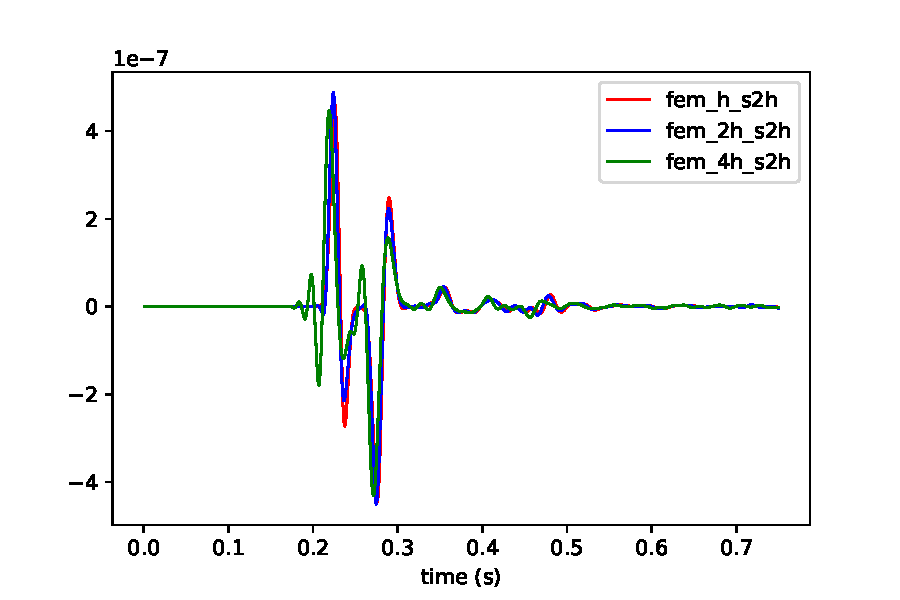
\includegraphics[width=8cm, height=5.5cm]{Thesis_Edith/figures/scattering/scat_waves/fem_scat_tr75.pdf}
			   \caption{}
				%\label{fig:3.7b}
		\end{subfigure}
 
	\caption{Scattering model: Seismograms of the reference solution in a mesh size of $h$ and $h/2$ at the top layer and for 2 additional FEM solutions in coarser meshes. (a) Seimograms from a receiver located at 156.1 m in the horizontal coordinate. (b) Seimograms from a receiver located at 580.3 m in the horizontal coordinate.}
	\label{fig:3.28}
\end{figure}

%gfem traces
 \begin{figure}[h!]
 		\centering
		\begin{subfigure}{8cm}
				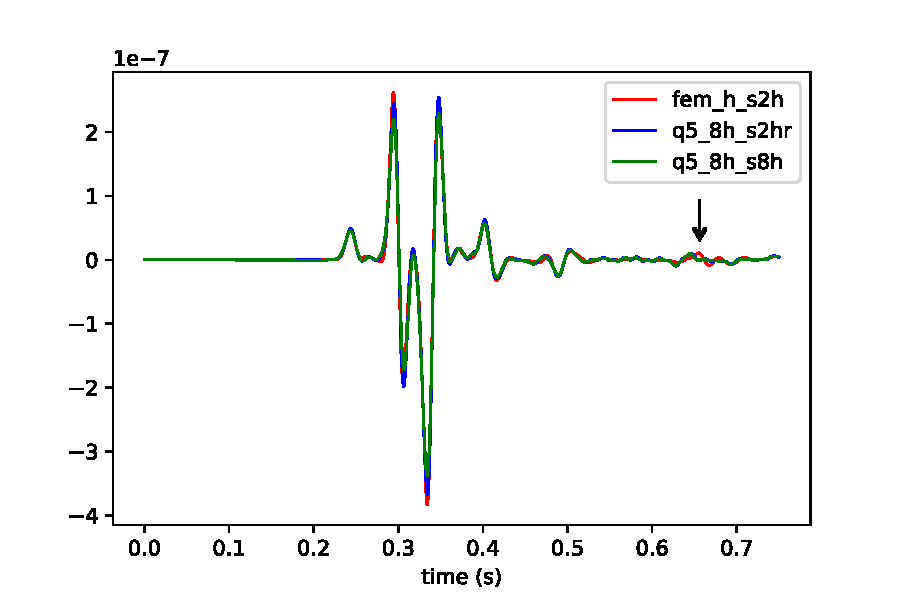
\includegraphics[width=8cm, height=5.5cm]{Thesis_Edith/figures/scattering/scat_waves/gfem_scat_tr15_v2.pdf} 
			     \caption{}
				%\label{fig:3.7a}
		\end{subfigure}
        \hspace{0.25cm}	
		\begin{subfigure}{8cm}
				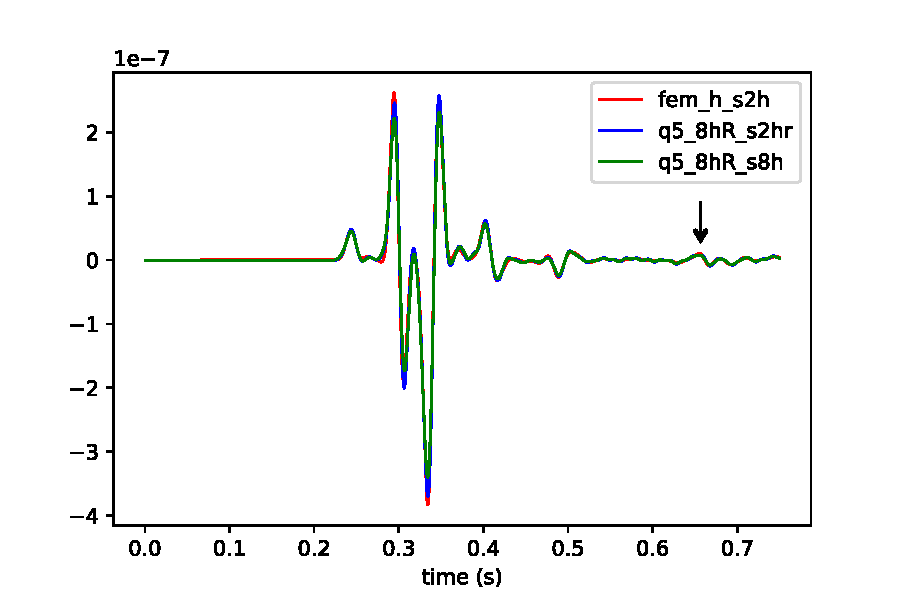
\includegraphics[width=8cm, height=5.5cm]{Thesis_Edith/figures/scattering/scat_waves/gfemr_scat_tr15_v2.pdf}
			   \caption{}
				%\label{fig:3.7b}
		\end{subfigure}
 
	\caption{Scattering model: Seismograms from a receiver located at 156.1 m in the horizontal coordinate for the reference solution and  GFEM solutions obtained   with 5 plane wave directions and with  a source radius of $2h$ and $8h$. (a) Seismograms showing GFEM solutions obtained in a mesh as in Figure \ref{fig:3.25}. (b) Seismograms showing GFEM solutions obtained in a mesh as in Figure \ref{fig:3.26}. Arrows show the difference in the GFEM seismograms.}
	\label{fig:3.29}
\end{figure}

 \begin{figure}[h!]
 		\centering
		\begin{subfigure}{8cm}
				\includegraphics[width=8cm, height=5.5cm]{Thesis_Edith/figures/scattering/scat_waves/gfem_scat_tr75_v2.pdf} 
			     \caption{}
				%\label{fig:3.7a}
		\end{subfigure}
        \hspace{0.25cm}	
		\begin{subfigure}{8cm}
				\includegraphics[width=8cm, height=5.5cm]{Thesis_Edith/figures/scattering/scat_waves/gfemr_scat_tr75_v2.pdf}
			   \caption{}
				%\label{fig:3.7b}
		\end{subfigure}
 
	\caption{Scattering model: Seismograms from a receiver located at 580.3 m in the horizontal coordinate for the reference solution and  GFEM solutions obtained  with  with 5 plane wave directions and a source radius of $2h$ and $8h$. (a) Seismograms showing GFEM solutions obtained in a mesh as in Figure \ref{fig:3.25}. (b) Seismograms showing GFEM solutions obtained in a mesh as in Figure \ref{fig:3.26}. Arrows show the difference between the GFEM seismograms in (a) and (b).}
	\label{fig:3.30}
\end{figure}

 \begin{figure}[h!]
 		\centering
		\begin{subfigure}{8cm}
				\includegraphics[width=8cm, height=5.5cm]{Thesis_Edith/figures/scattering/scat_waves/gfem3_scat_tr15.pdf}
			     \caption{}
				%\label{fig:3.7a}
		\end{subfigure}
        \hspace{0.25cm}	
		\begin{subfigure}{8cm}
				\includegraphics[width=8cm, height=5.5cm]{Thesis_Edith/figures/scattering/scat_waves/gfem3_scat_tr75.pdf}
			   \caption{}
				%\label{fig:3.7b}
		\end{subfigure}
 
	\caption{Scattering model: Scattering model: Seismograms from a receiver located at 580.3 m in the horizontal coordinate for the reference solution and a GFEM solution obtained with 3 plane wave directions, in a mesh of size  $4h$ and $2h$ at the top layer and with a source radius of $2h$.}
	\label{fig:3.31}
\end{figure}

\clearpage
 Figure \ref{fig:3.32} presents the maximum cross correlation lag and two error types with respect to the reference solution, calculated for the two FEM simulations across the 100 receiver seismograms. As noted in the layered model error analysis, the maximum cross correlation lag and the associated errors increase as the receivers get further away from the source center (400 m). This effect is the greatest for the FEM with the coarsest mesh. As also noted before, the error related to the maximum cross correlation ($E_{max}$) is lower than the one related to the zero lag cross correlation ($E_0$) and their difference increases as the source-receiver offset increases. These results show not only the numerical error as the seismic wave travels further away from the source but also the dispersion error caused by increasing the mesh size.
 
 Figures \ref{fig:3.33} and \ref{fig:3.34} show the maximum cross correlation lag and two error types with respect to the reference solution for several GFEM cases obtained with 5 plane wave directions. Each of these figures compare the effect of refinement around the karst inclusion as source size is kept constant. Note that in both figures, there are results spiking up from the average.  These spikes correspond to receivers located at 467.2 m and 474.2 m. I examine possible causes of these anomalous outputs in the appendix. Disregarding the two irregular outputs in all figures, the effect of the additional refinement around the karstic feature is practically imperceptible, however the effect of decreasing source size is evident, causing a decrease in the errors. Overall, as mentioned for the layered model, errors are consistent across the 100 receivers, showing little dispersion effect. 
 Figure \ref{fig:3.35} shows the maximum cross correlation lag and two error types with respect to the reference solution for an additional GFEM case obtained with 3 plane wave directions. For this case, a minimum error lag of -1 time step exist for the receivers at both ends and in general the errors are consistent in average across the 100 receivers, increasing slightly as the receivers get further away from the center of the source. 
 
%fem error
 \begin{figure}[h!]
 		\centering
		\begin{subfigure}{8cm}
				\includegraphics[width=8cm, height=5.5cm]{Thesis_Edith/figures/scattering/scat_waves/Err_fem_2h.pdf}
			     \caption{}
				%\label{fig:3.7a}
		\end{subfigure}
        \hspace{0.25cm}	
		\begin{subfigure}{8cm}
				\includegraphics[width=8cm, height=5.5cm]{Thesis_Edith/figures/scattering/scat_waves/Err_fem_4h.pdf}
			   \caption{}
				%\label{fig:3.7b}
		\end{subfigure}
 
	\caption{Scattering model: Maximum cross correlation lag and errors for 100 receiver seismograms for the 2 FEM cases. (a) For the FEM solution with mesh size of $2h$ and $h$ at the top layer. (b) For the FEM solution with mesh size of $4h$ and $2h$ at the top layer.}
	\label{fig:3.32}
\end{figure}

%gfem error
 \begin{figure}[h!]
 		\centering
		\begin{subfigure}{8cm}
				\includegraphics[width=8cm, height=5.5cm]{Thesis_Edith/figures/scattering/scat_waves/Err_q5_8h_s8h.pdf}
			     \caption{}
				%\label{fig:3.7a}
		\end{subfigure}
        \hspace{0.25cm}	
		\begin{subfigure}{8cm}
				\includegraphics[width=8cm, height=5.5cm]{Thesis_Edith/figures/scattering/scat_waves/Err_q5_8hR_s8h.pdf}
			   \caption{}
				%\label{fig:3.7b}
		\end{subfigure}
 
	\caption{Scattering model: Maximum cross correlation lag and errors for 100 receiver seismograms for 2 GFEM cases with 5 plane wave directions and source size of $8h$. (a) For the GFEM solution with mesh as in Figure \ref{fig:3.25}. (b) For the GFEM solution with mesh as in Figure \ref{fig:3.26}, which adds refinement around the karst feature.}
	\label{fig:3.33}
\end{figure}

 \begin{figure}[h!]
 		\centering
		\begin{subfigure}{8cm}
				\includegraphics[width=8cm, height=5.5cm]{Thesis_Edith/figures/scattering/scat_waves/Err_q5_8h_s2hr.pdf}
			     \caption{}
				%\label{fig:3.7a}
		\end{subfigure}
        \hspace{0.25cm}	
		\begin{subfigure}{8cm}
				\includegraphics[width=8cm, height=5.5cm]{Thesis_Edith/figures/scattering/scat_waves/Err_q5_8hR_s2hr.pdf}
			   \caption{}
				%\label{fig:3.7b}
		\end{subfigure}
 
	\caption{Scattering model: Maximum cross correlation lag and errors for 100 receiver seismograms for 2 GFEM cases with 5 plane wave directions and source size of $2h$. (a) For the GFEM solution with mesh as in Figure \ref{fig:3.25}. (b) For the GFEM solution with mesh as in Figure \ref{fig:3.26}, which adds refinement around the karst feature.}
	\label{fig:3.34}
\end{figure}


 \begin{figure}[h!]
	\centering
	\includegraphics[width=10cm, height=6cm]{Thesis_Edith/figures/scattering/scat_waves/Err_q3_4h_s2hr.pdf}
	\caption{Scattering model: Maximum cross correlation lag and errors for 100 receiver seismograms for a GFEM solution with 3 plane wave directions, mesh size of $4h$ and $2h$ at the top layer, and with source size of $2h$.}
	\label{fig:3.35}
\end{figure}

%*****
\clearpage
Figure \ref{fig:3.36} shows the mean error versus relative simulation time and standard deviation for the FEM and GFEM cases. Regarding GFEM results,the fastest times correspond to the GFEM solutions with 5 plane wave directions, the coarsest mesh and the biggest source size ($8h$), but the smallest errors correspond for the GFEM solutions with the smallest source size($2h$), either for 3 or 5 plane wave directions. In general the effect of the additional refinement around the karst feature is very mild and can be noticed as a slightly lower standard deviation. 

%Error vs time
 \begin{figure}[h!]
 		\centering
		\begin{subfigure}{8cm}
				\includegraphics[width=8cm, height=5.5cm]{Thesis_Edith/figures/scattering/scat_waves/MeanError_time_scat.pdf}
			     \caption{}
				%\label{fig:3.7a}
		\end{subfigure}
        \hspace{0.25cm}	
		\begin{subfigure}{8cm}
				\includegraphics[width=8cm, height=5.5cm]{Thesis_Edith/figures/scattering/scat_waves/MeanError_std_scat.pdf}
			   \caption{}
				%\label{fig:3.7b}
		\end{subfigure}
 
	\caption{Scattering model: Mean error vs relative time and standard deviation for various FEM and GFEM cases. (a) Mean error vs relative time. (b) Mean error vs standard deviation. }
	\label{fig:3.36}
\end{figure}

%*****
\clearpage

% New section: Topographic Model
%*******************************
\section{Case 4: Model with Topography (Topographic Model)}
The model for this example is as shown in Figure \ref{fig:3.37}. This model is similar to the scattering model, but for this case a topographic relief is present on the top layer with the same velocity (900 m/s).
In this simulation, the objective is to show the GFEM capability to handle the meshing of geometrically complex domain boundaries while keeping its computational efficiency.

In this model, the source is located in the same position as in the previous models: -50 m in the vertical direction and 400 m in the horizontal coordinate, and has a frequency of 40 Hz. The receiver array geometrical configuration is the same as in the scattering model: 100 receivers deployed very close to zero depth and spanning from 50 to 750 m in the horizontal coordinates. Table \ref{table:3.3} shows the velocity, wavelengths and wavenumber for the top layer. It also shows the number number of cells per wavelength in different refined mesh sizes. Table \ref{table:3.4} shows similar information for the remaining geological features.

For this case, I apply a free boundary condition at the curvy top layer boundary to simulate the multiple chaotic reflections produced by waves bouncing back and forth between the top and bottom boundaries of this first layer with topography.
To find a reference solution I use a similar mesh as in Figure \ref{fig:3.38}, but for this case the mesh sizes were $h$ and $0.6 h$ for the top layer with relief. I used similar but coarser meshes - of sizes $2h$ and $4h$ with top layer mesh sizes of $0.6 (2h)$ and $0.6 (4h)$ correspondingly- to run two additional FEM cases. For the GFEM simulations, I use the mesh configuration as in Figure \ref{fig:3.38} - for the GFEM case with 3 plane wave directions; and the meshes as in Figures \ref{fig:3.39} and \ref{fig:3.40} for the GFEM cases with 5 plane wave directions. For all the GFEM cases the wave number used is 0.28 m$^{-1}$, calculated by dividing the source radial frequency (2$\pi$ 40) by the lowest geological feature velocity (900 m/s).

 \begin{figure}[h!]
	\centering
	\includegraphics[width=14cm, height=7cm]{Thesis_Edith/figures/topo/topo_source.pdf}
	\caption{Seismic model including both topography and karst inclusion. The seismic source is located in the first layer (yellow star) and a horizontal array of 100 receivers is located close to zero depth as depicted by the dotted line.}
	\label{fig:3.37}
\end{figure}

%table
\begin{table}[h!]
\footnotesize
\centering
    \begin{tabular}{|c|m{1.5cm}|m{2cm}|m{2cm}|m{1cm}| m{1.2cm}|m{1.2cm}|m{1.2cm}|m{1.2cm}|}
      \hline
      \multirow{2}{*}{Feature} &
      \multirow{2}{1.5cm}{Velocity (m/s)} &
      \multirow{2}{2cm}{Wavelength \quad $\lambda$ (m)} &
      \multirow{2}{2cm}{Wavenumber  k (m$^{-1}$)} &
         \multicolumn{4}{m{6 cm}|}{Number of cells per wavelength in a mesh size of :} \\
         & &  &  & $0.6 \, (h)$ & $ 0.6 \, (2h)$ & $ 0.6 \, (4h) $ & $ 0.6 \, (8h)$ \\
      \hline
      1 & 900 & 22.5 & 0.28 & 24 & 12 & 6  & 3 \\
     \hline
    \end{tabular}
    \caption{Topographic model: Table showing the velocity, wavelength and wavenumber for the top layer in the model, as well as the number cells per wavelength in different mesh sizes. Source frequency is 40 Hz and $h=$1.5625 m}
    \label{table:3.3}
\end{table}

%table
\begin{table}[h!]
\footnotesize
\centering
    \begin{tabular}{|c|m{1.5cm}|m{2cm}|m{2cm}|m{1cm}| m{0.8cm}|m{0.8cm}|m{0.8cm}|m{0.8cm}|}
      \hline
      \multirow{2}{*}{Feature} &
      \multirow{2}{1.5cm}{Velocity (m/s)} &
      \multirow{2}{2cm}{Wavelength \quad $\lambda$ (m)} &
      \multirow{2}{2cm}{Wavenumber  k (m$^{-1}$)} &
         \multicolumn{4}{m{5cm}|}{Number of cells per wavelength in a mesh size of :} \\
         & & &  & $h$ & $2h$ & $4h$ & $8h$ \\
      \hline
      2 & 3500 & 87.5 & 0.07 & 56 & 28 & 14 & 7\\
      \hline
      3 & 2500 & 62.5 & 0.10 & 40 & 20 & 10 & 5\\
      \hline
      4 & 1500 & 37.5 & 0.17 & 24 & 12 & 6 & 3\\
       \hline
    \end{tabular}
    \caption{Topographic model: Table showing the velocity, wavelength and wavenumber for the remaining geological features in the model, as well as the number cells per wavelength in different mesh sizes. Source frequency is 40 Hz and $h=$1.5625 m}
    \label{table:3.4}
\end{table}
%mesh
 \begin{figure}[h!]
	\centering
	\includegraphics[width=14cm, height=7cm]{Thesis_Edith/figures/topo/topo_mesh_4hv2.pdf}
	\caption{Topographic model: Example of one of the meshes used for the standard FEM simulations. Mesh size is $0.6 (4h)$ in the top layer with topographic relief and $4h$ in the rest of the model.}
	\label{fig:3.38}
\end{figure}

 \begin{figure}[h!]
	\centering
	\includegraphics[width=14cm, height=7cm]{Thesis_Edith/figures/topo/topo_meshr_8hv2.pdf}
	\caption{Topographic model: Example of one of the meshes used for the GFEM simulations. Mesh size is $0.6 (8h)$ in the top layer with topographic relief and $8h$ in the rest of the model.}
	\label{fig:3.39}
\end{figure}

 \begin{figure}[h!]
	\centering
	\includegraphics[width=14cm, height=7cm]{Thesis_Edith/figures/topo/topo_meshr_refv2.pdf}
	\caption{Topographic model: Example of one of meshes used for the GFEM simulations. This mesh is similar to the one in Figure \ref{fig:3.39} but with additional refinement around the karst inclusion.}
	\label{fig:3.40}
\end{figure}

%**********
\clearpage
Figure \ref{fig:3.41} shows the seismograms for the shot gather configuration shown in Figure \ref{fig:3.37} obtained for the reference solution. Observe that the seismograms are saturated with multiple reflections produced by waves bouncing between the top and bottom boundaries of the first layer. These reflections hinder the visualization of other reflections produced at the boundaries of the other two deeper layers and of the karst inclusion.

%shot gather
 \begin{figure}[h!]
	\centering
	\includegraphics[width=10cm, height=13cm]{Thesis_Edith/figures/topo/topo_waves/seismogram_topo.pdf}
	\caption{Topographic model: Seismograms for the shot gather configuration as in Figure \ref{fig:3.37} obtained for the reference solution. Divergence coefficient is 1.5.}
	\label{fig:3.41}
\end{figure}

%*******
\clearpage
%traces
Figure \ref{fig:3.42} shows the seismograms for the reference solution and 2 additional FEM simulations obtained in coarser meshes at a receiver located at 580.3 m in the horizontal coordinate. Notice the complex waveform reflections and that this additional FEM solutions cannot reproduce various complicated details of the reference waveform.

Figure \ref{fig:3.43} shows the seismograms for the reference solution and GFEM simulations obtained with 5 plane wave directions at a receiver located at 580.3 m in the horizontal coordinate. Sub-figures (a) and (b) correspond to meshes without and with refinement around the karstic feature respectively. Notice that since the multiple reflections at the top layer overshadow other incoming reflections, there is no visible improvement of the additional refinement performed around the karst feature as it was evident in the case of the scattering model.

Figure \ref{fig:3.44} shows the seismograms for the reference solution and GFEM simulations obtained with 3 plane wave directions at a receiver located at 580.3 m in the horizontal coordinate. This GFEM solution was obtained in a mesh as shown in Figure \ref{fig:3.38}, which is a finer mesh than the ones used for the GFEM solutions as in Figure \ref{fig:3.43}. Notice the improvement in the match of the waveforms with the reference solution. However, this increase in accuracy due to a decrease in mesh size affects the efficiency of the simulation time as more DOFs are needed. See Figure \ref{fig:3.49} for details in the simulation time and errors.

%fem traces
 \begin{figure}[h!]
 		\centering
		\begin{subfigure}{8cm}
				\includegraphics[width=8cm, height=5.5cm]{Thesis_Edith/figures/topo/topo_waves/fem_topo_tr75.pdf}
			     \caption{}
				%\label{fig:3.7a}
		\end{subfigure}
        \hspace{0.25cm}	
		\begin{subfigure}{8cm}
				\includegraphics[width=8cm, height=5.5cm]{Thesis_Edith/figures/topo/topo_waves/fem_topo2h_tr75.pdf}
			   \caption{}
				%\label{fig:3.7b}
		\end{subfigure}
 
	\caption{Topographic model: Seismograms for a receiver at 580.3 m in the horizontal coordinate, for the FEM reference solution with a mesh of size $h$ and $0.6 h$ at the top layer, and  additional FEM solutions obtained in coarser meshes. (a) Seismograms showing the reference solution and 2 additional FEM solutions. (b) Same as (a) but disregarding the FEM solution in the coarsest mesh.}
	\label{fig:3.42}
\end{figure}


%gfem traces
 \begin{figure}[h!]
 		\centering
		\begin{subfigure}{8cm}
				\includegraphics[width=8cm, height=5.5cm]{Thesis_Edith/figures/topo/topo_waves/gfem_topo_tr75.pdf}
			     \caption{}
				%\label{fig:3.7a}
		\end{subfigure}
        \hspace{0.25cm}	
		\begin{subfigure}{8cm}
				\includegraphics[width=8cm, height=5.5cm]{Thesis_Edith/figures/topo/topo_waves/gfemr_topo_tr75.pdf}
			   \caption{}
				%\label{fig:3.7b}
		\end{subfigure}
 
	\caption{Topographic model: Seismograms for a receiver at 580.3 in the horizontal coordinate, for the FEM reference solution and various GFEM cases obtained with 5 plane wave directions and source radius of $8h$ and $2h$. (a) Seismograms for the reference solution and 2 GFEM cases obtained in a mesh as in Figure \ref{fig:3.39}. (b) Seismograms for the reference solution and 2 GFEM cases obtained in a mesh as in Figure \ref{fig:3.40}, which presents refinement around the karst feature.}
	\label{fig:3.43}
\end{figure}

%traces gfem3
 \begin{figure}[h!]
	\centering
	\includegraphics[width=8cm, height=6cm]{Thesis_Edith/figures/topo/topo_waves/gfem3_topo_tr75.pdf}
	\caption{Topographic model: Seismograms for a receiver at 580.3 in the horizontal coordinate of the FEM reference solution and a GFEM case obtained with 3 plane wave directions, mesh  as in Figure \ref{fig:3.38} and source radius of $8h$ and $2h$.}
	\label{fig:3.44}
\end{figure}

%error
\clearpage
Figure \ref{fig:3.45} present the maximum cross correlation lag and two error types with respect to the reference solution, calculated for two FEM simulations across the 100 receivers of the model. As with the results for the previous models, the lag and errors increase as the receivers get further away from the source center in the horizontal coordinate (400 m), with the greatest effect for the FEM with the coarsest mesh. For this FEM case (sub-figure (a)), the maximum cross correlation lag goes up to 18 time steps and errors take values as high as more than 0.6. As discussed before, these errors evidence the effect of dispersion which worsen as grid size becomes coarser. 

Figures \ref{fig:3.46} and Figure \ref{fig:3.47} present the maximum cross correlation lag and two error types with respect to the reference solution calculated for various GFEM simulations obtained with 5 plane wave directions across the 100 receivers of the model. For each figure, the corresponding sub-figures present results for meshes without and with additional mesh refinement around the karst feature, keeping source radius constant respectively. As mentioned before, the effect of the karst feature on the results are imperceptible. On the other hand, notice that the lag and errors do not vary much across the receivers, with the least errors corresponding to the GFEM cases with the smallest source radius. As already mentioned, these results show that despite the coarse mesh used, the enrichments implemented in the GFEM approach diminish dispersion effects, and that matching the source size to that of the reference solution further improves the accuracy of the outputs.

Figure \ref{fig:3.48} presents the maximum cross correlation lag and two error types with respect to the reference solution, calculated for a GFEM case obtained with 3 plane wave directions across the 100 receivers of the model. This is the GFEM solution obtained in the finest mesh of all GFEM cases, same mesh as the coarsest mesh used for the FEM cases. Notice that there is no lag present across all the receivers for the maximum cross correlation and the errors are comparable to those corresponding to the best solution of the GFEM cases with 5 plane wave directions. 


%error fem
 \begin{figure}[h!]
 		\centering
		\begin{subfigure}{8cm}
				\includegraphics[width=8cm, height=5.5cm]{Thesis_Edith/figures/topo/topo_waves/Err_fem_2h.pdf}
			     \caption{}
				%\label{fig:3.7a}
		\end{subfigure}
        \hspace{0.25cm}	
		\begin{subfigure}{8cm}
				\includegraphics[width=8cm, height=5.5cm]{Thesis_Edith/figures/topo/topo_waves/Err_fem_4h.pdf}
			   \caption{}
				%\label{fig:3.7b}
		\end{subfigure}
 
	\caption{Topographic model: Maximum cross correlation lag and errors for 100 receivers for 2 FEM cases. (a) For the FEM solution in a mesh size of $2h$ and $0.6 (2h)$ at the top layer. (b) For the FEM solution in a mesh size of $4h$ and $0.6 (4h)$ at the top layer. }
	\label{fig:3.45}
\end{figure}




%error gfem
 \begin{figure}[h!]
 		\centering
		\begin{subfigure}{8cm}
				\includegraphics[width=8cm, height=5.5cm]{Thesis_Edith/figures/topo/topo_waves/Err_q5_8h_s8h.pdf}
			     \caption{}
				%\label{fig:3.7a}
		\end{subfigure}
        \hspace{0.25cm}	
		\begin{subfigure}{8cm}
				\includegraphics[width=8cm, height=5.5cm]{Thesis_Edith/figures/topo/topo_waves/Err_q5_8hR_s8h.pdf}
			   \caption{}
				%\label{fig:3.7b}
		\end{subfigure}
 
	\caption{Topographic model: Maximum cross correlation lag and errors for 100 receivers for 2 GFEM cases with 5 plane wave directions and source radius of $8h$. (a) For the GFEM solution in a mesh as in Figure \ref{fig:3.39}. (b) For the GFEM solution in a mesh as in figure \ref{fig:3.40}, which adds refinement around the karst feature.}
	\label{fig:3.46}
\end{figure}

 \begin{figure}[h!]
 		\centering
		\begin{subfigure}{8cm}
				\includegraphics[width=8cm, height=5.5cm]{Thesis_Edith/figures/topo/topo_waves/Err_q5_8h_s2hr.pdf}
			     \caption{}
				%\label{fig:3.7a}
		\end{subfigure}
        \hspace{0.25cm}	
		\begin{subfigure}{8cm}
				\includegraphics[width=8cm, height=5.5cm]{Thesis_Edith/figures/topo/topo_waves/Err_q5_8hR_s2hr.pdf}
			   \caption{}
				%\label{fig:3.7b}
		\end{subfigure}
 
	\caption{Topographic model: Maximum cross correlation lag and errors for 100 receivers for 2 GFEM cases with 5 plane wave directions and source radius of $2h$. (a) For the GFEM solution in a mesh as in Figure \ref{fig:3.39}. (b) For the GFEM solution in a mesh as in figure \ref{fig:3.40}, which adds refinement around the karst feature.}
	\label{fig:3.47}
\end{figure}

%traces gfem3
 \begin{figure}[h!]
	\centering
	\includegraphics[width=8cm, height=6cm]{Thesis_Edith/figures/topo/topo_waves/Err_q3_4h_s2hr.pdf}
	\caption{Topographic model: Maximum cross correlation lag and errors for 100 receivers for a GFEM case with 3 plane wave directions in a mesh as in Figure \ref{fig:3.38}.}
	\label{fig:3.48}
\end{figure}

%*********
\clearpage
Figure \ref{fig:3.49} shows the mean error versus relative simulation time and standard deviation for the FEM and GFEM cases. Regarding GFEM results, the fastest time correspond to the case with 5 plane wave directions, coarse mesh without refinement around the karst inclusion and the biggest source size. Correspondingly, 3 GFEM cases present the samllest error, 2 of them with five plane wave directions and the smallest source size and the other one correspond to the GFEM case with 3 plane wave directions. These cases also show small standard deviation with the smallest one belonging to the GFEM case with 3 plane wave directions.



%error time
 \begin{figure}[h!]
 		\centering
		\begin{subfigure}{8cm}
				\includegraphics[width=8cm, height=5.5cm]{Thesis_Edith/figures/topo/topo_waves/MeanError_time_topo.pdf}
			     \caption{}
				%\label{fig:3.7a}
		\end{subfigure}
        \hspace{0.25cm}	
		\begin{subfigure}{8cm}
				\includegraphics[width=8cm, height=5.5cm]{Thesis_Edith/figures/topo/topo_waves/MeanError_std_topo.pdf}
			   \caption{}
				%\label{fig:3.7b}
		\end{subfigure}
 
	\caption{Topographic model: Mean error versus relative time and standard deviation for various FEM and GFEM cases. (a) Mean error vs relative time. (b) Mean error vs standard deviation.}
	\label{fig:3.49}
\end{figure}
%%%%%%%%%%%%%%%%%%%%%%%%%%%%%%%%%%%%%%%%%%%%%%%%%%%
%
%  New template code for TAMU Theses and Dissertations starting Fall 2016.  
%
%
%  Author: Sean Zachary Roberson
%  Version 3.17.09
%  Last Updated: 9/21/2017
%
%%%%%%%%%%%%%%%%%%%%%%%%%%%%%%%%%%%%%%%%%%%%%%%%%%%
%%%%%%%%%%%%%%%%%%%%%%%%%%%%%%%%%%%%%%%%%%%%%%%%%%%%%%%%%%%%%%%%%%%%%%
%%                           SECTION IV
%%%%%%%%%%%%%%%%%%%%%%%%%%%%%%%%%%%%%%%%%%%%%%%%%%%%%%%%%%%%%%%%%%%%%



\chapter{\uppercase {Discussion}}
In this work I explored the possible benefits of implementing the GFEM over the standard FEM using models relevant to exploration seismology. The corresponding results show that the plane wave enrichments used in the GFEM implementation have a positive effect in the simulation efficiency, showing a lower simulation time, around a fifth of a reference solution, with acceptable accuracy, which could be as low as 5\% from the reference, and low dispersion effects, with constant error despite of the azimuth or increased distance from the source. The main factor contributing to this  this outcome is the implementation of additional user-defined basis functions. Specifically for this case, I implemented plane waves in different directions with a wave number equal to the highest wave number among the geological features represented in each of the seismic models. Although in the GFEM approach the number of DOF per cell increases, corresponding to the standard plus enriched  basis functions, this effect is counteracted by the use of coarser meshes, which, depending on the number of plane waves implemented, can decrease the global DOF of the system. For the examples presented, I used meshes of sizes $8h$ and $4h$ with 5 and 3 plane wave directions. A salient observation is that using coarse meshes with few directions produce seismograms with ringing characteristics as in case 2, in which I included a GFEM solution with mesh size of $8h$ with 3 plane waves (Figures \ref{fig:3.18} and \ref{fig:3.18}). These results suggest that there is a maximum mesh size to use according to the number of plane wave directions implemented to obtain artifact-free seismograms. In general, these results indicate that as the mesh is coarsened, more directions are needed. However, there is a limit on how coarse the mesh could be, since one wavelength must be sampled by  a minimum number of cells to obtain a stable solution. For the cases presented in this work, the smallest wavelength is covered at least by 3 cells in  the coarsest mesh used for the GFEM simulations. (See Table \ref{table:3.3}).  To explore the effect of fewer cells sampling a wavelength, I run a GFEM simulation for the case with topography, but for this test I do not consider a finer  mesh size a the top layer but keep the mesh size constant and equal to $8h$ and I consider 7 plane wave directions for the additional basis functions. Under these conditions one wavelength at the top layer is covered by 1.8 cells. Figure \ref{fig:4.1} compares the seismograms for the reference solution and this test simulation. Notice the excessive ringing of the GFEM solution. This observation suggests that the smallest wavelength should be sampled at least by 3 cells in a mesh to obtain a stable solution.

 \begin{figure}[h!]
	\centering
	\includegraphics[width=8cm, height=6cm]{Thesis_Edith/figures/topo/topo_waves/gfem7_topo_tr75.pdf}
	\caption{Topographic model: Seismograms of the reference solution and a GFEM case with 7 wave plane directions in a coarse mesh of $8h$ for a receiver located at 580.3 in the horizontal coordinate.}
	\label{fig:4.1}
\end{figure}

A similar effect on the accuracy of the solution is produced by the mesh - source size relationship as explored in case 1. In this case, I showed that the source radius needs to be at least equal to the mesh size to improve the accuracy of the GFEM simulations. Nevertheless, a way to circumvent this requirement  and  implement a smaller source size than the background mesh is to perform local mesh refinement around the source. Evidently, this additional refinement increases the overall DOFs of the sytem, but as results show (See for instance Figures \ref{fig:3.13} and  \ref{fig:3.36}), this effect in the simulation time is minimal, with the additional benefit of further reducing the simulation errors.  

In this work, I have also shown important advantages of the GFEM  as in the implementation of flexible meshing with conforming and non-conforming local mesh refinement. These features have been exploited not only when performing local refinement around the source to implement smaller source sizes but also in the meshing of complex boundaries as in cases 3 and 4, in which a karst structure and topographic relief are included in the geological models. In case 3, the scattering model shows the benefit of including the additional refinement around the karst inclusion to conform better to its boundary.  As shown in Figures \ref{fig:3.29} and \ref{fig:3.30}, this additional refinement improved the accuracy of reflections coming from the karst boundaries. In case 4, the topographic model, unstructured meshes make possible to generate boundary-conforming meshes along the the topographic relief. As discussed in the introduction, this is one of the most problematic issues when using finite difference methods, since finite difference does not allow in a straight forward manner to implement unstructured meshes with local refinement.

An aspect that is relevant for the computational efficiency of the simulations, but not explored in this work, is related to appropriate techniques for solving the matrix equation at every time step. To solve this type of equation is, in general terms, very costly for continuous FEM approaches, including GFEM, since it involves the inversion of commonly large, albeit sparse, mass matrices \cite{DeBasabe2009}. For this work, I used a direct multifrontal solver based on the LU factorization since this method can handle sparse and rank-deficient matrices as they may occur in the GFEM approach. However it is known that the efficiency of these type of solvers degrades for large systems. Nevertheless, recent developments in direct solver algorithms are providing more efficient techniques as for the case of direct solvers with QR factorization as applied in \cite{Bogiatzis2016}. A more common and effective approach to handle large systems is to diagonalize the  mass matrix by applying mass lumping techniques \cite{JENSEN1996} as a preconditioning step.  Yet, a completely different methodology that can provide a good improvement in efficiency is to implement a discontinuous Galerkin (DG) FEM-GFEM formulation, instead of a continuous one,  as suggested in \cite{Hiptmair2016}. An important advantage of the DG formulation is that it produces a block diagonal mass matrix \cite{Grote2006} that is more amenable to invert, saving computational cost. 








%The next line is the format for inserting new sections.
%Replace the name "newsection"  with the name of your
%new section file.
%%%%%%%%%%%%%%%%%%%%%%%%%%%%%%%%%%%%%%%%%%%%%%%%%%%
%
%  New template code for TAMU Theses and Dissertations starting Fall 2016.  
%
%
%  Author: Sean Zachary Roberson
%  Version 3.17.09
%  Last Updated: 9/21/2017
%
%%%%%%%%%%%%%%%%%%%%%%%%%%%%%%%%%%%%%%%%%%%%%%%%%%%
%%%%%%%%%%%%%%%%%%%%%%%%%%%%%%%%%%%%%%%%%%%%%%%%%%%%%%%%%%%%%%%%%%%%%%
%%                           SECTION IV
%%%%%%%%%%%%%%%%%%%%%%%%%%%%%%%%%%%%%%%%%%%%%%%%%%%%%%%%%%%%%%%%%%%%%



\chapter{\uppercase {Conclusion}}
The results for the seismic models presented show that the GFEM  approach for the  acoustic wave simulation has a positive impact in improving the computational efficiency compared to a reference solution obtained with the standard FEM in a fine mesh, with overall good accuracy and low dispersion effects. This acceleration happens because the GFEM technique allows to use coarser meshes, as user defined basis functions are incorporated to improve the solution approximation. For this work,this user defined basis functions are plane waves in different directions with a wavenumber equal to the highest wavenumber in the medium. For the examples presented, these enrichments are capable to approximate the radial behavior of the acoustic wave propagation and its characteristic wavelength. However, there is a trade off between mesh size and number of plane wave directions. In general, as the mesh size increases, the number of plane wave directions needs to be increased as well to keep the solution free of artifacts. Thus, The essential aspect in this methodology is to use the minimum number of plane wave directions and the coarsest possible mesh, and still obtain a solution free of artifacts together with a faster convergence.  However, the maximum mesh size cannot be increased indefinitely at will since it is constrained by the smallest wavelength in the medium, as this wavelength must be sampled by a minimum number of cells for the solution to present a low error and be free of artifacts. Our results show that the smallest wavelength should be covered at least 3 cells to obtain a good solution. Since the maximum mesh size depends on the wavenumber of the medium, then it is also related to the wave frequency - velocity ratio of the medium. This detail evidences that this particular GFEM implementation takes into account the effect of an external source and not only the properties of the medium. 

On the other hand, in this work I also showed the ease with which flexible refinement can be incorporated with the GFEM approach, and in general with any FEM-related approaches. This is an important advantage since it allows to conform the mesh to complex geometrical boundaries which are commonly encountered in geological structures, and in this work I specifically treated the case of a karst inclusion and topography. This precise meshing allows an accurate simulation without the staircase effect or excessive mesh refinement that are, for instance,  commonly present in finite difference implementations.





%fix spacing in bibliography, if any...
%%%%%%%%%%%%%%%%%%%%%%%%%%%%%%%%%%%%%%%%%%%%%%%%%%%%%%%%%%%%%
\let\oldbibitem\bibitem
\renewcommand{\bibitem}{\setlength{\itemsep}{0pt}\oldbibitem}
%%%%%%%%%%%%%%%%%%%%%%%%%%%%%%%%%%%%%%%%%%%%%%%%%%%%%%%%%%%%%%%
%The bibliography style declared is the IEEE format. If
%you require a different style, see the document
%bibstyles.pdf included in this package. This file,
%hosted by the University of Vienna, shows several
%bibliography styles and examples of in-text citation
%and a references page.
\bibliographystyle{apalike}
%\bibliography{bibfile}
\phantomsection
\addcontentsline{toc}{chapter}{REFERENCES}

\renewcommand{\bibname}{{\normalsize\rm REFERENCES}}

%This file is a .bib database that contains the sources.
%This removes the dependency on the previous file
%bibliography.tex.
\bibliography{data/myReference}




%This next line includes appendices. The file
%appendix.tex contains commands pointing to
%the appendix files; be sure to change these
%pointers if you end up changing the filenames.
%Leave this commented if you will not need
%appendix material.

%%%%%%%%%%%%%%%%%%%%%%%%%%%%%%%%%%%%%%%%%%%%%%%%%%%
%
%  New template code for TAMU Theses and Dissertations starting Fall 2016.  
%
%
%  Author: Sean Zachary Roberson
%  Version 3.17.09
%  Last Updated: 9/21/2017
%
%%%%%%%%%%%%%%%%%%%%%%%%%%%%%%%%%%%%%%%%%%%%%%%%%%%

\begin{appendices}
\titleformat{\chapter}{\centering\normalsize}{APPENDIX \thechapter}{0em}{\vskip .5\baselineskip\centering}
\renewcommand{\appendixname}{APPENDIX}

%%%%%%%%%%%%%%%%%%%%%%%%%%%%%%%%%%%%%%%%%%%%%%%%%%%
%
%  New template code for TAMU Theses and Dissertations starting Fall 2016.
%
%
%  Author: Sean Zachary Roberson 
%	 Version 3.16.09
%  Last updated 9/12/2016
%
%%%%%%%%%%%%%%%%%%%%%%%%%%%%%%%%%%%%%%%%%%%%%%%%%%%

%%%%%%%%%%%%%%%%%%%%%%%%%%%%%%%%%%%%%%%%%%%%%%%%%%%%%%%%%%%%%%%%%%%%%%
%%                           APPENDIX A 
%%%%%%%%%%%%%%%%%%%%%%%%%%%%%%%%%%%%%%%%%%%%%%%%%%%%%%%%%%%%%%%%%%%%%
\phantomsection
\chapter{\uppercase {Analysis of Anomalous GFEM Seismograms}}
In this appendix I analyze the anomalous results obtained in two of the 100 receiver arrays for the scattering model presented in section 3. These irregular outputs are evident in Figures \ref{fig:3.35} and \ref{fig:3.36} which show the maximum correlation lag and two types of error for GFEM simulation cases obtained with 5 plane wave directions. In these figures, the results corresponding to the receivers placed at 467.2 and 474.2 m  are outliers that  strongly deviate from the average trend. 

Figure \ref{fig:a.1} shows traces for the reference solution and for the GFEM solution presenting the aforementioned issues in the red colored red trace. Notice that the traces for the FEM solution smoothly shift in time from receiver to receiver. However, for the GFEM solution, the two traces in red present abrupt changes.
Figure \ref{fig:a.2} show the maximum cross correlation lag and errors for the receiver array for this GFEM solution, together with the highlighted cells for which the corresponding receivers present spikes in the results.
Figures \ref{fig:a.2} and \ref{fig:a.4} show similar outputs as in Figure \ref{fig:a.2}. However for this cases the receiver spacing has been increased by 0.1 m and 0.2 m correspondingly to obtain the GFEM solutions. Notice that in Figure \ref{fig:a.3}(a) there is only one spike present and that in \ref{fig:a.3}(b) there is not a receiver located to the left of the  highlighted grid,  and that the highlighted grid is the same as one of the shaded ones in the previous Figure. In Figure \ref{fig:a.4}, two spikes are visible again corresponding to the same grids as in Figure \ref{fig:a.2}.
Although these observations do not provide with the underlying cause for these anomalies, it suggest that for the mesh used for these GFEM cases, this errors are associated with receivers located at the highlighted grids in Figures \ref{fig:a.2} and \ref{fig:a.3}. However, further investigation is needed to find the source of these systematic irregularity.


 \begin{figure}[h!]
 		\centering
		\begin{subfigure}{8cm}
				\includegraphics[width=8cm, height=6cm]{Thesis_Edith/figures/scattering/appendix/fem_scat_traces.pdf}
			     \caption{}
				%\label{fig:trace1}
		\end{subfigure}
        \hspace{0.25cm}
		\begin{subfigure}{8cm}
				\includegraphics[width=8cm, height=6cm]{Thesis_Edith/figures/scattering/appendix/gfem_scat_traces.pdf}
			   \caption{}
				%\label{fig:trace3}
		\end{subfigure}
 
	\caption{Scattering model: (a) Traces for the FEM reference solution, red colored traces belong to those that present an anomaly in the GFEM cases in question. (b) Traces for a GFEM solution showing in red those that deviates from the average trend.}  
	\label{fig:a.1}
\end{figure}

%spacing 7 m
\begin{figure}[h!]
 		\centering
		\begin{subfigure}{8cm}
				\includegraphics[width=8cm, height=6cm]{Thesis_Edith/figures/scattering/appendix/spike7.pdf}
			     \caption{}
				%\label{fig:trace1}
		\end{subfigure}
        \hspace{0.25cm}
		\begin{subfigure}{8cm}
				\includegraphics[width=8cm, height=6cm]{Thesis_Edith/figures/scattering/appendix/receiver-spacing1_v2.pdf}
			   \caption{}
				%\label{fig:trace3}
		\end{subfigure}
 
	\caption{Scattering model: (a) Maximum cross correlation lag and errors for the GFEM case in Figure \ref{fig:a.1}(b). (b) Mesh grid and receiver location with highlighted grids corresponding to the receiver positions where the spikes occur.}  
	\label{fig:a.2}
\end{figure}

%spacing 7.1 m
\begin{figure}[h!]
 		\centering
		\begin{subfigure}{8cm}
				\includegraphics[width=8cm, height=6cm]{Thesis_Edith/figures/scattering/appendix/spike7_1.pdf}
			     \caption{}
				%\label{fig:trace1}
		\end{subfigure}
        \hspace{0.25cm}
		\begin{subfigure}{8cm}
				\includegraphics[width=8cm, height=6cm]{Thesis_Edith/figures/scattering/appendix/receiver-spacing3_v2.pdf}
			   \caption{}
				%\label{fig:trace3}
		\end{subfigure}
 
	\caption{Scattering model: Figures obtained when shifting the receivers 0.1 m to the right for the GFEM solution. (a) Maximum cross correlation lag and error for the GFEM solution. (b) Mesh grid and receiver location with highlighted grids corresponding to the receiver position where the spikes occur}  
	\label{fig:a.3}
\end{figure}

%spacing 7.2 m
\begin{figure}[h!]
 		\centering
		\begin{subfigure}{8cm}
				\includegraphics[width=8cm, height=6cm]{Thesis_Edith/figures/scattering/appendix/spike7_2.pdf}
			     \caption{}
				%\label{fig:trace1}
		\end{subfigure}
        \hspace{0.25cm}
		\begin{subfigure}{8cm}
				\includegraphics[width=8cm, height=6cm]{Thesis_Edith/figures/scattering/appendix/receiver-spacing4_v2.pdf}
			   \caption{}
				%\label{fig:trace3}
		\end{subfigure}
 
	\caption{Scattering model: Figures obtained when shifting the receivers 0.2 m to the right for the GFEM solution. (a) Maximum cross correlation lag and error for the GFEM solution. (b) Mesh grid and receiver location with highlighted grids corresponding to the receiver positions where the spikes occurs. }  
	\label{fig:a.4}
\end{figure}


%  \begin{figure}[h!]
% 	\centering
% 	\includegraphics[width=12cm, height=6.5cm]{Thesis_Edith/figures/homo/h_source.pdf}
% 	\caption{Homogeneous model with a seismic source in the center (yellow star) and two sets of receiver arrays (dotted circles) at 50 m and at 100 m from the center of the source.}
% 	\label{fig:3.1}
% \end{figure}
%%%%%%%%%%%%%%%%%%%%%%%%%%%%%%%%%%%%%%%%%%%%%%%%%%%%
%
%  New template code for TAMU Theses and Dissertations starting Fall 2016.
%
%
%  Author: Sean Zachary Roberson 
%	 Version 3.16.09 
%  Last updated 9/12/2016
%
%%%%%%%%%%%%%%%%%%%%%%%%%%%%%%%%%%%%%%%%%%%%%%%%%%%

%%%%%%%%%%%%%%%%%%%%%%%%%%%%%%%%%%%%%%%%%%%%%%%%%%%%%%%%%%%%%%%%%%%%%%
%%                           APPENDIX B
%%%%%%%%%%%%%%%%%%%%%%%%%%%%%%%%%%%%%%%%%%%%%%%%%%%%%%%%%%%%%%%%%%%%%

\chapter{\uppercase {A Second Appendix Whose Title Is Much Longer Than The First}}

Text for the Appendix follows.

\begin{figure}[h]
\centering
\includegraphics[scale=.50]{figures/Penguins.jpg}
\caption{Another TAMU figure.}
\label{fig:tamu-fig6}
\end{figure}

\section{Appendix Section}

\section{Second Appendix Section}


\pagebreak{}

\end{appendices}


\end{document}
